\documentclass{book}
\usepackage[italian]{babel}
\usepackage[utf8]{inputenc}
\usepackage{amsmath}
\usepackage{graphicx}
\usepackage{listings}
\usepackage{xcolor}
\usepackage{amsfonts}
\usepackage{amssymb}
\usepackage{algorithm}
\usepackage{algpseudocode}
\usepackage[nottoc]{tocbibind} 
\usepackage[toc,page]{appendix}
\usepackage{array}
\usepackage{pgfplots}
\usepackage{siunitx}
\usepackage{tikz}
\usepackage{titling}
\usepackage{transparent}
\usepackage{hyperref} 
\usepackage{eso-pic}
\usepackage{adjustbox}
\usepackage{array,multirow}
\usepackage{fancyhdr}
\pagestyle{fancy}
\usepackage{textcomp}
\usepackage{makecell}
\usepackage[font=small,labelfont=bf]{caption} 
\usepackage{pdfpages}
\usepackage{emptypage}
\usepackage{multicol}
\pgfplotsset{compat=1.14}
\rhead{}
\newcolumntype{P}[1]{>{\centering\arraybackslash}p{#1}}
\makeatletter
\def\cleardoublepage{\clearpage\if@twoside \ifodd\c@page\else
\hbox{}
\thispagestyle{plain}
\newpage
\if@twocolumn\hbox{}\newpage\fi\fi\fi}
\makeatother
\lstset{
    frame=tb, % draw a frame at the top and bottom of the code block
    tabsize=4, % tab space width
    showstringspaces=false, % don't mark spaces in strings
    numbers=left, % display line numbers on the left
    commentstyle=\color{green}, % comment color
    keywordstyle=\color{red}, % keyword color
    stringstyle=\color{blue}, % string color
    breaklines=true,
    postbreak=\mbox{\textcolor{green}{$\hookrightarrow$}\space}
}
\addto\captionsitalian{%
  \renewcommand\appendixname{Appendice}
  \renewcommand\appendixpagename{Appendice}
}
\makeatletter
\newcommand*{\rom}[1]{\expandafter\@slowromancap\romannumeral #1@}
\makeatother
\makeatletter
\newenvironment{breakablealgorithm}
  {% \begin{breakablealgorithm}
   \begin{center}
     \refstepcounter{algorithm}% New algorithm
     \hrule height.8pt depth0pt \kern2pt% \@fs@pre for \@fs@ruled
     \renewcommand{\caption}[2][\relax]{% Make a new \caption
       {\raggedright\textbf{\ALG@name~\thealgorithm} ##2\par}%
       \ifx\relax##1\relax % #1 is \relax
         \addcontentsline{loa}{algorithm}{\protect\numberline{\thealgorithm}##2}%
       \else % #1 is not \relax
         \addcontentsline{loa}{algorithm}{\protect\numberline{\thealgorithm}##1}%
       \fi
       \kern2pt\hrule\kern2pt
     }
  }{% \end{breakablealgorithm}
     \kern2pt\hrule\relax% \@fs@post for \@fs@ruled
   \end{center}
  }  
\makeatother
\renewcommand\appendixtocname{Appendice}
\makeatletter
\renewcommand{\ALG@name}{Pseudocodice}
\makeatother
\renewcommand{\listalgorithmname}{Lista degli pseudocodici}
\renewcommand{\lstlistingname}{Implementazione C++}% Listing -> Algorithm
\renewcommand{\lstlistlistingname}{Implementazioni C++}% List of Listings -> List of Algorithms
\makeatletter
\renewcommand{\frontmatter}{\cleardoublepage\@mainmatterfalse}
\renewcommand{\mainmatter}{\cleardoublepage\@mainmattertrue}
\makeatother

\usepackage{titlesec}

\setcounter{secnumdepth}{4}

\titleformat{\paragraph}
{\normalfont\normalsize\bfseries}{\theparagraph}{1em}{}
\titlespacing*{\paragraph}
{0pt}{3.25ex plus 1ex minus .2ex}{1.5ex plus .2ex}

\DeclareRobustCommand*{\bbl@ap}[1]{%
  \textormath{\textsuperscript{#1}}{^{\mathrm{#1}}}}%
  \date{\textbf{\today}}
\author{\textbf{Giacomo Fantoni}}
\title{\LARGE \textbf{Analisi 1}}
\date{\textbf{\today}}

\begin{document}
\maketitle    
\pagenumbering{arabic}
\tableofcontents
\chapter{Elementi di logica}
Si dice proposizione ogni frase che d\`a informazioni ed \`e possibile dichiarare univocamente se \`e vera o falsa, se contiene un'informazione sola viene detta proposizione
atomica. Le proposizioni vengono indicate attraverso lettere corsive maiuscole. Quando si utilizzano pi\`u proposizioni \`e utile tracciarne le tabelle di verit\`a:
\begin{center}
\begin{tabular}{|c|c|}
\hline
\textit{A} & \textit{B} \\
\hline
V & V \\
V & F \\
F & V \\
F & F \\
\hline
\end{tabular}
\end{center}
Due proposizioni sono equivalenti (o equipollenti) quando hanno lo stesso valore di verit\`a, cio\`e la stessa tabella di verit\`a. Le proposizioni composte sono proposizioni 
formate da pi\`u proposizioni atomiche collegate dai connettori logici. Il valore di verit\`a di queste proposizioni \`e determinato dalle proposizioni di partenza. I 
connettori logici sono 5: non (negazione $\neg$), e (congiunzione $\wedge$), o (disgiunzione $\lor$), se...allora (implicazione materiale $\Rightarrow$), se e solo se (doppia implicazione $\Leftrightarrow$). Le tabelle di verit\`a delle congiunzioni logiche sono:
\begin{center}
\begin{tabular}{|c|c|c|c|c|c|c|}
\hline
\textit{A} & \textit{B} & $\neg$\textit{A} & \textit{A} $\wedge$ \textit{B} & \textit{A} $\lor$ \textit{B} & \textit{A} $\Rightarrow$ \textit{B} & \textit{A} $\Leftrightarrow$ \textit{B}\\
\hline
V & V & F & V & V & V & V\\
V & F & F & F & V & F & F\\
F & V & V & F & V & V & F\\
F & F & V & F & F & V & V\\
\hline
\end{tabular}
\end{center}
L'implicazione \`e una relazione di causa-effetto tra la prima e la seconda proposizione: se si verifica la prima deve verificarsi la seconda e se la seconda \`e vera \`e 
vera anche la prima. La prima \`e condizione sufficiente per la seconda, mentre la seconda \`e condizione necessaria per la prima. Nel caso della doppia implicazione entrambe 
sono condizioni necessarie e sufficienti per entrambe. Propriet\`a dei connettori logici: per $\wedge$ e $\lor$ valgono le propriet\`a commutativa, distributiva ed
associativa. 
\begin{center}
$\neg$($\neg$\textit{A}) \`e equivalente ad \textit{A}\\
$\neg$(\textit{A}$\wedge$\textit{B}) \`e equivalente a ($\neg$\textit{A})$\lor$($\neg$\textit{B})\\
$\neg$(\textit{A}$\lor$\textit{B}) \`e equivalente a ($\neg$\textit{A})$\wedge$($\neg$\textit{B})\\
\textit{A} $\Rightarrow$ \textit{B} \`e equivalente a ($\neg$\textit{A})$\lor$\textit{B}\\ 
$\neg$(\textit{A} $\Rightarrow$ \textit{B}) \`e equivalente a \textit{A}$\wedge$($\neg$\textit{B})\\ 
\textit{A}$\Leftrightarrow$\textit{B} \`e equivalente a (\textit{A} $\Rightarrow$ \textit{B})$\wedge$(\textit{B} $\Rightarrow$ \textit{A})\\
\textit{A} $\Rightarrow$ \textit{B} \`e equivalente a ($\neg$\textit{B}) $\Rightarrow$ ($\neg$\textit{A})
\end{center}
Una tautologia \`e una proposizione composta sempre vera indipendentemente dai valori di verit\`a delle proposizioni che la costituiscono: [\textit{P}$\wedge$(\textit{P}$\Rightarrow$\textit{Q})]$\Rightarrow$\textit{Q}. Se \textit{P} \`e vera e si vuole dimostrare che \textit{Q} \`e vera, basta dimostrare che \textit{P}$\Rightarrow$\textit{Q} sia vera.\\
Un predicato \`e una frase contenente una o pi\`u variabili che diventa una proposizione una volta che le variabili sono fissate. 
Un predicato pu\`o essere trasformato in una proposizione anche attraverso i quantificatori per ogni ($\forall$), esiste almeno uno($\exists$), esiste solo uno ($\exists !$). Se in un predicato vengono usati entrambi i quantificatori, cambiandone l'ordine cambia il significato della proposizione.
\chapter{Insiemistica}
Un insieme \`e una collezione di oggetti i quali sono detti elementi dell'insieme. Un insieme \`e definito se \`e possibile determinare univocamente se un elemento appartiene o no all'insieme. Un insieme viene genericamente indicato con una lettera un stampato maiuscolo, mentre i suoi elementi con lettere minuscole. Se \emph{x} \`e un elemento di E, \emph{x} appartiene ad E, $\emph{x} \in E$, se \emph{x} non appartiene ad E  $\emph{x} \not\in E$.Gli insiemi si possono definire per enumerazione, elencando cio\`e ogni elemento in essi presente o determinando una caratteristica che accomuna tutti gli elementi di tale insieme. L'insieme privo di elementi \`e l'insieme vuoto ($\{\},\emptyset$). Un sottoinsieme \`e un insieme in cui ogni elemento \`e contenuto nell'insieme di cui \`e sottoinsieme. 
\section{Convenzioni di scrittura degli insiemi}
\begin{center}
$E=\{x:\emph{P}(x)\} \wedge \emph{P}(x) = \emph{Q}(x)\wedge\emph{S}(x)\wedge\emph{T}(x) \Rightarrow E=\{x:\emph{Q}(x),\emph{S}(x),\emph{T}(x)\}$\\
$E=\{x:x \in \emph{P}(x)\wedge\emph{F}(x)\} \Rightarrow  E=\{x\in\emph{P}(x):\emph{F}(x)\}$\\
\end{center}
\section{Operazioni tra insiemi}
\subsection{Unione di insiemi}
\begin{equation}
F(E \cup U) = \{ x: x\in E\lor x\in U\}
\end{equation}

\subsection{Intersezione di insiemi}
\begin{equation}
F(E \cap U) = \{ x: x\in E\wedge x\in U\}
\end{equation}

\subsection{Differenza di insiemi}
\begin{equation}
E \backslash F =\{x:x\in E, x\not\in F\}
\end{equation}

\subsection{Complementare di un insieme E rispetto all'insieme universale X}
\begin{equation}
X\backslash E=E^{c}=\{x\in X: x\not\in E\}
\end{equation}
\subsection{Alcune propriet\`a di unione e intersezione}
Le due operazioni sono commutative, associative e distributrive.
\section{Caratterizzazione di insiemi}
Se $E \cap U = \emptyset$ E ed F si dicono disgiunti.
L'insieme delle parti di un insieme, P(E), \`e l'insieme che contiene tutti i sottoinsiemi dell'insieme di partenza, ha cardinalit\`a $2^{n}$, dove n \`e la cardinalit\`a
dell'insieme di partenza.\\
Prodotto cartesiano di E e F: $ExF=\{(x,y):x\in E, y\in F\}$, $ExE=E^2$, $RxR=R^2$ viene rappresentato graficamente con il piano cartesiano.
\section{Leggi di de Morger}
\begin{gather*}
E,F \subset X:\\
(E \cup F)^{c}=E^{c}\cap F^{c}\\
(E \cap F)^{c}=E^{c}\cup F^{c}
\end{gather*}
\chapter{Insiemi numerici}
$\mathbf{N}=\{0, 1, 2, 3, 4, 5, 6, ... \}$\\
$\mathbf{Z}=\{ -2, -1, 0, 1, 2, 3, 4, ...\}$\\
$\mathbf{Q}=\{ \frac{p}{q}, p,q \in \mathbf{Z}, q\ne 0\}$\\
$\mathbf{R}=\{\mathbf{Q}, \sqrt{2}, \sqrt{2}, \sqrt{3}, \pi, e,\}$\\
$\mathbf{C}$
\section{Assiomi algebrici}
All'interno di $\mathbf{Q}$ valgono i seguenti assiomi per le operazioni di somma($+$) e moltiplicazione($\cdot$).\\
\subsection{La somma}
$\mathbf{Q}x\mathbf{Q}\rightarrow\mathbf{Q}$
\begin{itemize}
\item $\forall x, y \in \mathbf{Q}, x+y=y+x$
\item $\forall x, y, z \in \mathbf{Q}, (x+y)+z=x+(y+z)$
\item $\forall x\in \mathbf{Q} \exists !$ elemento neutro [zero, 0]$: x+0=x$
\item $\forall x\in \mathbf{Q} \exists !$ opposto di $x=-x : x+(-x)=0$
\item $\forall x, y, z \in \mathbf{Q}, x+y+z=(x+y)+z$
\item $\forall x, y \in \mathbf{Q}, x-y=x+(-y)$
\item $\forall x, y, z \in \mathbf{Q}, x+y=z \Leftrightarrow x=z-y$
\item La differenza $\forall x, y\in \mathbf{Q}, x-y=x+(-y)$
\end{itemize}
\subsection{Il prodotto}
$\mathbf{Q}x\mathbf{Q}\rightarrow\mathbf{Q}$
\begin{itemize}
\item $\forall x, y \in \mathbf{Q}, x\cdot y=y\cdot x$
\item $\forall x, y, z \in \mathbf{Q}, x\cdot(y\cdot z)=(x\cdot y)\cdot z)$
\item $\forall x\in \mathbf{Q} \exists !$ elemento neutro [unit\`a, 1] $: x\cdot =x $
\item $\forall x\ne 0\in \mathbf{Q} \exists !$ reciproco di $x=\frac{1}{x} : x\cdot\frac{1}{x}=1$
\item La divisione $\frac{x}{y}=x\cdot\frac{1}{y}$  
\end{itemize}
\subsection{Ulteriori propriet\`a di somma e prodotto}
\begin{itemize}
\item La propriet\`a di collegamento tra somma e prodotto \`e la propriet\`a distributiva: $\forall x, y, z \in \mathbf{Q}, x\cdot(y + z)=x\cdot y+x\cdot z$
\item $\forall x, y, z \in \mathbf{Q}, x\cdot y=z \Leftrightarrow x=\frac{z}{y}$
\item $\forall x \in \mathbf{Q}, -(-x)=x$
\item $\forall x, y \in \mathbf{Q}, (-x)\cdot y=-(x \cdot y)$
\item $\forall x, y \in \mathbf{Q}, (-x)\cdot (-y)=(x \cdot y)$
\item $\forall x \in \mathbf{Q}, \frac{1}{\frac{1}{x}}=x$
\item $\forall x \in \mathbf{Q}, \frac{1}{-x}=-\frac{1}{x}$
\item Legge di annullamento del prodotto: $\forall x, y \in \mathbf{Q}, x\cdot y=0 \Leftrightarrow x=0 \lor y=0 $
\end{itemize}
\section{Ordinamento}
$\mathbf{Q}$ \`e ordinato secondo la relazione $\le$
\begin{itemize}
\item $\forall x\in \mathbf{Q}, x\le x$
\item $\forall x, y\in \mathbf{Q},[(x\le y)\wedge(x\ge y)] \Rightarrow x=y$
\item $\forall x, y, z\in \mathbf{Q}, x\le y\le z \Rightarrow x\le z$
\item $\forall x, y, z \in \mathbf{Q}, x\le y \Rightarrow x+z\le y+z$
\item $\forall x, y, z \in \mathbf{Q}, x\le y \wedge z\ge 0 \Rightarrow xz\le yz$
\item $\forall x, \in \mathbf{Q}, x\ge 0 \Rightarrow -x\le 0$
\item $\forall x, y\in \mathbf{Q}, x\ge y \Rightarrow -x\le -y$
\item $\forall x, y, z \in \mathbf{Q},x\ge y, z\le 0 \Rightarrow xz\le yz$
\item $\forall x, y \in \mathbf{Q}, x\ge y \ge 0 \Rightarrow \frac{1}{x}\le\frac{1}{y}$
\item $\forall x\ne 0 \in \mathbf{Q}, x^2\ge 0$
\item $\forall x, y \in \mathbf{Q}, x<y \Leftrightarrow x \le y \wedge x\ne y$
\end{itemize}

\subsection{Teorema dell'incompletezza di Q}
L'equazione $x^2=2$ non ha soluzioni in $\mathbb{Q}$:
\begin{equation}
\forall x \in \mathbb{Q}, [x>o \Rightarrow x^2\ne 2]
\end{equation}
\subsubsection*{Dimostrazione}
Si consideri vera la negazione: $\exists x\in\mathbb{Q}:[x>0\wedge x^2=2]$.
\begin{gather*}
x=\frac{p}{q},p,q\in \mathbb{N}\:primi\,tra\,loro:\\
\frac{p^2}{q^2}=2\Leftrightarrow p^2=2q^2\Rightarrow p^2\:pari \Rightarrow p \: pari\\
\exists m\in\mathbb{N}:p=2m \Rightarrow 4m^2=2q^2\Rightarrow 2m^2=q^2\Rightarrow q^2\:pari\rightarrow q\:pari
\end{gather*}
Dovendo essere per ipotesi p e q primi tra loro giungo ad un assurdo e pertanto il teorema \`e dimostrato
\section{I numeri reali}
I numeri reali sono un insieme numerico per cui valgono gli stessi assiomi algebrici e di ordinamento rispetto a $\mathbb{Q}$, ma inoltre possiede l'assioma di continuit\`a.
Definendo $A \subset \mathbb{R} \wedge B \subset \mathbb{R}$, si dice che A sta a sinistra di B se $\forall a \in A, \forall b \in B, a\le b$. L'assioma di continuit\`a dice
che se A sta a sinistra di B, $\exists c: c\le a \forall a \in A \wedge c\ge b \forall b \in B$. Si pu\`o considerare anche come $\mathbb{Q}$ a cui siano stati aggiunti i 
numeri illimitati non periodici, o numeri irrazionali ($\mathbb{R}\backslash\mathbb{Q}$).\\

\section{Proprietà Q e R}
\subsection{Densità}
\begin{equation*}
\forall\ x,y \in \mathbb{Q}; x<y\ \exists\ \text{infiniti}\ z \in \mathbb{Q}\ |\ x<z<y
\end{equation*}
\begin{equation*}
\forall\ x,y \in \mathbb{R}; x<y\ \exists\ \text{infiniti}\ z \in \mathbb{R}\ |\ x<z<y
\end{equation*}
\subsubsection*{Dimostrazione per Q}
Per dimostrare la propriet\`a di densit\`a in $\mathbb{Q}$, si considera la media tra i due numeri $z$; successivamente si fa la media tra il numero $z$ e uno dei due estremi
e ancora la media tra questo nuovo numero e il numero trovato all'infinito:
\begin{gather*}
z_1=\frac{x+y}{2},\\
z_2=\frac{x+z_1}{2},\\
\cdot,\\
\cdot,\\
\cdot,\\
z_n=\frac{x+z_{n-1}}{2}\rightarrow z_n\in\mathbb{Q}
\end{gather*}

\subsection{Archimedea}
\begin{equation*}
\forall\ x,y \in \mathbb{Q};\ x,y > 0; x<y\ \exists\ n \in \mathbb{N}\ |\ nx>y
\end{equation*}
\begin{equation*}
\forall\ x,y \in \mathbb{R};\ x,y > 0; x<y\ \exists\ n \in \mathbb{N}\ |\ nx>y
\end{equation*}
In particolare:
\begin{equation*}
\forall\ x \in \mathbb{R}\ \exists\ n \in \mathbb{N}\ |\ x>\frac{1}{n}
\end{equation*}
\subsubsection*{Dimostrazione per Q}
\begin{itemize}
\item Se $y\le x\Rightarrow n=1$
\item Se $y>x, x=\frac{p}{q}, y=\frac{r}{s}, p,q,r,s\in\mathbb{N}\backslash\{0\}\Rightarrow \frac{r}{s}\le r\le rp, rp=\frac{p}{q}qr$
\end{itemize}

\subsection{Completezza dei reali}
\hyperref[sec: CompletezzaReali]{\color{cyan}Vedi sezione nel capitolo degli estremi di insiemi.}
\chapter{Il valore assoluto}
$\forall x\in \mathbf{R}, |x|=max\{-x,x\}\lor\begin{cases}x \quad x\ge 0\\-x \quad x<0\end{cases}$\\
Rappresenta la distanza di x da 0.\\
\begin{itemize}
\item $\forall x\in \mathbf{R}, |x|\ge 0\wedge |x|=0 \Leftrightarrow x=0$
\item $\forall a>0, |x|\ge a \Leftrightarrow [-a; a]$
\item $\forall x \in \mathbf{R}, -|x|\le x \le |x|$
\item $\forall x, y \in \mathbf{R}, |x+y| \le |x|+|y|$
\item $\forall x, y\neq 0 \in \mathbf{R}, \frac{|x|}{|y|} =|\frac{x}{y}|$ 
\end{itemize}
\chapter{Estremi di insiemi}
\section{Intervalli}
Si definiscono come \textbf{intervalli} alcuni particolari sottoinsiemi di $\mathbb{R}$:
\begin{equation}
\begin{gathered}
$[a, b$] = \{x\in\mathbb{R}: a\le x\le b\ \} \text{ intervallo \textbf{chiuso}}\\
$(a, b$) = \{x\in\mathbb{R}: a < x < b\} \text{ intervallo \textbf{aperto}}\\
$(-$\infty$, b$] = \{x\in\mathbb{R}: x\le b\} \text{ intervallo \textbf{illimitato}}\\
$[a, +$\infty$$) = \{x\in\mathbb{R}: x\ge a\} \text{ intervallo \textbf{illimitato}}\\
\end{gathered}
\end{equation}
\section{Maggiorante}
Sia $\mathbb{A} \subseteq \mathbb{R}$. Si dice che $\mathbb{A}$ è \textbf{superiormente limitato} se:
\begin{equation}
\exists\ M \in \mathbb{R}\ |\ x \leq M\ \forall\ x \in \mathbb{A}
\end{equation}
$M$ viene chiamato \textbf{maggiorante}.
\section{Minorante}
Sia $\mathbb{A} \subseteq \mathbb{R}$. Si dice che $\mathbb{A}$ è \textbf{inferiormente limitato} se:
\begin{equation}
\exists\ m \in \mathbb{R}\ |\ x \geq m\ \forall\ x \in \mathbb{A}
\end{equation}
$m$ viene chiamato \textbf{minorante}.
\section{Massimo}
Sia $\mathbb{A} \subseteq \mathbb{R}$. $max\mathbb{A}=\bar{x} \in \mathbb{R}$ è \textbf{massimo} di $\mathbb{A}$ se:
\begin{equation}
\begin{cases}
x \leq \bar{x}\ \forall\ x \in \mathbb{A}\\
\bar{x} \in \mathbb{A}
\end{cases}
\end{equation}
\section{Minimo}
Sia $\mathbb{A} \subseteq \mathbb{R}$. $min\mathbb{A}=\hat{x} \in \mathbb{R}$ è \textbf{minimo} di $\mathbb{A}$ se:
\begin{equation}
\begin{cases}
x \geq \hat{x}\ \forall\ x \in \mathbb{A}\\
\hat{x} \in \mathbb{A}
\end{cases}
\end{equation}
\subsection{Osservazioni circa massimo/minimo}
\begin{enumerate}
\item [i.] Se $\exists\ max\mathbb{A}$ o $\exists\ min\mathbb{A}$, essi sono \textbf{unici}.
\item [ii.] $\exists\ max\mathbb{A} \iff \exists\ M \in \mathbb{R}\ |\ x \leq M\ \forall\ x \in \mathbb{A}\\
\exists\ min\mathbb{A} \iff \exists\ m \in \mathbb{R}\ |\ x \geq m\ \forall\ x \in \mathbb{A}$
\end{enumerate}
\subsubsection{Unicit\`a su massimo e minimo}
Un insieme pu\`o avere al pi\`u un massimo o un minimo: supponendo che ce ne siano due: $m_1 \le m_2$, per la definizione di massimo si avrebbe $m_2 \le m_1$, pertanto
$m_1 = m_2$.
\section{Estremo superiore}
Sia $\mathbb{A} \subseteq \mathbb{R}$. Viene definito \textbf{estremo superiore} di A:
\begin{equation}
sup\mathbb{A} = min\{M \in \mathbb{R} | x \leq M\ \forall\ x \in \mathbb{A}\}
\end{equation}
\subsubsection{Caratterizzazione}
Sia $\mathbb{A} \subset \mathbb{R}$ superiormente limitato, $s \in \mathbb{R}$:\\
\begin{equation}
	s=sup\mathbb{A} \iff
	\begin{cases}
	s \geq x\ \forall\ x \in \mathbb{A}\\
	\forall\ \epsilon > 0\ \exists\ x \in \mathbb{A}\ |\ x > s-\epsilon
	\end{cases}
\end{equation}
\section{Estremo inferiore}
Sia $\mathbb{A} \subseteq \mathbb{R}$. Viene definito \textbf{estremo inferiore} di A:
\begin{equation}
inf\mathbb{A} = max\{m \in \mathbb{R} | x \geq m\ \forall\ x \in \mathbb{A}\}
\end{equation}
\subsubsection{Caratterizzazione inf}
Sia $\mathbb{A} \subset \mathbb{R}$ inferiormente limitato, $t \in \mathbb{R}$:\\
\begin{equation}
	t=inf\mathbb{A} \iff
	\begin{cases}
	t \leq x\ \forall\ x \in \mathbb{A}\\
	\forall\ \epsilon > 0\ \exists\ x \in \mathbb{A}\ |\ x < t+\epsilon
	\end{cases}
\end{equation}

\section{Osservazioni estremo superiore/inferiore}
\begin{enumerate}
\item Se $\exists\ max\mathbb{A} \implies \exists\ supA=max\mathbb{A}\\
$Se $\exists\ minA \implies \exists\ infA=min\mathbb{A}$
\item Se $\exists\ sup\mathbb{A}, sup\mathbb{A} \in \mathbb{A} \implies \exists max\mathbb{A} = sup\mathbb{A}$\\
Se $\exists\ inf\mathbb{A}, inf\mathbb{A} \in \mathbb{A} \implies \exists min\mathbb{A} = inf\mathbb{A}$
\end{enumerate}

\section{Insiemi finiti}
Un insieme $\mathbb{A}$ si dice \textbf{finito} se ha un numero finito di elementi.\\
Se $\mathbb{A} \subset \mathbb{R}$, $\mathbb{A}$ finito, $\mathbb{A} \neq \emptyset \implies \exists\ max\mathbb{A}, min\mathbb{A}$

\section{Completezza dell'insieme dei Reali}
Sia $\mathbb{A} \subset \mathbb{R}$, $\mathbb{A} \neq \emptyset$:
\begin{center}
Se $\mathbb{A}$ è limitato superiormente (o inferiormente) $\implies \exists\ sup\mathbb{A} \in \mathbb{R}$ (o $\exists\ inf\mathbb{A} \in \mathbb{R}$)
\end{center}
$A\subseteq \mathbf{R}$, se A \`e limitato superiormente allora $\exists supA \in \mathbf{R}$, se \`e limitato inferiormente allora $\exists infA \in \mathbf{R}$.
Considerando l'insieme dei maggioranti di A, chiamato B, essendo A limitato superiormente, $B\neq \emptyset$. Pertanto l'insieme A sta a sinistra di B, per l'assioma di 
continuit\`a, $\exists c \in \mathbf{R}: a\le c \forall a\in A, c\le b \forall b \in B$, pertanto esiste il minimo dei maggioranti, o supA.
\chapter{Potenze, esponenziali, logaritmi}
\section{Potenze}
\subsection{Propriet\`a}
\begin{itemize}
\item $x^n\cdot x^m =x^{m+n}$
\item $(x^n)^m=x^{m\cdot n}$
\item $(xy)^n=x^n\cdot y^n$
\end{itemize}
\subsection{Potenze ad esponente intero positivo $x^n$}
$\forall x \in \mathbf{R}$
\begin{itemize}
\item$x^2=x\cdot x$
\item$x^3=x\cdot x\cdot x$
\item$x^n=x^{n-1}\cdot x$
\item$x^n \ge 0 \forall x \in \mathbf{R}$, n pari.
\item$x^n \le 0 \forall x \in \mathbf{R^-}$, n dispari.
\end{itemize}
Se n \`e 2, $\forall x_1, x_2, \in \mathbf{R}, 0<x_1<x_2 \Rightarrow {x_1}^2 < {x_2}^2$. Si dimostra moltiplicando prima per $x_1$ e poi per $x_2$ e confrontando le due 
equazioni: $\cdot x_1= x_1\cdot x_1 < x_2\cdot x_1$,\\ $\cdot x_2= x_1\cdot x_2 < x_2\cdot x_2 $,\\ essendo $x_1\cdot x_2 < x_2\cdot x_1$,\\ ottengo che $x_1\cdot x_1 < x_2\cdot x_2 \Rightarrow {x_1}^2 < {x_2}^2$.\\ Se $x_1<x_2<0 \Rightarrow {x_1}^2 > {x_2}^2 $.\\ Se n\`e 3 $x_1<x_2 \Rightarrow  {x_1}^3 < {x_2}^3$
\subsection{Potenze ad esponente intero negativo $x^-n$}
$\forall x \in \mathbf{R}\backslash \{0\}$\\
$x^{-n}=\frac{1}{x^n}$
\subsection{Potenze ad esponente frazionario $x^\frac{1}{n}$}
\subsubsection{Esistenza della radice n-esima}
Sia $y \in \mathbf{R}, y\ge 0, n \in \mathbf{N}n n\ge 1 \Rightarrow \exists ! x \in \mathbf{R}, x \ge 0: x^n=y$.\\
x \`e indicato come $y^\frac{1}{n}$ no $\sqrt[n]{y}$\\
$\sqrt[n]{y}=sup\{a \in [0, +\infty[:a^n\le y\}$
\subsection{Potenze ad esponente razionale $y^q$}
$\forall x \in \mathbf{R}, x\ge 0, x^q\doteq (x^\frac{1}{n})^m=(x^m)^\frac{1}{n}, \forall q=\frac{m}{n}, m,n \in \mathbf{N}, n\neq 0$
\\
Si consideri $x \in \mathbf{R^+}, x=a$, mentre gli esponenti $q, r, s \in \mathbf{Q}$. \`E ben definito $a^r, r\in \mathbf{Q}$. Dalle propriet\`a delle potenze segue che
$\forall a, b \in \mathbf{R^+}, \forall r,s \in \mathbf{Q}$ esse si conservano, inoltre $a^r>0$,$a^0=1$\\
Se $(a>1 \wedge r>0)\lor(0<a<1 \wedge r<0), r<s\Leftrightarrow a^r<a^s$\\
Se $(0<a<1 \wedge r>0)\lor(a>1 \wedge r>0), r<s\Leftrightarrow a^r>a^s$\\
$\forall a\neq 1 a^r=a^s\Rightarrow r=s$
\section{Esponenziali $a^x$}
$a^x, a>1, x \in \mathbf{R}, x<0, x=p,\alpha_1\alpha_2\alpha_3\alpha_4, a^x\dot{=}sup\{a^{p,\alpha_1\alpha_2\alpha_3\alpha_4}\}$\\
Se $0<a<1, x\in \mathbf{R^+}, a^x\dot{=}\frac{1}{(\frac{1}{a})^x}$\\
Se $a>0, a\neq 1, x \in \mathbf{R^-}, a^x\dot{=}\frac{1}{a^{-x}}$\\
Rimangono soddisfatte tutte le propriet\`a elencate per $a^x$ con $x\in\mathbf{Q}$
\section{Logaritmi $\log_a x$}
Si intende per logaritmo la soluzione dell'equazione: $a^x=y, y\in \mathbf{R^+}$. La soluzione x si chiama algoritmo in base a di y ($x=\log_a y$). 
\subsection{Esistenza del logaritmo}
$a\in \mathbf{R}, a>0, a\neq 1, y\in \mathbf{R^+}\Rightarrow\exists!x\in\mathbf{R}:a^x=y$.\\
La dimostrazione si basa sull'esistenza dell'estremo superiore e procede in maniera analoga all'esistenza della radice n-esima,
\subsection{Propriet\`a}
\begin{itemize}
\item $a^{\log_a y}=y,\forall y>0$
\item $\log_a a =1$
\item $\log_a(x_1\cdot x_2)=\log_a x_1 + \log_a x_2 \forall x_1, x_2 \in \mathbf{R}$
\item $\log_a(\frac{x_1}{x_2})=\log_a x_1 - \log_a x_2 \forall x_1, x_2 \in \mathbf{R}$
\item $\log_a a^{\alpha} =\alpha\log_a a, \forall x>0, \alpha \in \mathbf{R}$
\item $\log_a a^x =x \forall x\in \mathbf{R}$
\item $\log_a 1 =0$
\item $\log_a x =-\log_{\frac{1}{a}} x$
\item Cambio di base: $\log_b x=\frac{\log_a x}{\log_a b}$
\item $0<x_1<x_2$
\begin{itemize}
\item $\Leftrightarrow \log_a x_1<\log_a x_2, a>1$
\item $\Leftrightarrow \log_a x_1>\log_a x_2, 0<a<1$
\end{itemize}
\end{itemize}
\chapter{Numeri Complessi}
\section{Definizione}
Viene definito unità immaginaria $i$ quel numero per cui $i^2 = -1$.
L'insieme dei numeri complessi si definisce quindi come:\\
\begin{equation}
\mathbb{C} = \{z = x + iy;\ x,y \in \mathbb{R}\}
\end{equation}\\
La forma algebrica di un numero complesso $z$ viene definita come:
\[
z = \overbrace{
	\underbrace{x}_\text{parte reale} + i
	\underbrace{y}_\text{parte immaginaria}
}^\text{numero complesso}
\]
\subsubsection{Osservazione}
$z \in \mathbb{C}$ è reale ($z \in \mathbb{R}$) $\iff Imz = 0$

\section{Piano di Gauss}
Il piano di Gauss è un piano $\mathbb{R}^2$ ove l'asse delle ascisse è $Rez$ e l'asse delle ordinate $Imz$. Ogni numero complesso $z$ è quindi rappresentabile come un punto sul piano di Gauss.\\
\begin{figure}[htbp]
	\centering
	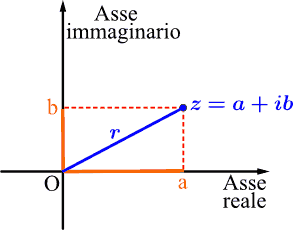
\includegraphics[width=0.3\textwidth]{Pictures/piano_gauss.png}
\end{figure}

\section{Alcune operazioni coi numeri complessi}
Avendo $z_1,z_2 \in \mathbb{C}$:

\subsection{Somma}
\begin{equation}
z_1+z_2 = x_1+x_2+i(y_1+y_2)
\end{equation}\\
In particolare:\\
$Re(z_1+z_2) = x_1+x_2$\\
$Im(z_1+z_2) = y_1+y_2$
\subsection{Prodotto}
\begin{equation}
z_1z_2 = x_1x_2-y_1y_2+i(x_1y_2+ x_2y_1)
\end{equation}\\
In particolare:\\
$Re(z_1z_2) = x_1x_2-y_1y_2$\\
$Im(z_1z_2) = x_1y_2 + x_2y_1$
\subsection{Modulo}
Avendo $z = x+iy \in \mathbb{C}$, si definisce il modulo di $z$ come:\\
\begin{equation}
|z| = \sqrt{x^2+y^2} \in \mathbb{R}
\end{equation}\\
Nel piano di Gauss, $|z|$ viene rappresentato come la distanza dal punto $z$ all'origine.

\section{Coniugato di z}
Con $z = x+iy \in \mathbb{C}$, si definisce il coniugato di $z$ come:
\begin{equation}
	\bar{z} = x-iy
\end{equation}

\section{Numeri complessi notevoli}
\subsubsection{Elemento neutro somma}
$0\ +\ i0$
\subsubsection{Elemento opposto somma}
$-x\ -\ iy$
\subsubsection{Elemento neutro prodotto}
$1\ +\ i0$
\subsubsection{Elemento reciproco prodotto}
\begin{Large}
$\frac{1}{z}=\frac{1}{x+iy}=\frac{x-iy}{x^2+y^2}$
\end{Large}


\subsubsection{Osservazioni}
Avendo $z_1,z_2 \in \mathbb{C}$, si può dimostrare:\\
\begin{equation}
\begin{gathered}
\overline{1+z_2} = \overline{z_1}+\overline{z_2}\\
\overline{z_1z_2} = \overline{z_1}\overline{z_2}\\
|\bar{z}| = |z|\\
z\bar{z}=|z|^2\\
\frac{1}{z} = \frac{\bar{z}}{|z|^2}
\end{gathered}
\end{equation}

\section{Rappresentazione trigonometrica}
Un numero complesso $z$ può inoltre essere definito come un vettore che ha per origine l'origine del piano di Gauss, come modulo il modulo di $z$ e come direzione un angolo $\theta$:\\
\begin{equation}
\begin{gathered}
z=r(cos(\theta)+isen(\theta)) =\\
r(cos(\theta+2k\pi)+isen(\theta+2k\pi)) \forall k \in \mathbb{Z}
\end{gathered}
\end{equation}

\begin{figure}[htbp]
	\centering
	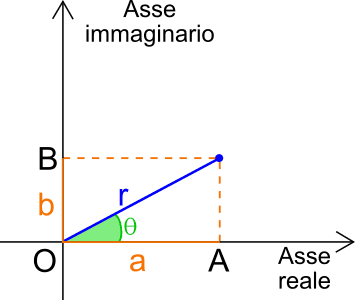
\includegraphics[width=0.3\textwidth]{Pictures/piano_gauss_trigonometria.png}
\end{figure}

In particolare:
\begin{enumerate}
	\item [i.] $r = |z| \geq 0$, in quanto il modulo di un numero complesso è per definizione positivo
	\item [ii.] $\theta$ è detto \textbf{argomento} di $z$
\end{enumerate}

\section{Operazioni con rappresentazione trigonometrica}
\subsection{Prodotto}
Con $z_1,z_2 \in \mathbb{C}$; definiamo $\theta_1 = argz_1,\ \theta_2=argz_2$:

\begin{equation}
z_1z_2=|z_1||z_2|(cos(\theta_1+\theta_2)+isen(\theta_1+\theta_2))
\end{equation}

\subsubsection{Dimostrazione}
\begin{equation*}
\begin{gathered}
z_1z_2=|z_1|(cos(\theta_1)+isen(\theta_1)) * |z_2|(cos(\theta_2)+isen(\theta_2)) =\\
|z_1||z_2|(cos(\theta_1)cos(\theta_2) + i^2sen(\theta_1)sen(\theta_2) + icos(\theta_1)sen(\theta_2) + isen(\theta_1)cos(\theta_2)) =\\
|z_1||z_2|((cos(\theta_1)cos(\theta_2)-sen(\theta_1)sen(\theta_2)) + i(cos(\theta_1)sen(\theta_2) + sen(\theta_1)cos(\theta_2))) =\\
z_1z_2=|z_1||z_2|(cos(\theta_1+\theta_2)+isen(\theta_1+\theta_2))
\end{gathered}
\end{equation*}

\subsection{Potenza (formula di De Moivre)}
Avendo $z \in \mathbb{C}$:\\
\begin{equation}
z^n = |z|^n(cos(n\theta)+isen(n\theta))
\end{equation}
\subsection{Radici n-esime}
$w,z \in \mathbb{C}$\; $n \in \mathbb{N}$\\
Se $n>1$, un numero $z$ è radice n-esima di $w \iff z^n=w$\\
Sia $w \in \mathbb{C}, n \in \mathbb{N}, n>1, w=|w|(cos(\theta)+isen(\theta)$:\\
\begin{enumerate}
\item[i.] Se $w=0$ la sola radice di $w$ è $z=0$
\item[ii.] Se $w\neq0$ allora $w$ ha \textbf{n} radici \textbf{distinte} che sono:\\
\begin{equation}
z_k=\sqrt[n]{|w|}(cos(\frac{\theta+2k\pi}{n})+isen(\frac{\theta+2k\pi}{n})),\ k \in \mathbb{N},\ 0\leq k<n
\end{equation}
\end{enumerate}
\subsubsection{Dimostrazione}
\begin{enumerate}
\item[i.]$w=0 \iff |z^n|=0 \iff |z|=0 \iff z=0$
\item[ii.]$z=|z|(cos(t)+isen(t))$; $z^n=w \iff \\
|z|^n(cos(nt)+isen(nt)) = |w|(cos(\theta+2k\pi)+isen(\theta +2k\pi) \iff
\begin{cases}
|z|^n = |w|\\
nt = \theta +2k\pi
\end{cases}$
\end{enumerate}
\subsection{Teorema fondamentale dell'algebra}
L'equazione polinomiale della forma: $a_nz^n + a_{n-1}z^{n-1}+...+a_1z+a_0$, $a_n \neq 0$, $a_i \in \mathbb{C}$ ha esattamente \textbf{n} radici in $\mathbb{C}$

\subsection{Notazione Esponenziale}
Per la formula di Eulero:\\
\begin{equation}
	e^{i\theta} = cos(\theta)+isen(\theta)
\end{equation}
Un numero complesso $z = |z|(cos(\theta)+isen(\theta))$ si può esprimere in notazione esponenziale come:\\
\begin{equation}
z = |z|e^{i\theta}
\end{equation}

\chapter{Il principio di induzione}
\section{Definizione di Pn}
$P_n$ è una proposizione (o affermazione) che dipende da n.

\section{Principio di induzione debole}
Sia $P_n$ una proposizione definita $\forall\ n>n_0$;  $n,n_0 \in \mathbb{N}$.
\begin{equation}
\begin{cases}
\textit{i. }P_{n_0}\ \text{è vero}\\
\textit{ii. }\forall\ n>n_0 \text{, supposta vera } P_n \text{ è vera anche } P_{n+1}
\end{cases} \iff P_n \text{ è vera}
\end{equation}
L'affermazione \textit{ii.} è chiamata \textbf{scatto induttivo}.

\section{Principio di induzione forte}
Sia $P_n$ una proposizione definita $\forall\ n>n_0$;  $n,n_0 \in \mathbb{N}$.
\begin{equation}
\begin{cases}
\textit{i. }P_{n_0}\ \text{è vero}\\
\textit{ii. }\forall\ n>n_0 \text{, supposte vere } P_{n_0},P_{n_0+1},...,P_n \text{ è vera anche } P_{n+1}
\end{cases} \iff P_n \text{ è vera}
\end{equation}

\section{Osservazione}
Varianti del problema possono porre come incognita anche $n_0$. In questo caso, conviene dimostrare inizialmente \textit{ii.} e poi cercare, fra i risultati ottenuti, il più piccolo numero $n_0 \in \mathbb{N}$ che soddisfi anche \textit{i.} .
\chapter{Funzioni}
\section{Definizione}
Dati due insiemi $\mathbb{X},\mathbb{Y}$ qualsiasi, una funzione di dominio $\mathbb{X}$ e valori in $\mathbb{Y}$ (=codominio) è una qualsiasi legge che ad ogni elemento di $\mathbb{X}$ associa un (e \textbf{uno solo}) elemento di $\mathbb{Y}$.
\begin{equation}
\begin{gathered}
f: \mathbb{X} \rightarrow \mathbb{Y}\\
x \rightarrow y=f(x)
\end{gathered}
\end{equation}

\section{Funzioni particolari}
\subsection{Funzione costante}
\begin{equation*}
\begin{gathered}
\bar{y} \in \mathbb{Y}, f: \mathbb{X} \rightarrow \mathbb{Y}\\
f(x)=\bar{y}\ \forall\ x \in \mathbb{X}
\end{gathered}
\end{equation*}
\subsection{Funzione identità}
\begin{equation*}
\begin{gathered}
I_x: \mathbb{X} \rightarrow \mathbb{X}\\
I_x(x)=x\ \forall\ x \in \mathbb{X}
\end{gathered}
\end{equation*}
\subsection{Funzione restrizione}
\begin{equation*}
\begin{gathered}
f: \mathbb{X} \rightarrow \mathbb{Y}; \mathbb{A} \subseteq \mathbb{Y}\\
f\restriction_\mathbb{A} =f(x)\ \forall\ x \in \mathbb{A}\\
f\restriction_\mathbb{A}: \mathbb{A} \rightarrow \mathbb{Y};\ x \rightarrow f(x)
\end{gathered}
\end{equation*}

\section{Insieme Immagine}
Sia $f: \mathbb{X} \rightarrow \mathbb{Y}$ e $\mathbb{A} \subseteq \mathbb{Y}$, diremo $\mathbb{A}$ tramite $f$ l'insieme $f(\mathbb{A}) = \{f(x) | x \in \mathbb{A}\}$.\\
Se $\mathbb{A} = \mathbb{X}$, $f(\mathbb{X})$ è semplicemente detta Immagine di $f$; $f(\mathbb{X}) = Imf$

\section{Iniettività, Suriettività e Biettività}
\subsection{Iniettività}
Una funzione $f: \mathbb{X} \rightarrow \mathbb{Y}$ si dice \textbf{iniettiva} se:
\begin{equation*}
\forall x_1,x_2 \in \mathbb{X}, x_1 \neq x_2, f(x_1) \neq f(x_2)
\end{equation*} 
Analogamente, il concetto di iniettività può essere definito come:
\begin{equation*}
f(x_1) = f(x_2) \iff x_1=x_2
\end{equation*}
Se la funzione \`e strettamente crescente o decrescente \`e iniettiva. $f:A \subset \mathbf{R}\rightarrow\mathbf{R}$ \`e iniettiva se ogni retta orizzontale interseca il suo 
grafico al pi\`u in un punto.
\subsection{Suriettività}
Una funzione $f: \mathbb{X} \rightarrow \mathbb{Y}$ si dice \textbf{suriettiva} se:
\begin{equation*}
\forall y \in \mathbb{Y}\ \exists\ x \in \mathbb{X}\ |\ f(x) = y
\end{equation*} 
Analogamente, il concetto di suriettività può essere definito come:
\begin{equation*}
Imf = \mathbb{Y}
\end{equation*}

\subsection{Biettività}
Una funzione $f: \mathbb{X} \rightarrow \mathbb{Y}$ si dice \textbf{biiettiva} se è sia iniettiva che suriettiva.
\begin{equation*}
f: \mathbb{X} \rightarrow \mathbb{Y}\ biettiva \iff \forall\ y \in \mathbb{Y}\ \exists !\ x \in \mathbb{X}\ |\ f(x)=y
\end{equation*}

\section{Grafico}
Sia $f: \mathbb{X} \rightarrow \mathbb{Y}$; si dice grafico di $f$ (indicato con $G(f)$ o $graph(f)$) il sottoinsieme di $\mathbb{X}\times\mathbb{Y}$ definito come:
\begin{equation*}
graph(f)=\{(x,f(x)), x \in \mathbb{X}\} \subseteq \mathbb{X}\times\mathbb{Y}
\end{equation*}
Spesso si usa impropriamente la parola \textit{funzione} per indicare il \textit{grafico di funzione}, ma è generalmente accettato a scopo di semplificazione del discorso.

\section{Altre funzioni particolari}
\subsection{Funzione parte intera}
\begin{equation}
\begin{gathered}
$[$\cdot$]$: \mathbb{R} \rightarrow \mathbb{R}\\
x \rightarrow [x] = max\{n \in \mathbb{Z} | n\leq x\}
\end{gathered}
\end{equation}

\subsection{Funzione di Heaviside}
\begin{equation}
\begin{gathered}
H: \mathbb{R} \rightarrow \mathbb{R}\\
x \rightarrow H(x) =
\begin{cases}
1 \text{  se } x \geq 0\\
0 \text{  se } x < 0
\end{cases}
\end{gathered}
\end{equation}

\subsection{Funzione segno}
\begin{equation}
\begin{gathered}
sgn: \mathbb{R} \rightarrow \mathbb{R}\\
x \rightarrow sgn(x) =
\begin{cases}
1 \text{ se } x > 0\\
0 \text{ se } x = 0\\
-1 \text{ se } x < 0
\end{cases}
\end{gathered}
\end{equation}

\subsection{Funzione mantissa}
\begin{equation}
\begin{gathered}
f: \mathbb{R} \rightarrow \mathbb{R}\\
x \rightarrow f(x) = x - $[$x$]$
\end{gathered}
\end{equation}

\subsection{Funzione parte positiva}
\begin{equation}
\begin{gathered}
f_+: \mathbb{X} \rightarrow \mathbb{R}\\
f_+(x)=\begin{cases}
f(x) \text{ se } x>0\\
0 \text{ se } x \leq 0\\
\end{cases}
\end{gathered}
\end{equation}

\subsection{Funzione parte negativa}
\begin{equation}
\begin{gathered}
f_-: \mathbb{X} \rightarrow \mathbb{R}\\
f_-(x)=\begin{cases}
-f(x) \text{  se } x<0\\
0 \text{  se } x \geq 0\\
\end{cases}
\end{gathered}
\end{equation}
\section{Operazioni tra funzioni}
\begin{itemize}
\item Somma di due funzioni: $(f\pm g)(x)\dot{=}f(x)\pm g(x) \forall x\in A$.
\item Prodotto di due funzioni: $(f\cdot g)(x)\dot{=}f(x)\cdot g(x) \forall x\in A$.
\item Rapporto di due funzioni: $\frac{f}{g}(x)\dot{=}\frac{f(x)}{g(x)}, \forall x\in A:g(x)\neq 0$.
\end{itemize}
\section{Trasformazioni di funzioni}
Una funzione pu\`o essere:
\begin{itemize}
\item Traslata verticalmente: $f(x)+a$, verso l'alto se a positivo, verso il basso se a negativo.
\item Traslata orizzontalmente: $f(x+a)$ verso sinistra se a positivo, verso destra se a negativo.
\item Dilatata verticalmente: $af(x)$: cambio di scala su asse Y, dilatazione se $a<1$, compressione se $0<a<1$, se $a<0$ il grafico viene riflesso rispetto all'asse X.
\item Dilatata orizzontalmente: $f(ax)$: cambio di scala su asse X, compressione se $a<1$, dilatazione se $0<a<1$, se $a<0$ il grafico viene riflesso rispetto all'asse Y.
\item Valore assoluto:
\begin{itemize}
\item $|f(x)|$ la parte negativa del grafico viene riflessa rispetto all'asse X.
\item $f(|x|)$ il grafico della parte negativa si trova riflesso rispetto all'asse Y nella parte negativa.
\end{itemize}
\end{itemize}
\section{Proprietà}
\subsection{Monotonia}
Sia $\mathbb{A} \subseteq \mathbb{X} \subseteq \mathbb{R}$ e $f: \mathbb{X} \rightarrow \mathbb{R}$ funzione detta (nell'insieme $\mathbb{A}$):
\begin{enumerate}
\item \textbf{crescente}: $\forall\ x_1,x_2 \in \mathbb{A}$, $x_1<x_2$; $f(x_1) \leq f(x_2)$
\item \textbf{strettamente crescente}: $\forall\ x_1,x_2 \in \mathbb{A}$, $x_1<x_2$; $f(x_1) < f(x_2)$
\item \textbf{decrescente}: $\forall\ x_1,x_2 \in \mathbb{A}$, $x_1<x_2$; $f(x_1) \geq f(x_2)$
\item \textbf{strettamente decrescente}: $\forall\ x_1,x_2 \in \mathbb{A}$, $x_1<x_2$; $f(x_1) > f(x_2)$
\item \textbf{monotona}: $f$ crescente oppure decrescente
\item \textbf{strettamente monotona}: $f$ strettamente crescente oppure strettamente decrescente
\end{enumerate}
\subsubsection{Osservazioni}
\begin{enumerate}
\item La somma di due funzioni crescenti è crescente;\\
La somma di due funzioni decrescenti è decrescente
\item Il prodotto di due funzioni crescenti non negative è crescente
\end{enumerate}
\subsection{Parità}
Sia $\mathbb{X}$ \textbf{simmetrico} rispetto l'origine (cioè: $\forall\ x \in \mathbb{X}$; $-x \in \mathbb{X}$); se $f: \mathbb{X} \rightarrow \mathbb{R}$ allora:
\begin{enumerate}
\item[i.] $f$ si dice \textbf{pari} in $\mathbb{X}$ se $f(x) = f(-x)\ \forall\ x \in \mathbb{X}$
\item[ii.] $f$ si dice \textbf{dispari} in $\mathbb{X}$ se $f(x) = -f(-x)\ \forall\ x \in \mathbb{X}$
\end{enumerate}
\subsection{Periodicità}
Sia $\mathbb{X} \subseteq \mathbb{R}$;   $f: \mathbb{X} \rightarrow \mathbb{R}$ si dice \textbf{periodica} di periodo $T>0$ se $T$ è il più piccolo numero reale tale che $x + T \in \mathbb{X}$, $f(x) = f(x + T)$\\
Ogni intervallo di lunghezza $T$ è detto intervallo di periodicità
\section{Estremi di funzione}
Sia $f: \mathbb{X} \rightarrow \mathbb{R}$
\subsection{Positività}
\begin{enumerate}
\item $f$ si dice \textbf{positiva} in $\mathbb{A} \subseteq \mathbb{R} \iff f(x)>0\ \forall\ x \in \mathbb{A}$
\item $f$ si dice \textbf{non negativa} in $\mathbb{A} \subseteq \mathbb{R} \iff f(x) \geq 0\ \forall\ x \in \mathbb{A}$
\item $f$ si dice \textbf{negativa} in $\mathbb{A} \subseteq \mathbb{R} \iff f(x)<0\ \forall\ x \in \mathbb{A}$
\item $f$ si dice \textbf{non positiva} in $\mathbb{A} \subseteq \mathbb{R} \iff f(x) \leq 0\ \forall\ x \in \mathbb{A}$
\end{enumerate}
\subsection{Limitazione, massimo assoluto, minimo assoluto, estremo superiore e inferiore e caratterizzazione}
Gli estremi assoluti di $f$ sono gli stessi dell'insieme $f(\mathbb{X}) = Immf$; per le definizioni fare quindi riferimento agli \hyperref[sec: estremiInsiemi]{\color{cyan}estremi di insiemi}.
\section{Successioni}
La funzione $f: \mathbb{N} \rightarrow \mathbb{R}$;  $n \rightarrow f(n) = a_n$ è chiamata successione e scritta anche come: $\{a_n\}_{n \in \mathbb{N}}$
\section{Composizione di funzioni}
Siano: $f: domf \rightarrow \mathbb{Y}$; $g: domg \rightarrow \mathbb{W}$ due funzioni e $\mathbb{A}=\{x \in domf\ |\ f(x) \in domg\}$. Si può allora definire:\\
\begin{equation}
\begin{gathered}
(g \circ f)(x) = g(f(x))\\
g \circ f: \mathbb{A} \in \mathbb{W}
\end{gathered}
\end{equation}
In particolare $\mathbb{A} \subseteq \mathbb{Y}$ ed è sempre definita $g \circ f \restriction _\mathbb{A}$
\subsubsection{Osservazione}
$f \circ g \neq g \circ f$
\subsection{Proprietà}
Sia $\mathbb{A} \subseteq dom(g \circ f)$.
\begin{enumerate}
\item[i.] $\begin{cases}
f \text{ crescente in } \mathbb{A}\\
g \text{ crescente in } f(\mathbb{A})
\end{cases} \implies g \circ f \text{ crescente}$
\item[ii.] $\begin{cases}
f \text{ crescente in } \mathbb{A}\\
g \text{ decrescente in } f(\mathbb{A})
\end{cases} \implies g \circ f \text{ decrescente}$
\item[iii.] $\begin{cases}
f \text{ decrescente in } \mathbb{A}\\
g \text{ crescente in } f(\mathbb{A})
\end{cases} \implies g \circ f \text{ decrescente}$
\item[iv.] $\begin{cases}
f \text{ decrescente in } \mathbb{A}\\
g \text{ decrescente in } f(\mathbb{A})
\end{cases} \implies g \circ f \text{ crescente}$
\end{enumerate} 
\section{Funzione inversa}
Sia $f: \mathbb{X} \rightarrow \mathbb{Y}$ una funzione biettiva. La \textbf{funzione inversa} di $f$ si definisce come:
\begin{equation}
\exists\ f^{-1}: \mathbb{Y} \rightarrow \mathbb{X};\ y \rightarrow x = f^{-1}(y)\ |\ f(x) = y
\end{equation}
Una funzione \`e invertibile se e solo se \`e iniettiva. La funzione inversa conserva la monotonia.
\subsection{Osservazioni}
\begin{enumerate}
\item $f^{-1}(f(x))=x\\
f(f^{-1}(y))=y$
\item Se $(y,x) \in graph(f^{-1}) \implies f^{-1}(y) = x \implies f(x)=y \implies (x,y) \in graph(f)$\\
(Il grafico di $f$ e di $f^{-1}$ sono simmetrici rispetto la bisettrice del primo e del terzo quadrante).
\end{enumerate}
\subsection{Funzioni goniometriche inverse}
Siano le funzioni goniometriche:
\begin{equation}
\begin{gathered}
sen: [-\frac{\pi}{2};\frac{\pi}{2}] \rightarrow [-1;1]\\
cos: [0;\pi] \rightarrow [-1;1]\\
tan: [-\frac{\pi}{2};\frac{\pi}{2}] \rightarrow \mathbb{R}
\end{gathered}
\end{equation}
Le funzioni inverse sono:
\begin{equation}
\begin{gathered}
arcsen: [-1;1] \rightarrow [-\frac{\pi}{2};\frac{\pi}{2}]\\
arccos: [-1;1] \rightarrow [0;\pi]\\
arctan: \mathbb{R} \rightarrow [-\frac{\pi}{2};\frac{\pi}{2}]
\end{gathered}
\end{equation}
\subsubsection{Osservazioni sulle funzioni goniometriche inverse}
\begin{itemize}
\item $\sin(\arcsin x)=x \forall x\in [-1,1]$.
\item $\arcsin(sinx)=x \forall x\in [-\frac{\pi}{2}, \frac{\pi}{2}], \forall x\in\mathbf{R}, \arcsin(\sin x)=x'$ dove x' \`e l'unico punto in $[-\frac{\pi}{2}, \frac{\pi}.
{2}]$ tale che $\sin x=\sin x'$.
\item $\cos(\arccos x)=x \forall x\in[-1,1].$
\item $\arccos(\cos x)=x \forall x\in\mathbf{R}, \arccos(\cos x)=x'$ dove x' \`e l'unico punto in $[-\frac{\pi}{2}, \frac{\pi}{2}]$ tale che $\cos x=\cos x'$.
\item $\tan(\arctan x)=x \forall x\in \mathbf{R}$.
\item$\arctan(\tan x)=x \forall x\in [-\frac{\pi}{2}, \frac{\pi}{2}], \forall x\in\mathbf{R}, \arctan(\tan x)=x'$ dove x' \`e l'unico punto in $[-\frac{\pi}{2}, \frac{\pi}.
{2}]$ tale che $\tan x=\tan x'$.
\end{itemize}
\subsection{Risoluzione di equazioni o disequazioni con metodo grafico}
Disegno la funzione sulla destra e quella sulla sinistra e successivamente ne considero la posizione reciproca. 
\chapter{Propriet\`a locali di una funzione}
\section{La vicinanza a un punto}
\subsection{La distanza}

La distanza in $\mathbb{R}$ \`e definita da $d(x, y)\dot{=}|x-y|,\forall x,y\in]\mathbb{R}, d(x, y)\ge 0, d(x,y)=0\Leftrightarrow x=y, d(x, y)=d(y, x), d(x, y)\le d(x,z)
+d(z,y)$, 
\section{L'intorno}
Fissati $x_0\in\mathbb{R}, \epsilon>0$, chiameremo intorno (sferico) di centro $x_0$ e raggio $\epsilon$, l'intervallo $]x_0-\epsilon; x_0+\epsilon[=\{x\in\mathbb{R}:d(x, x_0)<\epsilon\}$ $I_{x_0}$ \`e l'insieme degli intorni sferici di $x_0$ indicati come U, V, W.
\section{Estremi locali di una funzione}
$f:X\subset\mathbb{R}\rightarrow\mathbb{R},x_0\in X$, $x_0$ si dice punto di minimo locale di $f$ e $f(x_0)$ minimo locale se $\exists U\in I_{x_0}: f(x_0)\le f(x) \forall x\in U\cap X$, se manca l'uguale si dice punto di minimo locale stretto o forte per $f$, analogamente per il massimo.
\subsection{I numeri reali estesi}
Non \`e un insieme numerico $\bar{\mathbb{R}}\dot{=}\mathbb{R}\cup\{-\infty;+\infty\}$. 
\begin{itemize}
\item $-\infty<x<+\infty$
\item $x\pm\infty=\pm\infty$
\item $x\cdot \pm\infty=\pm\infty, x>0$ 
\item $x\cdot \pm\infty=\mp\infty, x<0$
\item Non \`e definita $+\infty-\infty$
\item Non \`e definita $0\cdot\pm\infty$
\item Non \`e definita $\frac{0}{0}$
\item Non \`e definita $\frac{\infty}{\infty}$
\end{itemize}
\subsection{Intorni sferici di $\pm\infty$}
Si dice intorno sferico di $+\infty$ qualunque semiretta $]M;+\infty[=\{ x\in\mathbb{R}:x>M\}$\\
Si dice intorno sferico di $-\infty$ qualunque semiretta $]M;-\infty[=\{x\in\mathbb{R}:x<M\}$\\
In $\bar{\mathbb{R}}$, l'insieme degli intorni $I_{x_0} $\`e dato da $I_{x_0}=\begin{cases}-\infty\\x_0\in\mathbb{R}\\+\infty\end{cases}$%Aggiungi rette
\subsection{Punto di accumulazione}
Sia $A\subset\mathbb{R}$; si dice che $x_0\in\bar{\mathbb{R}}$ \`e un punto di accumulazione per A se ogni intorno di $x_0$ contiene un punto di A diverso da $x_0$.\\
$\forall U\in I_{x_0}$ si ha $(U\backslash\{x_0\}\cap A\neq \emptyset$. In ogni intorno U di un punto di accumulazione cadono infiniti punti di A.\\
Unico punto di accumulazione in $\mathbb{N}$ \`e $+\infty$.\\
In ogni intorno U di un punto di accumulazione cadono infiniti punti di A.
\subsection{Punto isolato}
Un punto $x_0\in A$ che non \`e un punto di accumulazione per A si dice punto isolato, ossia $x_0\in A$ \`e isolato se $\exists U\in I_{x_0}:U\cup A=\{x_0\}$.\\ 
\chapter{Continuit\`a}
$f: X\subset\mathbb{R}\rightarrow\mathbb{R}, x_0\in X$ Se $x_0$ \`e un punto isolato di X f \`e continua nel punto isolato ed esso \`e un punto di accumulazione. Se $x_0$ \`e un punto di accumulazione per X f si dice continua in $x_0$ se $\exists \lim\limits_{x\rightarrow x_0} f(x)\wedge\lim\limits_{x\rightarrow x_0} f(x)=f(x_0)$
\section{Note}
f si dice continua in $x_0\in X \Leftrightarrow\forall\epsilon>0\exists\delta>0 :\forall x\in X:|x-x_0|<\delta \Rightarrow |f(x)-f(x_0)|<\epsilon$\\
Non ha senso parlare di continuit\`a per un punto che non appartiene al dominio della funzione.\\
Dalle proposizioni dei limiti se f e g sono continue in $x_0\in domf\cap domg$ anche somma, prodotto e rapporto sono continue in $x_0$.\\
Applicando il teorema dell'esistenza del limite sinistro e destro per una funzione monotona, si ottiene la continuit\`a nel loro dominio di tutte le funzioni elementari.\\
$\forall x_0\in\mathbb{R},\lim\limits_{x\rightarrow x_0} x^n=x_0^n$

\chapter{I limiti}
Esempi di definizione di limiti:
\begin{itemize}
\item $\lim\limits_{x\rightarrow x_0}f(x)=n\Leftrightarrow\forall \epsilon>0, \exists \delta<0: \forall x\in domf, 0<|x-x_0|<\epsilon\Rightarrow |f(x)-n|<\delta$\\
\item $\lim\limits_{x\rightarrow -\infty}f(x)=+\infty\Leftrightarrow\forall M>0, \exists k<0: \forall x\in domf, x<k\Rightarrow f(x)>M$\\
\item $\lim\limits_{x\rightarrow n}f(x)=+\infty\Leftrightarrow\forall M>0, \exists \delta<0: \forall x\in domf, 0<|x-n|<\delta\Rightarrow f(x)>M$\\
\end{itemize}
\section{Definizione unificata di limite}
$X\subset\mathbb{R}, f:X\rightarrow\mathbb{R}$, funzione, sia $x_0\bar{\mathbb{R}}$ punto di accumulazione per X. Allora $l\in\bar{\mathbb{R}}$ si dice limite per $f(x)$, per 
$x$ tendente a $x_0$, $\lim\limits_{x \rightarrow x_0}=l$ se $\forall V$, intorno di $l$, $\exists$ un intorno $U$ di $x_0$ tale che $\forall x\in (U\cap X)\backslash\{x_0\}$ si ha $f(x)\in V$. Non viene espresso il comportamento di $f$ in $x_0$ quando $x\rightarrow x_0$, $f$ pu\`o anche non essere definita in $x_0$
\subsection{Casi particolari}
$\lim\limits_{x\rightarrow -\infty} f(x)=+\infty$, intorni di $l=+\infty$ sono $]M,+\infty[$ con $M>0$.\\
Intorni di $x_0=-\infty$ sono $]-\infty,k[$ con $k<0$\\
Quindi $\forall M>0, \exists k<0:\forall x\in ]-\infty,k[\cap X$,\\
si ha $f(x)\in ]M,+\infty[$\\
$\Leftrightarrow \forall M>0, \exists k<0:\forall x\in X, x<k\Rightarrow f(x)>M$\\
$\lim_{x\rightarrow 2} f(x)=1$ intorni di 1 sono $]1-\epsilon;1+\epsilon[ (\epsilon>0)$, gli intorni di 2 sono $]2-\delta;2+\delta[(\delta>0)$. Quindi $\forall\epsilon>0, 
\exists \delta>0:\forall x\in X, |x-2|<\delta$ si ha $|f(x)-1|<\epsilon$.\\
\subsection{Note}
\begin{itemize}
\item U dipende da V
\item $x_0$ non deve appartenere al dominio della funzione, se appartiene non \`e detto che il limite sia uguale a $f(x_0)$
\item Se $l\in\mathbb{R}$ si dice che $f$ ammette limite finito per $x\rightarrow x_0$
\item $\lim\limits_{x\rightarrow x_0} f(x)=l\Leftrightarrow \lim\limits_{x\rightarrow x_0} (f(x)-l)=0$
\item $\lim\limits_{x\rightarrow x_0} f(x)=0 \Leftrightarrow\lim\limits_{x\rightarrow x_0} |f(x)|=0$
\item $l\neq 0$, pu\`o essere che $\nexists\lim\limits_{x\rightarrow x_0} f(x)$ ma $\exists \lim\limits_{x\rightarrow x_0} |f(x)|=l$
\end{itemize}
\section{Limitatezza}
Se una funzione ha limite finito, nell'intorno di $x_0$ la funzione \`e limitata.\\
$\lim\limits_{x\rightarrow x_0} f(x)=l\in\mathbb{R}$ allora $f$ \`e limitata in un intorno di $x_0$. 

\section{Teoremi generali}
\subsection{Unicit\`a del limite}
Se esiste il limite $\lim\limits_{x\rightarrow x_0} f(x)$ allora esso \`e unico.\\
\subsubsection{Dimostrazione}
Supponiamo per assurdo che esistano due limiti distinti:
\begin{center}
$\lim\limits_{x\rightarrow x_0} f(x)=l_1\neq l_2=\lim\limits_{x\rightarrow x_0} f(x)$
\end{center}
Esistono due intorni $V_1$ di $l_1$ e $V_2$ di $l_2$ tali che $V_1\cap V_2=\emptyset$. D'altra parte per definizione di limite, esistono due intorni $U_1$ di $x_0$ e $U_2$
di $x_0$  tali che 
\begin{center}
$f(x)\in V_1 \forall x\in (U_1\cap X)\backslash\{x_0\}$\\
$f(x)\in V_2 \forall x\in (U_2\cap X)\backslash\{x_0\}$
\end{center}
Allora per $x\in (U_1\cap U_2)\cap X\backslash\{x_0\}\Rightarrow f(x)\in V_1\cap V_2$ che contraddice il fatto che $V_1\cap V_2=\emptyset$.
\subsubsection{Dimostrazione}
Si fissi $\epsilon=1$. Allora $\exists U$ intorno di $x_0$: $\forall x\in U\cap domf\backslash\{x_0\}$ si ha $|f(x)-l|<\epsilon$ pertanto localmente \`e limitata in quanto
si trova ad una distanza finita $\epsilon$.
\subsection{Permanenza del segno}
Se una funzione ha limite positivo.
Sia $X\subset\mathbb{R}, f:X\rightarrow\mathbb{R}, x_0\in\bar{\mathbb{R}}$ punto di accumulazione, $l\in\bar{\mathbb{R}}$ allora esiste un intorno U tale che $f(x)>0$.
$\forall x\in U\cap X\backslash\{x_0\}$.
\subsubsection{Dimostrazione}
Supponiamo $l\in\mathbb{R},>0$. Nella definizione di limite consideriamo $\epsilon=\frac{l}{2}>0$ allora esiste U intorno di $x_0$ tale che $|f(x)-l|<\frac{l}{2}\forall x\in U\cap x\backslash\{x_0\}$. $0<\frac{l}{2}<f(x)<\frac{3l}{2}$.
Analogamente per infinito e l negativo.
\subsubsection{Note}
Non vale il viceversa: $f(x)=x^2>0 \forall$ intorno U di $x_0$ ma $\lim\limits_{x\rightarrow 0} f(x)=0$
\section{Esistenza del limite}
Il limite non esiste sempre, per esempio $\lim\limits_{n\rightarrow +\infty} (-1)^n=0$
\section{Punto di accumulzione sinistro e destro}
$x_0\in\mathbb{R}$ si dice punto di accumulazione sinistro (destro) per X se $x_0$ \`e un punto di accumulazione per $X\cap]-\infty;x_0[$ ($X\cap]-\infty;x_0[$)
\subsection{Intorno sinistro e destro}
Insiemi fatti da intervallo $]x_0-\epsilon;x_0[$, ($]x_0;x_0-\epsilon[$). Intorno sferico unione di intorno destro, sinistro e $x_0$.
\section{Teorema del confronto (dei due carabinieri)}
Siano $f,g,: X\rightarrow\mathbb{R}, x_0\in\bar{\mathbb{R}}$ punto di accumulazione per X.\\
$f(x)\le g(x)\le h(x), \forall x\in U\cap X\backslash\{x_0\}$ e se $\lim\limits_{x \rightarrow x_0} f(x)=\lim\limits_{x \rightarrow x_0} h(x)=l\in\bar{\mathbb{R}}$ allora $\lim\limits_{x \rightarrow x_0} g(x)=l$\\
Se $l=+\infty$ allora basta che $f(x)\le g(x)$\\
Se $l=-\infty$ allora basta che $f(x)\ge g(x)$\\
Il teorema del confronto si usa per studiare limiti di prodotti tra una funzione generale e una limitata ma il cui limite in tale punto non esiste.\\
$\lim\limits_{x\rightarrow 0} |x|^\alpha \sin\frac{1}{x}=0$\\
$\lim\limits_{x\rightarrow 0}\frac{1}{x}$ non esiste. Esiste con la x in modulo in quanto garantisce la costanza del segno nell'intorno.
\section{Forme indeterminate}
Una forma per cui non si pu\`o conoscere a priori il valore del limite.
\begin{itemize}
\item $+\infty-\infty$
\item $o\cdot\pm\infty$
\item $\frac{\infty}{\infty}$
\item $\frac{0}{0}$
\item $0^0$
\item $1^{\infty}$
\item $\infty^0$
\end{itemize}
\subsection{$\infty-\infty$}
\`E una forma indeterminata perch\`e consideriamo $x\rightarrow +\infty$
\\
\begin{tabular}{|c|c|c|}
\hline
$f(x)$ & $g(x)$ & $\lim\limits_{x\rightarrow +\infty} (f(x)+g(x))$\\
\hline
$x$ & $-\frac{x}{2}$ & $+\infty$\\
\hline
$x$ & $-2x$ & $-\infty$\\
\hline
$x$ & $-x+k$ & $k$\\
\hline
$x$ & $-x+\sin x$& $!\exists$\\ 
\hline
\end{tabular}
\subsection{$\frac{\infty}{\infty}$}
Se sono entrambi polinomi, se il grado del numeratore \`e maggiore fa infinito, se sono uguali fa il rapporto tra le incognite di grado massimo, se \`e minore fa zero.
Se aggiungo ai polinomi funzioni limitate non sono significative.
\subsection{$\frac{0}{0}$}
Pu\`o essere necessario scomporre per riuscire a semplificare la funzione.
\subsection{Trattare forme indeterminate}
Mettere in evidenza grado maggiore, razionalizzare, scomporre e altro.
\subsection{Funzione monotona e esistenza del limite sinistro e destro}
\subsubsection{Enunciato}
$f:X\subset\mathbb{R}\rightarrow\mathbb{R}$ funzione monotona, e f crescente in X, $x_0\in\mathbb{R}$ punto di accumulazione per X allora $\exists\lim\limits_{x\rightarrow x^-_0}
f(x)=sup f(x), x\in X\cap]-\infty, x_0[$\\
$\exists\lim\limits_{x\rightarrow x^+_0}f(x)=inf f(x) X\cap]x_0,+\infty[$.\\
Analogamente il caso di f decrescente.\\
\subsubsection{Dimostrazione}
Del limite sinistro. $l=\sup\limits_{X\cap]f-\infty, x_0[}$ Per definizione di l: $f(x)\le l \forall x\in X\cap]-\infty, x_0[$ e che $\forall \epsilon>0\exists x_\epsilon\in X
\cap]-\infty, x_0[: l-\epsilon\le f(x_\epsilon)\le f(x) \forall x\in X\cap]x_\epsilon, x_0[$ quindi $\forall\epsilon>0 \exists ]x_\epsilon, x_0[ l-\epsilon \le f(x)\le l<l+\epsilon\Leftrightarrow|f(x)-l|<\epsilon \forall x\in X\cap ]x_\epsilon, x_0[$ ho perci\`o dimostrato che il limite di l sia il sup. Se $l=+\infty$ allora f non \`e limitata
superiormente in $X\cap]-\infty;x_0[$, quindi $\forall M>0,\exists x_M\in X\cap]-\infty;x_0[:f(x_M)>M$, siccome f \`e crescente allora $M\le f(x_M)\le f(x)\forall x\in 
X\cap]x_M;x_0[$, ossia $\lim\limits_{x\rightarrow x_0^-}f(x)=+\infty$.\\
Nel caso in cui la funzione sia decrescente viene dimostrato analogamente.
\subsubsection{Corollari}
Sia $x_0\in\mathbb{R}$ punto di accumulazione per X e si supponga f monotona, allora $\exists\lim\limits_{x\rightarrow x_0^-}, \exists\lim\limits_{x\rightarrow x_0^=}$ ma non \`e detto che  $\exists\lim\limits_{x\rightarrow x_0}$, esiste solo se i due limiti sono uguali.
\subsubsection{Applicazioni}
$\lim\limits_{x\rightarrow +\infty} e^x= sup e^x=+\infty$\\
$\lim\limits_{x\rightarrow -\infty} e^x= inf e^x=+0$\\
$\lim\limits_{x\rightarrow +\infty} \arctan x= sup \arctan x=\frac{\pi}{2}$\\
Ho i limiti se conosco sup e inf, o viceversa.
\section{Limite di funzioni composte}
$f: X\subset\mathbb{R}\rightarrow\mathbb{R}, x_0$ punto di accumulazione per X.\\
$g: Y\subset\mathbb{R}\rightarrow\mathbb{R}, y_0$ punto di accumulazione per Y.\\
Se $\lim\limits_{x\rightarrow x_0} f(x)=y_0\;\lim\limits_{y\rightarrow y_0} g(y)=k$\\
$\lim\limits_{x\rightarrow x_0} g(f(x))=k$\\
$f(x)\neq y_0$ in un intorno U di $x_0$
\subsection{Osservazioni}
L'ipotesi che $f(x)\neq y_0$ in un intorno di di $x_0$ non \`e necessaria se $y_0\in Y\wedge g(y_0)=k$\\
Questo risultato si denota come cambiamento di variabili: $\lim\limits_{x\rightarrow x_0} g(f(x))=\lim\limits_{y\rightarrow y_0} g(y), f(x)=y\rightarrow y_0$\\
Dal teorema del limite per funzioni composte, segue che se $f$ \`e continua in $x_0\in X$ e se $g$ \`e continua in $y_0=f(x_0)\in Y$ allora $\lim\limits_{x\rightarrow x_0} g(f(x)=g(f(x_0))=(g\circ f)(x)$: la composta di funzioni continue \`e a sua volta continua.
\section{Esistenza del limite}
$\lim\limits_{x\rightarrow x_0}f(x)=l\Leftrightarrow\lim\limits_{x\rightarrow x_0^-}f(x)=l\wedge\lim\limits_{x\rightarrow x_0^+}f(x)=l$
\section{Algebra dei limiti}
Siano $f,g$ due funzioni e $x_0\in\bar{\mathbb{R}}$ un punto di accumulazione per entrambe. Supponiamo $\lim\limits_{x\rightarrow x_0^+}f(x)=l_f\in\mathbb{R}$ e $\lim
\limits_{x\xrightarrow{} x_0^+}g(x)=l_g\in\mathbb{R}$. Allora:
\begin{itemize}
\item $f(x)\pm g(x)\xrightarrow{x\rightarrow x_0} l_f\pm l_g$
\item $f(x) \cdot g(x)\xrightarrow{x\rightarrow x_0} l_f\cdot l_g$
\item $\frac{f(x)}{g(x)}\xrightarrow{x\rightarrow x_0}\frac{l_f}{l_g}$ Se $l_g\neq 0$
\end{itemize}
\section{Parziale estensione dell'algebra dei limiti a $\bar{\mathbb{R}}$}
Sia $x_0$ un punto di accumulazione per $domf\cap domg$, allora per $x\rightarrow x_0$ si ha:
\begin{itemize}
\item $f(x)\rightarrow+\infty$ e $g(x)$ limitata inferiormente nell'intorno di $x_0$, $\rightarrow f(x)+g(x)\xrightarrow[x\rightarrow x_0]{}+\infty$
\item $f(x)\rightarrow-\infty$ e $g(x)$ limitata superiormente nell'intorno di $x_0$, $\rightarrow f(x)+g(x)\xrightarrow[x\rightarrow x_0]{}-\infty$
\item $f(x)\rightarrow+\infty$ e $g(x)\rightarrow l_g\neq 0$, $\rightarrow f(x)\cdot g(x)\rightarrow 0$
\begin{itemize}
\item $\lim\limits_{x\rightarrow x_0}+\infty$ se $l_g>0$
\item $\lim\limits_{x\rightarrow x_0}-\infty$ se $l_g<0$
\end{itemize}
\item $f(x)\rightarrow 0$ e $g(x)$ limitata nell'intorno di $x_0$, $\rightarrow f(x)\cdot g(x)\xrightarrow[x\rightarrow x_0]{} 0$
\item $f(x)\rightarrow 0$
\begin{itemize}
\item $f(x)>0$ in un intorno di $x_0\rightarrow \frac{1}{f(x)}\xrightarrow[x\rightarrow x_0]{}+\infty$ 
\item $f(x)<0$ in un intorno di $x_0\rightarrow \frac{1}{f(x)}\xrightarrow[x\rightarrow x_0]{}-\infty$
\end{itemize}
\item $f(x)\rightarrow\pm\infty\rightarrow \frac{1}{f(x)}\xrightarrow[x\rightarrow x_0]{} 0 $
\end{itemize}
\subsection{Dimostrazione del teorema sull'algebra dei limiti}
Si ha $f(x)\xrightarrow{x\rightarrow x_0}l_f$ e $g(x)\xrightarrow{x\rightarrow x_0}l_g$ con $l_f,l_g\in\mathbb{R}$. Allora $f(x)\cdot g(x)\rightarrow l_f
\cdot l_g$ per $x\rightarrow x_0$.
Fissiamo $\epsilon>0$ arbitrario, dobbiamo verificare che esiste un intorno $U$ di $x_0$ tale che:
\begin{center}
$|f(x)\cdot g(x)-l_f\cdot l_g|<\epsilon, \forall x\in U\cap domf\cap domg\backslash\{x_0\}$
\end{center}
Per ipotesi: $|f(x)-l_f|<\epsilon\forall x\in U_f\cap domf\backslash\{x_0\}$ e $|g(x)-l_g|<\epsilon\forall x\in U_g\cap domg\backslash\{x_0\}$.\\
Si osservi che: $|f(x)g(x)-l_fl_g|=|f(x)g(x)-l_fg(x)+l_fg(x)l_fl_g|\le$\\
$\le |f(x)g(x)-l_fg(x)|+|l_fg(x)l_fl_g|\le$\\
$\le |g(x)||f(x)-l_f|+|l_f||g(x)-l_g|\le$\\
$\le M|f(x)-l_f|+|l_f||g(x)-l_g|$ in quanto $g$ ha limite finito, ovvero limitata in un intorno $\tilde{U}$ di $x_0$, ossia $\exists M>0:|g(x)<M\forall x\in\tilde{U}\cap 
domg\backslash\{x_0\}$\\
$\le (M+|l_f|)\epsilon$, abbiamo pertanto dimostrato che $|f(x)\cdot g(x)-l_f\cdot l_g|<\epsilon, \forall x\in U\cap domf\cap domg\backslash\{x_0\}$, dove $\epsilon$ \`e 
un numero arbitrario e $U=U_f\cap U_g\cap\tilde{U}$. Pertanto:
\begin{center}
$\lim\limits_{x\rightarrow x_0}f(x)\cdot g(x)=\lim\limits_{x\rightarrow x_0}f(x)\cdot \lim\limits_{x\rightarrow x_0}g(x)$
\end{center}
\section{Limiti notevoli per le funzioni trigonometriche}
\subsection{$\lim\limits_{x\rightarrow 0} \frac{\sin x}{x}=1$}
Dimostrazione: $x\in ]0,\frac{\pi}{2}[$, si disegni nella circonferenza goniometrica la tangente e il seno di x. L'area del triangolo formato tra origine e tangente \`e
 $\frac{\tan x}{2}$, l'area del triangolo formato da origine e il seno di x \`e $\frac{\sin x}{2}$, l'area del settore circolare individuato dall'asse delle x e il seno di x
 \`e $\frac{x}{2}$. Confrontando le aree $\forall x\in \mathbb{R}\backslash 0,\frac{\pi}{2}$: $\frac{\sin x}{2}<\frac{x}{2}<\frac{\tan x}{2}\Leftrightarrow$, dividendo per il seno 
 $1<\frac{x}{\sin x}<\frac{1}{\cos x}$, reciproci $\cos x<\frac{\sin x}{x}<1$, essendo il coseno e il rapporto pari si ottiene la stessa disuguaglianza $\forall x\in ]\frac{\pi}{2};]\frac{\pi}{2}\backslash\{0\}$, per il teorema del confronto ottengo $1<\frac{\sin x}{x}<1$, perci\`o $\sin x=1$
\subsection{$\lim\limits_{x\rightarrow 0} \frac{1-\cos x}{x^2}=\frac{1}{2}$}
$\frac{1-\cos x}{x^2}=\frac{1-\cos x}{x^2}\cdot\frac{1+\cos x}{1+\cos x}$\\
$=\frac{\sin^2 x}{x^2}\cdot\frac{1}{1+\cos x}$\\
$\lim\limits_{x\rightarrow 0}\frac{\sin^2 x}{x^2}=1$\\
$\lim\limits_{x\rightarrow 0}\frac{1}{1+\cos x}=\frac{1}{2}$\\
$\lim\limits_{x\rightarrow 0} \frac{1-\cos x}{x^2}=\frac{1}{2}$
\subsection{Corollari dei due limiti notevoli dimostrati sopra}
\begin{itemize}
\item $\lim\limits_{x\rightarrow 0} \frac{\tan x}{x}=1$
\item $\lim\limits_{x\rightarrow 0} \frac{\arcsin x}{x}=1$
\item $\lim\limits_{x\rightarrow 0} \frac{\arctan x}{x}=1$
\end{itemize}
\chapter{Gerarchia degli infiniti}
Per $x\rightarrow+\infty$: \\
\begin{center}
$|\log_b x|^\alpha<<x^\beta<<a^x$
\end{center}
\section{Osservazioni}
\begin{itemize}
\item $\lim\limits_{x\rightarrow+\infty}\frac{x^\beta}{a^x}=0$
\item $\lim\limits_{x\rightarrow+\infty} \frac{|\log_b x|^\alpha}{x^\beta}=0$
\item $\lim\limits_{x\rightarrow-\infty} a^x|x|^\beta=0$
\item $\lim\limits_{x\rightarrow 0^+} x^\beta|\log_b x|^\alpha=0$
\end{itemize}
Gli ultimi due si dimostrano con cambio di variabile in modo che il limite tenda a $+\infty$.
\section{Dimostrazione}
Si provi che $\lim\limits_{x\rightarrow+\infty}\frac{x}{4^x}=0$.\\
Dal grafico si nota che $2^x\ge x\forall x\ge 0$\\
$2^x\ge 2^{[x]}=(1+1)^{[x]}\ge 1+[x]$(per la disuguaglianza di Bernoulli).\\
$1+[x]\ge 1+x-1$\\
Ovvero $2^x\ge x$\\
$0<\frac{x}{4^x}=\frac{x}{2^x2^x\le \frac{1}{2^x}}$\\
Essendo che per $x\rightarrow +\infty$ o e $\frac{1}{2^x}$ tendono a 0,\\
$\lim\limits_{x\rightarrow+\infty}\frac{x}{4^x}=0$.\\
Per dimostrare che $\lim\limits_{x\rightarrow+\infty}\frac{x^\beta}{a^x}=0$\\
Si osservi che $a^x=4^{\log_4 a^x}$.\\
Perci\`o: $\frac{x^\beta}{a^x}=(\frac{x}{4^{x\frac{\log_4 a}{\beta}}})^\beta$\\
Ponendo $y=x4^{\frac{\log_4 a}{\beta}}$\\
$(\frac{y\beta}{\log_4 a}\frac{1}{4^y})^\beta$\\
$(\frac{\beta}{\log_4 a}\frac{y}{4^y})^\beta$\\
Si osserva che la prima frazione \`e una costante, mentre la seconda \`e il limite dimostrato all'inizio della sezione, pertanto:\\
$\lim\limits_{x\rightarrow+\infty}\frac{x^\beta}{a^x}=0$.\\
Partendo da questa dimostrazione si dimostra che $\lim\limits_{x\rightarrow+\infty} \frac{|\log_b x|^\alpha}{x^\beta}=0$, sostituendo $x$ con $y=\log_b x$
\section{Altre forme indeterminate}
$\lim\limits_{x\rightarrow x_0} f(x)^{g(x)}, f(x)>0$, $f(x)^{g(X)}=e^{\log f(x)\cdot g(x)}$
\begin{itemize}
\item $0^0$
\item $\infty^0$
\item $1^\infty$
\end{itemize}
Per calcolare i primi due gerarchie degli infiniti, mentre il terzo ci saranno dei limiti notevoli:
\begin{itemize}
\item $\lim\limits_{x\rightarrow 0}\frac{e^x-1}{x}=1$
\item $\lim\limits_{x\rightarrow 0}\frac{\log (x+1)}{x}=1$
\end{itemize}
\subsection{Limiti di successioni-esercizi}
$\lim\limits_{n\rightarrow +\infty}\sqrt[n]{n}=1$\\
$\lim\limits_{n\rightarrow +\infty}\sqrt[n]{n\log n}=1$ Osservazione: $1\le\log n\le n\Leftrightarrow n\le n\log n\le n^2\Leftrightarrow \sqrt[n]{n}\le\sqrt[n]{n\log n} \le \sqrt[n]{n^2}$\\
$\lim\limits_{n\rightarrow +\infty}\frac{n^\alpha}{a^n}=0\forall\alpha\in\mathbb{R}$\\
$\lim\limits_{n\rightarrow +\infty}\frac{{|\log_b n|}^{\alpha}}{n^{\beta}}=0\forall b>0,\neq 1,\forall\beta>0$\\
$\lim\limits_{n\rightarrow +\infty}\frac{a^n}{n!}=0\forall a>0$
\subsection{Gerarchia di infiniti per le successioni}
$\log_b n <<n^\alpha<<a^n<<n!<<n^n$
\subsubsection{Formula di Stirling}
$n!\sim (\frac{n}{e})^n\sqrt{2\pi n}$
\subsubsection{Il numero di Nepero $e$}
la successione $a_n=(1+\frac{1}{n})^n$ \`e strettamente crescente e limitata.\\
Per dimostrare che sia crescente considero $\frac{a_n}{a_{n-1}}<1$\\
$\frac{(1+\frac{1}{n})^n}{(1+\frac{1}{n-1})^{n-1}}=$\\
$(\frac{n+1}{n})^n(\frac{n-1}{n})^{n-1}=\frac{(\frac{n+1}{n})^n(\frac{n+1}{n})^n}{\frac{n-1}{n}}=$\\
$=\frac{(\frac{n^2-1}{n^2})^n}{(1-\frac{1}{n})}=$\\
$=\frac{(1-\frac{1}{n^2})^n}{(1-\frac{1}{n})}$\\
Che per la disuguaglianza di Bernoulli con $c=\frac{1}{n^2}$\\
$>\frac{1-\frac{1}{n}}{1-\frac{1}{n}}=1$.\\
Ossia $a_n>a_{n-1}$, la funzione \`e crescente.\\
Per dimostrare che \`e limitata considero:\\
$2\le (1+\frac{1}{n})^n\le (1+\frac{1}{n})^{n+1}\le 4$\\
Si dimostra, sempre utilizzando Bernoulli che il terzo termine \`e decrescente, pertanto:\\
$2\le (1+\frac{1}{n})^n\le 4$\\
Dal teorema dell'esistenza del limite per funzioni monotone determiniamo che esiste il limite finito:\\
$e\dot{=}\lim\limits_{x\rightarrow +\infty} (1+\frac{1}{n})^n$ che \`e l'estremo superiore.
\subsubsection{Corollario}
\begin{itemize}
\item $\lim\limits_{x\rightarrow+\infty} (1+\frac{1}{x})^x=e$
\item $\lim\limits_{x\rightarrow-\infty} (1+\frac{1}{x})^x=e$
\item $\lim\limits_{f(x)\rightarrow 0} (1+f(x))^\frac{1}{f(x)}=e$
\end{itemize}
Per dimostrare basta osservare che $\forall x\in\mathbb{R}, [x]\le x\le [x]+1:(1+\frac{1}{[x]+1})^{[x]}\le(1+\frac{1}{x})^x\le(1+\frac{1}{[x]})^{[x]+1}$. Gli estremi tendono
a $e$, pertanto per il teorema del confronto anche il secondo. Il secondo e terzo corollario si dimostrano in maniera analoga sostituendo la variabile rispettivamente con
$y=-x$ e con $y=\frac{1}{x}$.
\subsubsection{Corollario 2}
\begin{itemize}
\item $\lim\limits_{x\rightarrow 0} \frac{\log (1+x)}{x}=1$
\item $\lim\limits_{x\rightarrow 0} \frac{e^x-1}{x}=1$
\end{itemize}
Per dimostrarli bisogna considerare la continuit\`a del logaritmo e che $\frac{\log (1+x)}{x})=\log (1+x)^{\frac{1}{x}}$
\subsubsection{Corollario 3}
\begin{itemize}
\item $\lim\limits_{x\rightarrow 0} \frac{a^x-1}{x})=\log a$
\item $\lim\limits_{x\rightarrow\pm\infty} (1+\frac{\alpha}{x})^x=e^\alpha$
\item $\lim\limits_{x\rightarrow 0} (1+\alpha x)^\frac{1}{x}=e^\alpha$
\end{itemize}
Si utilizzano gli altri limiti notevoli considerando la x come una funzione continua.
\chapter{Infinito}
Una funzione $f:X\rightarrow \mathbb{R}, x_0\in\bar{\mathbb{R}}$ punto di accumulazione. Se $\lim\limits_{x\rightarrow x_0}f(x)=\pm\infty$ si dice divergente positivamente o 
negativamente.
\section{Confronto di infiniti}
Dette $f,g,x_0\in\bar{\mathbb{R}}$ punto di accumulazione. Se f e g sono entrambe infinite e $\lim\limits_{x\rightarrow x_0}\frac{f(x)}{g(x)}=0$ f \`e un infinito di ordine 
inferiore rispetto a g. Se invece $\lim\limits_{x\rightarrow x_0}\frac{f(x)}{g(x)}=l, l\in\bar{\mathbb{R}}\backslash 0$, f e g sono infiniti dello stesso ordine, in 
particolare, se $l=1$ allora si usa la notazione $f\sim g$ e si dice che f \`e asintotico a g per x che tende a $x_0$. Se invece $\lim\limits_{x\rightarrow x_0}\frac{f(x)}
{g(x)}=\infty$ allora si dice che f \`e un infinito di un ordine superiore rispetto a g. Se il limite non esiste allora si dicono non confrontabili.   
\section{Infinitesimi}
$f(x)\rightarrow l $ per $x\rightarrow x_0\Leftrightarrow f(x)-l=o(1)$. Quando indico con o(1) l'infinitesimo, ovvero un valore pi\`u piccolo vicino a 0.
\subsection{Regole di calcolo per o(1)}
\begin{itemize}
\item $ko(1)=o(1),\forall k\in\mathbb{R}$
\item $o(1)o(1)=o(1)$
\item $o(1)+o(1)=o(1)$
\item $o(1)-o(1)=o(1)$
\end{itemize}
\section{Confronto di infinitesimi}
Dette $f,g,x_0\in\bar{\mathbb{R}}$ punto di accumulazione. Se f e g sono entrambe infinitesime e $g(x)\neq $ e $\lim\limits_{x\rightarrow x_0}\frac{f(x)}{g(x)}=0$ si dice 
che f \`e  un infinitesimo di ordine superiore g, se vale $\infty$ \`e di ordine inferiore.  $\lim\limits_{x\rightarrow x_0}\frac{f(x)}{g(x)}=l$ sono dello stesso ordine e 
se $l=1$ f e g sono asintotiche. Se non esistono i limiti i due non sono confrontabili.
\section{Definizione}
Date due funzioni $f$ e $g$, $x_0\in\mathbb{\bar{R}}$ punto di accumulazione per $domf\cap domg$ e $g(x)\neq 0$, $f(x)=o(g(x))$ per $x\rightarrow x_0$ se $\lim\limits_{x
\rightarrow x_0}\frac{f(x)}{g(x)}=0$.
\subsection{Osservazioni}
\begin{itemize}
\item Se $f$ e $g$ sono entrambe infinite per $x\rightarrow x_0$ allora $f(x)=o(g(x))$ $f$ \`e un infinito di ordine inferiore rispetto a $g$.
\item Se $f$ e $g$ sono entrambe infinitesime per $x\rightarrow x_0$ allora $f(x)=o(g(x))$ $f$ \`e un infinitesimo di ordine superiore rispetto a $g$.
\end{itemize}
\section{regole di calcolo degli $o(x^\alpha)$}
Siano $\alpha,\beta>0\in\mathbb{R}$.
\begin{itemize}
\item $ko(x^\alpha)=o(x^\alpha)$ ($\frac{kf(x)}{x^\alpha}=k\frac{f(x)}{x^\alpha}$)
\item $x^\beta o(x^\alpha)=o(x^{\alpha+\beta})$ ($f(x)=o(x^\alpha)\,\frac{x^\beta f(x)}{x^{\alpha+\beta}}\:x^\beta f(x)=o(x^{\alpha+\beta})$)
\item $o(x^\alpha)\cdot o(x^\beta)=o(x^{\alpha+\beta})$ ($f(x)=o(x^\alpha), g(x)=o(x^\beta)\:\frac{f(x)g(x)}{x^{\alpha+\beta}}$)
\item $o(o(x^\alpha))=o(x^\alpha)$
\item $o(x^\alpha)\pm o(x^\beta)=o(x^\alpha)$ se $\alpha<\beta$ ($\frac{f(x)+g(x)}{x^\beta}=\frac{f(x)}{x^\alpha}+\frac{g(x)}{x^\alpha}\frac{x^\beta}{x^\beta}$)
\item $o(x^\alpha)\pm o(x^\beta)=o(x^\beta)$ se $\beta<\alpha$
\item $o(x^\alpha\pm x^{\alpha+\beta})=o(x^\alpha)$
\end{itemize}
\section{Linguaggio degli "o-piccoli" nel calcolo dei limiti}
Per $x\rightarrow 0 $, $\sin x= x-\frac{x^3}{3!}+o(x^3)$.
\section{Ordine di infinitesimo e di infinito}
$f,g$ funzioni infinitesime per $x\rightarrow x_0$, $g(x)\neq 0$ in un intorno di $x_0$ se $\exists\alpha>0, l\in\mathbb{R}\backslash\{0\}:\lim\limits_{x\rightarrow x_0}
\frac{f(x)}{|g(x)|^\alpha}=l$ allora $f$ \`e di ordine $\alpha$ rispetto all'infinitesimo campione $g(x)$ , per $x\rightarrow x_0$.\\ 
\begin{tabular}{|c c|c c|}
\hline
\multicolumn{2}{|c|}{$f$ infinitesimo} & \multicolumn{2}{c|}{$f$ infinito}\\
\hline
$x_0=0$&$g(x)=x$& $x_0=0$ & $g(x)=\frac{1}{x}$\\
$x_0\neq 0$&$g(x)=x-x_0$& $x_0\neq 0$ & $g(x)=\frac{1}{x-x_0}$\\
$x_0=\pm\infty$&$g(x)=\frac{1}{x}$& $x_0=\pm\infty$ & $g(x)=x$\\
\hline
\end{tabular}
\subsection{Definizione}
Se $f$ \`e un infinitesimo di ordine $d$ rispetto all'infinitesimo campione $x$ per $x\rightarrow 0^+$ si scrive che
\begin{equation}
f(x)=lx^\alpha+o(x^\alpha)\;x\rightarrow 0^+
\end{equation}
Dove $\lim\limits_{x\rightarrow 0^+}\frac{f(x)}{x^\alpha}=l\in\mathbb{R}\backslash\{0\}$, e $\alpha$ si dice ordine di infinitesimo e $lx^\alpha$ si dice parte principale
di infinitesimo. Pi\`u in generale:
\begin{equation}
f(x)=l(x-x_0)^\alpha+o((x-x_0)^\alpha)\;x\rightarrow x_0^+\in\mathbb{R}
\end{equation} 

\chapter{Asintoti}
Studio pi\`u dettagliato della crescita di funzioni all'infinito del dominio, ai punti di accumulazione non appartenenti al dominio o ai punti di discontinuit\`a.
\section{Asintoto orizzontale}
Sia $f$ una funzione definita in un intorno di $\pm\infty$, se $\lim\limits_{x\rightarrow\pm\infty}f(x)=b\in\mathbb{R}$ allora la retta $y=b$ si dice asintoto orizzontale per $f
$ per $x\rightarrow\pm\infty$
\section{Asintoto obliquo}
Sia $f$ una funzione definita in un intorno di $\pm\infty$, se esistono $a\neq 0$ e $b\in\mathbb{R}$ tali che$\lim\limits_{x\rightarrow\pm\infty}[f(x)-(ax+b)]=0$ allora la 
retta $y=ax+b$ si dice asintoto obliquo per $f$, per $x\rightarrow\pm\infty$.
\begin{equation}
\lim\limits_{x\rightarrow\pm\infty}[f(x)-(ax+b)]=0\Leftrightarrow
\begin{cases}
\lim\limits_{x\rightarrow\pm\infty}\frac{f(x)}{x}=a\\
\lim\limits_{x\rightarrow\pm\infty}(f(x)-ax)=b
\end{cases}
\end{equation}
\section{Asintoto verticale}
Sia $f:\mathbb{X}\subset\mathbb{R}\rightarrow\mathbb{R}$ una funzione e $x_0$ punto di accumulazione per $domf$. Se $\lim\limits_{x\rightarrow x_0^\pm}f(x)=\pm\infty$ allora
la retta verticale $x=x_0$ si dice asintoto verticale per $f$.
\subsection{Asintoto verticale da destra}
\begin{equation}
\lim\limits_{x\rightarrow x_0^+}f(x)=\pm\infty
\end{equation}
\subsection{Asintoto verticale da sinistra}
\begin{equation}
\lim\limits_{x\rightarrow x_0^-}f(x)=\pm\infty
\end{equation}
\chapter{Teorema ponte}
Lega il limite di funzioni con il limite di successioni. Sia $f:\mathbb{X}\rightarrow\mathbb{R}, x_0$ punto di accumulazione per $\mathbb{X}$ allora $\lim\limits_{x
\rightarrow x_0}f(x)=l\in\mathbb{\bar{R}}\Leftrightarrow\forall$ successione $\{x_n\}_n$ a valori in $\mathbb{X}\backslash\{x_0\}$, $x_n\rightarrow x_0$, 
\begin{equation}
\lim\limits_{x\rightarrow x_0}f(x_n)=l
\end{equation}
\section{Dimostrare che un limite non esiste}
\subsubsection{Esempio}
$\lim\limits_{x\rightarrow\infty}\sin x \:\nexists$. Basta prendere:\\
$x_n=\frac{\pi}{2}+2n\pi\xrightarrow[n\rightarrow+\infty]{}=+\infty$,\\
$\tilde{x_n}=\frac{3\pi}{2}+2n\pi\xrightarrow[n\rightarrow+\infty]{}=+\infty$. Da questi ottengo:\\ 
$f(x_n)=\sin x_n=1\xrightarrow[n\rightarrow \infty]{}1$\\
$f(\tilde{x_n})=\sin \tilde{x_n}=-1\xrightarrow[n\rightarrow \infty]{}-1$\\
Perci\`o essendo $f(x_n)\neq f(\tilde{x_n})$ il limite non esiste.
\section{Trovare il valore del limite quando esiste}
\subsection{Esempio}
$\lim\limits_{x\rightarrow+\infty}\log x$, il logaritmo \`e crescente, pertanto il limite esiste. Prendo come $x_n=e^n\xrightarrow[n\rightarrow+\infty]{}+\infty$,\\
$\log x_n=\log e^n=n\log e=n\Rightarrow\lim\limits_{n\rightarrow+\infty}\log x_n=\lim\limits_{n\rightarrow+\infty} n=+\infty$, pertanto per il teorema ponte segue che 
$\lim\limits_{x\rightarrow+\infty}\log x=+\infty$

\chapter{Continuit\`a e teoremi fondamentali}
\section{Punti di discontinuit\`a}
\begin{itemize}
\item $\exists\lim\limits_{x\rightarrow x_0}f(x)\neq f(x_0)$
\item $\exists\lim\limits_{x\rightarrow x_0^-}f(x)=f(x_0)\neq\lim\limits_{x\rightarrow x_0^+}f(x)$
\item $\exists\lim\limits_{x\rightarrow x_0^-}f(x)\neq f(x_0)\neq\lim\limits_{x\rightarrow x_0^+}f(x)$
\item $\exists\lim\limits_{x\rightarrow x_0^+}f(x)=f(x_0)\neq\lim\limits_{x\rightarrow x_0^-}f(x)=\infty$
\item $\exists\lim\limits_{x\rightarrow x_0^-}f(x)=f(x_0),\nexists\lim\limits_{x\rightarrow x_0^+}f(x)$
\end{itemize}
\section{Teorema della permanenza del segno}
Si deduce dal teorema della permanenza del segno per il limite: sia $f:domf\subset\mathbb{R}\rightarrow\mathbb{R}$ continua in $x_0\in domf$ e $f(x_0)>0$, analogo se 
negativo. Allora $\exists$ un intorno $U$ di $x_0$: $f(x)>0\forall x\in U\cap domf$.
\section{Teorema di esistenza degli zeri}
Un punto $x_0\in domf$ si dice uno zero di $f$ se $f(x_0)=0$. Il seguente teorema d\`a condizioni sufficienti affinch\`e $f$ abbia uno zero. La dimostrazione si basa sul 
metodo di bisezione.\\
Sia $f:[a;b]\rightarrow\mathbb{R}$, $f$ continua e $f(a)f(b)<0$, allora $\exists x_0\in]a,b[:f(x_0)=0$.\\
Se $f$ \`e strettamente monotona, allora $x_0$ \`e unico.
\subsection{Osservazioni}
\begin{itemize}
\item Togliendo una delle ipotesi l'esistenza non \`e garantita: se non \`e continua e con segni opposti lo zero potrebbe non esistere (funzione a tratti).
\item Pu\`o esistere uno zero per $f$ anche se manca una delle ipotesi, ma non \`e certo: $x^2$ tra $[-1;1]$.
\end{itemize}
\subsection{Dimostrazione}
Non \`e restrittivo considerare $f(a)<0$ e $f(b)>0$. Utilizzo il metodo di bisezione: ponendo $a_0=a$ e $b_0=b$, considero il loro punto medio $c_0=\frac{a_0+b_0}{2}$.
\begin{itemize}
\item Se $f(c_0)=0$ ho trovato lo zero della funzione.
\item Se $f(c_0)<0$ si pone $a_1=c_0$ e $b_1=b_0$.
\item Se $f(c_0)>0$ si pone $a_1=a_0$ e $b_1=c_0$.
\end{itemize}
In ogni caso $f(a_1)<0$ e $f(b_1)>0$ e $b_1-a_1=\frac{b-a}{2}$.\\
Ripetendo il ragionamento si consideri il punto medio di $[a_1;b_1]$, cio\`e $c_1=\frac{b_1+a_1}{2}$.
\begin{itemize}
\item Se $f(c_1)=0$ ho trovato lo zero della funzione.
\item Se $f(c_1)<0$ si pone $a_2=c_0$ e $b_2=b_1$.
\item Se $f(c_1)>0$ si pone $a_2=a_1$ e $b_2=c_1$.
\end{itemize}
In ogni caso $f(a_2)<0$ e $f(b_2)>0$ e $b_2-a_2=\frac{b-a}{2^2}$.\\
In questo modo $\forall n\ge 0$:\\
\begin{equation}
a\le a_1\le a_2\le\cdots\le a_n<b_n\le\cdots\le b_2\le b_1\le b
\end{equation}
Si trovano perci\`o due successioni$\{a_n\}$ crescente e $\{b_n\}$ decrescente.$\Rightarrow$
\begin{center}
$a_n\xrightarrow[n\rightarrow +\infty]{}x_0$\\
$b_n\xrightarrow[n\rightarrow +\infty]{}x_1$
\end{center}
Poich\`e $b_n-a_n=\frac{b-a}{2^n}$ e siccome per $n\rightarrow+\infty,\frac{b-a}{2^n}=0$ e $b_n\xrightarrow[n\rightarrow+\infty]{} x_1$ e 
$a_n\xrightarrow[n\rightarrow+\infty]{}x_0$, allora $x_1-x_0=0\Rightarrow x_1=x_0$\\
Basta provare che $f(x_0)=0$: $f(a_n)<0$ per il teorema ponte $f(a_n)\xrightarrow[n\rightarrow+\infty]{} f(x_0)\le 0$,\\
$f(b_n)>0$, per il teorema ponte $f(b_n)\xrightarrow[n\rightarrow+\infty]{}f(x_1)\ge 0$.
Ovvero $0\le f(x_0)\le 0$, da cui $f(x_0)=0$.
\subsection{Corollario 1}
Siano $f, g:[a;b]\rightarrow\mathbb{R}$ due funzioni continue, $f,g$, se $f(a)>g(x)$ e $f(b)<g(b)$ o viceversa, allora $\exists x_0\in]a;b[:f(x_0)=g(x_0)$.
\subsubsection{Dimostrazione}
Si ponga $h(x)\dot{=}f(x)-g(x)$ su $[a;b]$
\begin{itemize}
\item $h$ \`e continua su [a;b]
\item $h(a)=f(a)-g(a)>0$.
\item $h(b)=f(b)-g(b)<0$.
\end{itemize}
Il teorema di esistenza degli zeri ci garantisce che $\exists x_0\in ]a;b[:h(x_0)=0$, ossia $f(x_0)-g(x_0)=0\Rightarrow f(x_0)=g(x_0)$
\subsection{Corollario 2, teorema dei valori intermedi}
Sia $I$ intervallo $\subset\mathbb{R}$. Sia $f:I\rightarrow\mathbb{R}$ continua. Allora esistono $\inf\limits_I f$, $\sup\limits_I f$ e la funzione assume tutti i valori 
tra il limite inferiore e il limite superiore.
\subsubsection{Dimostrazione}
Se $\inf\limits_I f=\sup\limits_I f$ la funzione \`e costante e la tesi \`e ovvia. Altrimenti sia $\inf\limits_I f<y<\sup\limits_I f$ e proviamo che esiste $x\in I:y=f(x)$.\\
Per la definizione di $\inf\limits_I f,\exists a\in I:f(a)<y$ e per definizione di $\sup\limits_I f, \exists b\in I:y<f(b)$.\\
Perci\`o $f(a)<y<f(b)$. Si definisca la funzione $g(x)=y\;\forall x\in I$. Pertanto $f(a)<g(a)<y<g(b)<f(b)$.\\
Per il corollario precedente $\exists x\in I:f(x)=g(x)=y$.
\subsection{Corollario 3}
Considero $I$ intervallo $\subset\mathbb{R},f:I\rightarrow\mathbb{R}$ continua, allora $f(I)$ \`e un intervallo tra $\inf\limits_I f$ e $\sup\limits_I f$.
\section{Legame tra monotonia, iniettivit\`a, continuit\`a di $f$ su un intervallo}
\begin{itemize}
\item $f:domf\subset\mathbb{R}\rightarrow\mathbb{R}$, se la funzione \`e strettamente monotona la funzione \`e iniettiva.
\item L'iniettivit\`a non implica necessariamente la stretta monotonia.
\item La funzione inversa $f^{-1}:f(A)\rightarrow A$ di una funzione iniettiva, suriettiva e continua $f:A\subset\mathbb{R}\rightarrow f(A)$ risulta continua se il suo 
insieme immagine \`e un intervallo.
\end{itemize}
\subsection{Iniettivit\`a implica la monotonia}
L'iniettivit\`a di una funzione ne implica la monotonia se $f$ \`e continua: $f:I\subset\mathbb{R}\rightarrow\mathbb{R}$, con $I$ intervallo e $f$ continua e iniettiva, \\
allora $f$ \`e strettamente monotona in $I$.
\subsubsection{Dimostrazione}
Si procede per assurdo: si supponga che la funzione non sia strettamente monotona, pertanto $\exists x<y<z\in I:f(y)>f(x)>f(z)$. Per il teorema dei valori intermedi applicato
su $[y;z]\Rightarrow\exists\bar{x}\in[y;z]:f(x)=f(\bar{x})$, che contraddice il fatto che $f$ sia iniettiva. Ho raggiunto un assurdo, pertanto il teorema \`e dimostrato.
\section{Teorema di Weierstrass}
Esiste sempre $\inf\limits_A f$ e $\sup\limits_A f$, ma non esistono sempre il minimo e il massimo. Questo teorema stabilisce le condizioni sufficienti per l'esistenza del 
minimo e del massimo.
\subsection{Enunciato}
$f:[a;b]\rightarrow\mathbb{R}$ continua allora esistono $m=\min\limits_{[a;b]} f$ e $M=\max\limits_{[a;b]} f$ e $f([a;b])=[m;M]$. Se una delle ipotesi non \`e vera tale 
esistenza non \`e garantita. 
\subsection{Conclusioni}
Il teorema di Weierstrass garantisce l'esistenza di minimo e massimo su un intervallo chiuso e limitato. I punti di massimo e minimo si troveranno:
\begin{itemize}
\item Negli estremi dell'intervallo.
\item Nei punti interni all'intervallo con derivata prima uguale a zero.
\item Nei punti interni all'intervallo dove non si ha la derivabilit\`a di $f$.
\end{itemize}
\chapter{La derivata}
Sapendo la continuit\`a di una funzione in un punto $x_0$ non basta per capire completamente il suo comportamento vicino a $x_0$. Per descrivere come varia $f(x)$ in un intorno
di $x_0$ non basta la continuit\`a.
\section{Rapporto incrementale}
Sia $f:A\subset\mathbb{R}\rightarrow\mathbb{R}$ una funzione. Per determinare come varia la $f$ in $f(x_0)$ si utilizza il rapporto incrementale:
\begin{equation}
R{x_0}(x)\dot{=}\frac{f(x)-f(x_0)}{x-x_0}\;\forall x\in I\backslash\{x_0\}
\end{equation}
Descritto anche come 
\begin{equation}
\frac{f(x_0+h)-f(x_0)}{h}, h\neq0
\end{equation}
Se $x\rightarrow x_0$ e $f$ continua allora $R_{x_0}\rightarrow \frac{0}{0}$ e si indaga come si comporta la variazione di $f$, rispetto alla variazione di $x$.
\section{Definizione di derivata}
Sia $I\subset\mathbb{R}$ intervallo, $f\rightarrow\mathbb{R},x_0\in I$ punto interno.\\
La derivata di $f$ in $x_0$ \`e definita se esiste finito o infinito come 
\begin{equation}
\lim\limits_{x\rightarrow x_0}\frac{f(x)-f(x_0)}{x-x_0}
\end{equation}
Notazione: $\lim\limits_{x\rightarrow x_0}\frac{f(x)-f(x_0)}{x-x_0}\dot{=} f'(x_0)$ o $\dot{f}(x_0)$ o $\frac{d}{dx}f(x_0)$ $=\lim\limits_{h\rightarrow 0}\frac{f(x_0+h)-f(x_0)}{h}
$
\subsection{Derivata destra}
Derivata destra di $f$ in $x_0$: se esiste finito o infinito $\lim\limits_{x\rightarrow x_0^+}\frac{f(x)-f(x_0)}{x-x_0}\dot{=} f_+'(x_0)$
\subsection{Derivata sinistra}
Derivata sinistra di $f$ in $x_0$: se esiste finito o infinito $\lim\limits_{x\rightarrow x_0^-}\frac{f(x)-f(x_0)}{x-x_0}\dot{=} f_-'(x_0)$
\section{Condizioni di derivabilit\`a}
Si dice che $f$ \`e derivabile in $x_0$ se la derivata $f'(x_0)$ esiste ed \`e finita. Se $f:A\rightarrow\mathbb{R}$ \`e derivabile in $A\subset I$, ovvero se \`e derivabile in ogni punto di $A$ allora si definisce la funzione derivata $f':A\rightarrow\mathbb{R}$ $x\rightarrow f'(x_0)$\\
Si usa la notazione di derivata anche per indicare anche il caso in cui il limite sia infinito, ma la $f$ non \`e derivabile.
\section{Propriet\`a della derivata}
Se $f$ \`e derivabile in $x_0$ allora $f$ \`e continua in $x_0$: se $f$ \`e derivabile esiste ed \`e finito $\lim\limits_{x\rightarrow x_0}R_{x_0}=f'(x_0)\Leftrightarrow 
R_{x_0}(x)=f'(x_0)+o(1)$ per $x\rightarrow x_0$, $\Leftrightarrow\frac{f(x)-f(x_0)}{x-x_0}=f'(x_0)+o(1)$
$\Leftrightarrow f(x)=f(x_0)+f'(x_0)(x-x_0)+o(x-x_0)$ per $x\rightarrow x_0$, $\Leftrightarrow \lim\limits_{x\rightarrow x_0}f(x)=f(x_0)$.\\
Il fatto che una funzione sia continua in $x_0$ non implica che sia derivabile in tal punto.\\
Se $f$ \`e derivabile in $x_0$, $\Rightarrow f(x)=f(x_0)+f'(x_0)(x-x_0)+o(x-x_0)$ per $x\rightarrow x_0$. Definito $r(x)=f(x_0)+f'(x_0)(x-x_0)$ la funzione affine il cui 
grafico \`e la retta con quella equazione, ovvero la retta passante per $(x_0;f(x_0))$ con pendenza $f'(x_0)$.
\section{Interpretazione geometrica della derivata} 
Considerando una qualunque funzione $f(x)$, con un suo punto generico $P=(x_0;f(x_0))$ e un suo punto fissato $P_0=(x_0;f(x_0))$, l'equazione della retta secante passante per 
$P$ e $P_0$: $y:f(x_0)+\frac{f(x)-f(x_0)}{x-x_0}(x-x_0)$. Per $x\rightarrow x_0$, $P$ si avvicina al punto $P_0$ lungo il grafico di $f$ e la retta secante va verso una retta
"limite" se $\frac{f(x)-f(x_0)}{x-x_0}$  ammette limite finito. Tale retta limite ha pendenza $f'(x_0)(=\lim\limits_{x\rightarrow x_0}\frac{f(x)-f(x_0)}{x-x_0})$ e tocca il 
grafico nel punto $P_0$. Tale retta "limite" viene definita retta tangente al grafico di $f$ nel punto $(x_0;f(x_0))$ e la sua equazione sar\`a: $y=f(x_0)+f'(x_0)(x-x_0)$ se 
$f$ \`e derivabile in $x_0$. Se $f'(x_0)=\pm\infty$, pertanto $f$ non \`e derivabile $x=x_0$ \`e la retta tangente al grafico di $f$ in $(x_0;f(x_0))$.
\section{Derivate di alcune funzioni elementari}
\begin{tabular}{|c|c|}
\hline
$f(x)=k$ & $f'(x)=0$\\
$f(x)=x^\alpha$ & $f'(x)=\alpha x^{\alpha-1}$\\
$f(x)=e^x$ & $f'(x)=e^x$\\
$f(x)=a^x$ & $f'(x)=a^x\log a$\\
$f(x)=\log |x|$ & $f'(x)=\frac{1}{x}$\\
$f(x)=\log_a |x|$ & $f'(x)=\frac{1}{x\log a}$\\
$f(x)=\sin x$ & $f'(x)=\cos x$\\
$f(x)=\cos x$ & $f'(x)=-\sin x$\\
\hline
\end{tabular}
\subsection{Dimostrazioni}
\subsubsection{$f(x)=x^2\Rightarrow f'(x)=2x,\forall x\in\mathbb{R}$}
Infatti, $\forall x\in\mathbb{R}$, $\forall h\neq 0$:\\
$\dfrac{f(x+h)-f(x)}{h}=\dfrac{(x+h)^2-x^2}{h}=\dfrac{2xh+h^2}{h}=2x+h$\\
$\Rightarrow \lim\limits_{h\rightarrow 0}\dfrac{f(x+h)-f(x)}{h}=\lim\limits_{h\rightarrow 0}(2x+h)=2x$
\subsubsection{$f(x)=e^x\Rightarrow f'(x)=e^x,\forall x\in\mathbb{R}$}
Infatti, $\forall x\in\mathbb{R}$, $\forall h\neq 0$:\\
$\dfrac{f(x+h)-f(x)}{h}=\dfrac{e^{x+h}-e^x}{h}=\dfrac{e^x(e^h-1)}{h}$.\\
$h\rightarrow 0, \dfrac{(e^h-1)}{h}\rightarrow 1$
$\Rightarrow \lim\limits_{h\rightarrow 0}\dfrac{f(x+h)-f(x)}{h}=\lim\limits_{h\rightarrow 0}e^x\dfrac{(e^h-1)}{h}=e^x$.

\chapter{Punti di non derivabilit\`a}
Sia $f:I\rightarrow\mathbb{R}$ una funzione con $I$ intervallo e $x_0\in I$, $f$ sia continua in $x_0$. \\
Si supponga che $\exists f'_+(x_0),f'_-(x_0)\wedge f'_+(x_0)\neq f'_-(x_0)$
\begin{itemize}
\item $(x_0;f(x_0))$ \`e un punto angoloso se almeno una delle due derivate \`e finita:
\begin{itemize}
\item $f'_+(x_0)\in\mathbb{R},f'_-(x_0)\in\mathbb{R}\wedge f'_+(x_0)\neq f'_-(x_0)$
\item $f'_+(x_0)\in\mathbb{R}, f'_-(x_0)=\pm\infty$
\item $f'_+(x_0)=\pm\infty, f'_-(x_0)\in\mathbb{R}$
\end{itemize}
\item $(x_0;f(x_0))$ si dice cuspide se: $f'_+(x_0)=\pm\infty, f'_-(x_0)=\mp\infty$ 
\item $(x_0;f(x_0))$ si dice punto a tangente verticale se $f'_+(x_0)=\pm\infty=f'_-(x_0)=\pm\infty$
\end{itemize}
\chapter{Algebra delle derivate}
Teorema: siano $f, g:I\rightarrow\mathbb{R}, \; I\subset\mathbb{R},\; x_0\in I$ due funzioni derivabili in $x_0$, allora la somma, il prodotto e il rapporto tra le due 
funzioni \`e una funzione derivabile.
\begin{itemize}
\item $(f\pm g)'(x_0)=f'(x_0)\pm g'(x_0)$
\item $(fg)'(x_0)=f'(x_0)g(x_0)+ f(x_0)g'(x_0)$
\begin{itemize}
\item Caso particolare: $(kf)'(x_0)=kf'(x_0),\;k\in\mathbb{R}$
\end{itemize}
\item $(\dfrac{f}{g})'(x_0)=\dfrac{f'(x_0)g(x_0)-f(x_0)g'(x_0)}{g^2(x_0)}$
\end{itemize}
\section{Dimostrazione derivata del prodotto}
Sia $x_0\in I;\forall h\neq 0$ si scriva il rapporto incrementale: $\frac{(fg)(x_0+h)-(fg)(x_0)}{h}=\frac{f(x_0+h)g(x_0+h)-f(x_0)g(x_0)}{h}=$\\
$=\frac{f(x_0+h)g(x_0+h)-f(x_0)g(x_0+h)+f(x_0)g(x_0+h)-f(x_0)g(x_0)}{h}=$\\
$g(x_0+h)\frac{[f(x_0+h)-f(x_0)]}{h}+f(x_0)\frac{[g(x_0+h)-g(x_0)]}{h}$.
\begin{itemize}
\item $g(x_0+h)\xrightarrow[h\rightarrow 0]{}g(x_0)$\\
\item $\frac{[f(x_0+h)-f(x_0)]}{h}\xrightarrow[h\rightarrow 0]{}f'(x_0)$\\
\item $\frac{[g(x_0+h)-g(x_0)]}{h}\xrightarrow[h\rightarrow 0]{}g'(x_0)$\\
\end{itemize}
$\exists\lim\limits_{h\rightarrow 0}\frac{(fg)(x_0+h)-(fg)(x_0)}{h}$ finito, perci\`o $fg$ \`e derivabile in $x_0$, inoltre:
\begin{equation}
(fg)'(x_0)=f'(x_0)g(x_0)+ f(x_0)g'(x_0)
\end{equation}
\section{Derivata della funzione composta}
Sia $f:I\rightarrow\mathbb{R}$ una funzione tale che $f(I)\subset J$ e $g:J\rightarrow\mathbb{R}$ una funzione. Sia $x_0\in I$ e $f$ derivabile in $x_0$ e $g$ derivabile in 
$y_0=f(x_0)\Rightarrow (g\circ f):I\rightarrow\mathbb{R}$ \`e derivabile in $x_0$.
\begin{equation}
(g\circ f)'(x_0)=(g(f(x_0)))'=g'(f(x_0))\cdot f'(x_0)
\end{equation}
\subsubsection{Casi particolari}
\begin{itemize}
\item $(e^{f(x)})'=e^{f(x)}\cdot f'(x)$
\item $(\log |f(x)|)'=\frac{1}{f(x)}\cdot f'(x)$
\item $((f(x))^n)'=n(f(x))^{n-1}\cdot f'(x)$
\end{itemize}
\section{Derivata della funzione inversa}
$I$ intervallo, $x_0\in I$, $f:I\rightarrow\mathbb{R}$ continua e strettamente monotona, se $f$ \`e derivabile in $x_0$ e $f'(x_0)\neq 0$, allora $f^{-1}:f(I)\rightarrow I$
allora l'inversa \`e derivabile in $y_0=f(x_0)$ e $(f^{-1})'(y_0)=\frac{1}{f'(x_0)}=\frac{1}{f'(f^{-1}(y_0))}$.
\subsubsection{Dimostrazione}
Si ponga $y=f(x)$, ovvero $x=f^{-1}(y)$. Essendo $f$ e $f^{-1}$ continue, si ha $y\rightarrow y_0=f(x_0)\Leftrightarrow x\rightarrow x_0$. Allora $\lim\limits_{y\rightarrow 
y_0}\frac{f^{-1}(y)-f^{-1}(y_0)}{y-y_0}=\lim\limits_{x\rightarrow x_0}\frac{x-x_0}{f(x)-f(x_0)}=\lim\limits_{x\rightarrow x_0}\frac{1}{\frac{f(x)-f(x_0)}{x-x_0}}=\frac{1}
{f'(x_0)}\Rightarrow (f^{-1})'(y_0)=\frac{1}{f'(f^{-1}(y_0))})$.
\subsubsection{Osservazioni}
\begin{itemize}
\item Il teorema \`e ancora valido se $f'(x_0)=0$ e si ha $(f^{-1})'(y_0)=+\infty$ se $f$ \`e strettamente crescente, se \`e strettamente decrescente \`e uguale a 
$(f^{-1})'(y_0)=-\infty$. 
\item Se $f'(x_0)=\pm\infty\Rightarrow (f^{-1})'(y_0)=0$.
\end{itemize}
\section{Derivate delle funzioni goniometriche inverse}
\begin{itemize}
\item $(\arctan x)'=\frac{1}{1+x^2}\forall x\in\mathbb{R}$
\item $(\arcsin x)'=\frac{1}{\sqrt{1-x^2}}\forall x\in ]-1;1[$
\item $(\arccos x)'=-\frac{1}{\sqrt{1-x^2}}\forall x\in ]-1;1[$
\end{itemize}
\subsection{$(\arctan x)'$}
$\tan x:]-\frac{\pi}{2};\frac{\pi}{2}[\rightarrow\mathbb{R}$, continua, crescente e derivabile, $(\tan x)'=1+\tan^2 x(\neq0)(=\frac{1}{\cos^2 x})$.\\
$(\arctan)'(y)=\frac{1}{\tan'(\arctan y)}=\frac{1}{1+\tan^2(\arctan y)}=\frac{1}{1+y^2}$.
\subsection{$(\arcsin x)'$}
$\sin x:[-\frac{\pi}{2};\frac{\pi}{2}]\rightarrow[-1;1]$, continua, crescente e $(\sin x)'=\cos x\neq 0 x\neq -\frac{\pi}{2}\lor \frac{\pi}{2}$.\\
$(\arcsin)'(y)=\frac{1}{(\sin)'(\arcsin y)}=\frac{1}{\cos(\arcsin y)}$. Considerando: $\cos^2 t+\sin^2 t=1 \forall t$, allora $\cos t=\pm\sqrt{1-\sin^2 t}$, e se $t\in]-
\frac{\pi}{2};-\frac{\pi}{2}[$ il coseno \`e positivo. Perci\`o: $\frac{1}{\cos(\arcsin y)}=\frac{1}{+\sqrt{1-\sin^2(\arcsin y)}}=\frac{1}{\sqrt{1-y^2}}$.
\chapter{Teoremi fondamentali per la classe delle funzioni derivabili}
Le funzioni derivabili sono funzioni morbide.
\section{Primo lemma}
Sia $f:]a;b[$ funzione derivabile in $x_0\in]a;b[$. Si supponga $f'(x_0)\neq 0$, allora $f(x)-f(x_0)$ cambia segno attraversando $x_0$, ossia se $f'(x_0)>0$, allora 
$f(x)<f(x_0)$ per $x$ vicino a $x_0$ a sinistra, $f(x)>f(x_0)$ per $x$ vicino a $x_0$ a destra. Analogamente se $f'(x_0)<0$.
\subsubsection{Dimostrazione}
Si supponga $f'(x_0)>0$. Allora $\lim\limits_{x\rightarrow x_0}\frac{f(x)-f(x_0)}{x-x_0}>0$. Per il teorema della permanenza del segno si ha che esiste un intorno $U$ di 
$x_0$ tale che $\frac{f(x)-f(x_0)}{x-x_0}>0\forall x\in U\backslash\{x_0\}\Leftrightarrow f(x)-f(x_0)$ ha lo stesso segno di $x-x_0$, $x\in U\backslash\{x_0\}$, 
$\Leftrightarrow$
\begin{itemize}
\item $f(x)>f(x_0)\;\;\;\;\forall x\in U,\;x>x_0$
\item $f(x)<f(x_0)\;\;\;\;\forall x\in U,\;x<x_0$
\end{itemize}
\section{Teorema di Fermat}
Usando il lemma dimostrato precedentemente si dimostra questo teorema che garantisce una condizione necessaria affinch\`e un punto interno a $]a;b[$ in cui $f$ \`e derivabile
risulti essere un punto di minimo o massimo locale per $f$. Un punto $x_0\in ]a;b[$ in cui $f$ \`e derivabile e $f'(x_0)=0$ si chiama punto stazionario o punto critico di $f$
\subsubsection{Enunciato}
$f:]a;b[\rightarrow\mathbb{R}$, $x_0\in]a;b[$, se $f$ \`e derivabile in $x_0$ e $x_0$ \`e un punto di minimo o massimo locale per $f$ allora la $f'(x_0)=0$, ovvero $x_0$ deve essere un punto stazionario, condizione non sufficiente, non tutti i punti critici di $f$ sono punti di minimo o massimo locali.
\subsubsection{Dimostrazione}
Si supponga che $x_0$ sia un punto di massimo locale. Esiste per definizione un intorno $U$ di $x_0$ tale che $f(x_0)\ge f(x)\forall x\in U\cap]a;b[\Leftrightarrow 
f(x)-f(x_0)\le 0\forall x\in U\cap]a;b[$, ovvero $f(x)-f(x_0)$ ha segno costante in $U$. Per il lemma precedente non si pu\`o avere $f'(x_0)<0$ o $f'(x_0)>0$, perci\`o 
$f'(x_0)=0$.
\subsubsection{Conclusioni}
Per il teorema di Weierstrass una funzione $f$ pertanto ha massimo e minimo su $[a;b]$ e tali valori vengono assunti agli estremi dell'intervallo, nei punti di non 
derivabilit\`a o nei punti critici.
\section{Teorema di Rolle}
Sia $f:[a;b]\rightarrow\mathbb{R}$ una funzione continua, derivabile in $]a;b[$ e $f(a)=f(b)$ allora $\exists c\in]a;b[:f'(c)=0$. Come per Lagrange possono esserci pi\`u 
punti che soddisfano queste caratteristiche. Ovvero esiste almeno un punto con tangente orizzontale. 
\subsubsection{Dimostrazione}
$f$ \`e continua su un intervallo chiuso e limitato, perci\`o il teorema di Weierstrass garantisce l'esistenza di massimo e minimo nell'intervallo. Se il minimo di $f$ su 
$[a;b]$ \`e uguale al massimo e coincide con $f(a)=f(b)$ segue che $f$ \`e costante. Perci\`o $f'(c)=0\forall c\in]a;b[$. Supponendo che $\max\limits_{[a;b]} f>f(a)=f(b)$ e 
analogalmente $\min\limits_{[a;b]} f<f(a)=f(b)$ allora $\exists x_0\in ]a;b[:f(x_0)=\max\limits_{[a;b]} f$. Per il teorema di Fermat si ottiene che $f'(x_0)=0$.
\subsubsection{Osservazioni}
Venendo a mancare le condizioni per il teorema di Rolle non \`e possibile garantirne il risultato.
\section{Teorema del valor medio o di Lagrange}
Sia $f[a;b]\rightarrow\mathbb{R}$ funzione continua su $[a;b]$ e derivabile su $]a;b[$ Allora esiste almeno un punto $c\in]a;b[$ tale che $\frac{f(b)-f(a)}{b-a}=f'(c)$, 
ovvero esiste un punto in $]a;b[$ la cui retta tangente \`e parallela alla retta passante per $a$ e $b$. Dal teorema di Lagrange segue il teorema di Rolle.
\subsubsection{Dimostrazione}
Si introduce la funzione $h(x)=f(x)-[f(a)+\frac{f(b)-f(a)}{b-a}(x-a)]$, ovvero alla funzione sottraggo la retta passante per i punti $a,b$. $h$ continua su $[a;b]$ e
derivabile su $]a;b[$ $h(a)=h(b)=0$. A questa funzione posso pertanto applicare il teorema di Rolle: $\exists c\in ]a;b[:h'(c)=0$. $0=f'(c)-\frac{f(b)-f(a)}{b-a}
\Leftrightarrow f'(c)=\frac{f(b)-f(a)}{b-a}$. 
\section{Teorema di Cauchy}
Siano $f,g[a;b]\rightarrow\mathbb{R}$ continue e derivabili in $]a;b[$ allora $\exists c\in ]a;b[:(f(b)-f(a))g'(c)=(g(b)-g(a))f'(c)$
\subsubsection{Osservazioni}
Se $g(b)\neq g(a)\wedge g'(c)\neq 0$ allora posso riscrivere l'equazione come:$\dfrac{f(b)-f(a)}{g(b)-g(a)}=\dfrac{f'(c)}{g'(c)}$. Non si ottiene Cauchy direttamente da 
Lagrange.
\subsubsection{Dimostrazione}
Si definisca la funzione $h(x)=[f(b)-f(a)]g(x)-[g(b)g(a)]f(x)$. Si ottiene la funzione $h$ continua su $[a;b]$ e derivabile su $]a;b[$ e $h(a)=h(b)$, pertanto per il teorema
di Rolle si ha che $\exists c\in ]a;b[:h'(c)=0$, ovvero $(f(b)-f(a))g'(c)=(g(b)-g(a))f'(c)$.
\subsubsection{Da Cauchy a Lagrange}
Per dimostrarlo si usi come $g(x)$ la funzione $x$, identit\`a su $[a;b]$
\section{Conseguenze del teorema di Lagrange}
$f(x)=k\Rightarrow f'(x)=0$ $\forall x\in[a;b]$, per dimostrare l'implicazione inversa:\\
\textbf{Teorema}: se $f$ \`e una funzione derivabile su un intervallo $I:f'(x)=0\forall x\in I\Rightarrow f$ costante ni $I$. Per dimostrarlo considero $x_1<x_2\in I$. 
Applicando Lagrange nell'intervallo $[x_1;x_2\Rightarrow\exists c\in ]x_1;x_2[:\frac{f(x_2)-f(x_1)}{x_2-x_1}=f'(c)=0\Rightarrow f(x_1)=f(x_2)$, per l'arbitrariet\`a di
$x_1$ e $x_2$ segue che $f$ \`e costante. \`E essenziale che $I$ sia un intervallo. 
\section{Monotonia e segno della derivata}
Usando il teorema di Lagrange si prova un legame cruciale tra il segno della derivata e la monotonia in $f$.
\subsection{Test di monotonia}
Sia $f:]a;b[\rightarrow\mathbb{R}$ una funzione derivabile.
\begin{itemize}
\item $f'(x)\ge 0$ su $]a;b[$ $\Leftrightarrow$ la funzione \`e crescente su $]a;b[$.
\item $f'(x)> 0$ su $]a;b[$ $\Leftrightarrow$ la funzione \`e strettamente crescente su $]a;b[$.
\item $f'(x)\le 0$ su $]a;b[$ $\Leftrightarrow$ la funzione \`e decrescente su $]a;b[$.
\item $f'(x)< 0$ su $]a;b[$ $\Leftrightarrow$ la funzione \`e strettamente decrescente su $]a;b[$.
\end{itemize}
\subsubsection{Dimostrazione}
Si supponga $f'(x)\ge 0$ su $]a;b[$. Considerando $x_1<x_2\in ]a;b[$ basta considerare dal teorema di Lagrange che $\frac{f(x_2)-f(x_1)}{x_2-x_1}=0\;\;f'(c)\ge 0$. Essendo $x_2-
x_1\ge 0$, allora $f(x_2)-f(x_1)\ge 0\Rightarrow f(x_2)\ge f(x_1)$, ovvero la funzione \`e crescente. La dimostrazione \`e analoga negli altri casi.
\subsection{Conseguenze}
Nello studio di funzioni, ovvero nella ricerca di punti di massimo e minimo locali, si \`e visto che la derivabilit\`a di $f$ \`e condizione necessaria affinch\`e $x_0\in I$,
punto critico ($f'(x_0)=0$) sia un punto di massimo o minimo locale.
\begin{itemize}
\item Se la derivata \`e prima negativa e poi positiva, il punto in cui si annulla \`e un punto di minimo locale.
\item Se la derivata \`e prima positiva e poi negativa, il punto in cui si annulla \`e un punto di massimo locale.
\item Se la derivata conserva il segno a destra e a sinistra del punto in cui si annulla non \`e n\`e minimo n\`e massimo.
\end{itemize}



\chapter{Forme indeterminate e teorema di de l'Hopital}
Si possono studiare limiti della forma $\frac{0}{0}$ e $\frac{\infty}{\infty}$ ($0\cdot\infty=\frac{0}{0}\lor \frac{\infty}{\infty}$).
\section{Teorema di de l'Hopital}
Siano $f,g:]a;b[\rightarrow\mathbb{R}$ derivabili e si supponga che: $\lim\limits_{x\rightarrow a^+}f(x)=0\lor \infty, \lim\limits_{x\rightarrow a^+}g(x)=0 \lor \infty$, $g'(x)
\neq 0$ su $]a;b[$ e che esista $\lim\limits_{x\rightarrow a^+}\frac{f'(x)}{g'(x)}=l\in\mathbb{\bar{R}}$. Allora se $g(x)\neq 0$ su $]a;b[$ $\exists\lim\limits_{x\rightarrow a^
+}\frac{f(x)}{g(x)}=\lim\limits_{x\rightarrow a^+}\frac{f'(x)}{g'(x)}$.\\
Il teorema rimane valido anche a sinistra di $b$, all'interno e se gli estremi sono infiniti.
\subsubsection{Dimostrazione}
Si provi a dimostrare $\frac{0}{0}$, si supponga che $g'(x)>0$ su $]a;b[$, analogamente se negativa. Poich\`e $\lim\limits_{x\rightarrow a^+}g(x)=0$ e $g(x)$ strettamente 
crescente, allora $g(x)$ sar\`a positiva su $]a;b[$. Si ridefiniscano $f,g:[a;b[\rightarrow\mathbb{R}$ ponendo $f(a)=0$ e $g(a)=0$. $f$ e $g$ risultano continue su $[a,b[$.
$\forall x\in [a;b[$ si pu\`o applicare il teorema di Cauchy a $f,g$ su $[a;x]:\exists c_x\in]a;x[:\frac{f(x)-f(a)}{g(x)-g(a)}=\frac{f'(c_x)}{g'(c_x)}$, essendo 
$f(a)=g(a)=0$, $\frac{f(x)}{g(x)}=\frac{f'(c_x)}{g'(c_x)}$, osservando che per $x\rightarrow a^+$, $c_x\rightarrow a^+$. Ovviamente $\lim\limits_{x\rightarrow a^+}
\frac{f'(x)}{g'(x)}=l=\lim\limits_{x\rightarrow a^+}\frac{f(x)}{g(x)}=l$.
\subsubsection{Nota}
Se $\nexists\lim\limits_{x\rightarrow a^+}\frac{f'(x)}{g'(x)}$ non posso dire nulla sul limite delle loro primitive.
\subsection{Corollario}
Questo corollario si usa per indagare la derivabilit\`a di una funzione in un punto, Se non esistono i limiti non si possono determinare la derivata destra e sinistra e si deve controllare con il limite del rapporto incrementale.\\
$f:]a;b[\rightarrow\mathbb{R},x_0\in]a;b[,\delta>0$
\begin{itemize}
\item $f$ continua in $[x_0;x_0+\delta[$, derivabile in $]x_0;x_0+\delta[$. Se $\exists\lim\limits_{x\rightarrow x_0^+}f'(x)\in\mathbb{\bar{R}}$, allora $\exists f'_+(x_0)=
\lim\limits_{x\rightarrow x_0^+}f'(x)$, se \`e finito, $f$ \`e derivabile da destra in $x_0$.
\item $f$ continua in $]x_0-\delta;x_0]$, derivabile in $]x_0-\delta;x_0[$. Se $\exists\lim\limits_{x\rightarrow x_0^-}f'(x)\in\mathbb{\bar{R}}$, allora $\exists f'_-(x_0)=
\lim\limits_{x\rightarrow x_0^-}f'(x)$, se \`e finito, $f$ \`e derivabile da sinistra in $x_0$.
\item $f$ continua in $]x_0-\delta;x_0+\delta[$, derivabile in $]x_0-\delta;x_0+\delta[\backslash\{x_0\}$. Se $\exists\lim\limits_{x\rightarrow x_0}f'(x)$, allora $\exists f'(x_0)=\lim\limits_{x\rightarrow x_0^-}f'(x)$, in particolare se il limite \`e finito, $f$ risulta derivabile in $x_0$.
\end{itemize}
\subsubsection{Dimostrazione}
Per ipotesi $\exists\lim\limits_{x\rightarrow x_0^+}f'(x)\in\mathbb{\bar{R}}$, $\lim\limits_{x\rightarrow x_0^+}f'(x)=\lim\limits_{x\rightarrow x_0^+}\frac{f'(x)}{1}$
$=\lim\limits_{x\rightarrow x_0^+}\frac{f'(x)}{(x)'}=\lim\limits_{x\rightarrow x_0^+}\frac{f(x)-f(x_0)}{x-x_0}$
\chapter{Convessit\`a e concavit\`a}
\section{Derivate successive}
Sia $f:domf\rightarrow\mathbb{R}$ una funzione derivabile su $domf'\subseteq domf$ si ha $f':domf'\rightarrow\mathbb{R}$. Se $f'$ \`e derivabile, in $domf''\subseteq domf$, si 
pu\`o definire la funzione derivata seconda di $f$, indicata con $f''(x)\dot{=}(f')'(x)$, $f'':domf''\rightarrow\mathbb{R}$. \`E possibile continuare per derivata terza, quarta, 
ecc...Si pu\`o usare anche la notazione $f^{(2)}$.
\section{Funzione convessa o concava}
\subsection{Funzione convessa}
\begin{itemize}
\item Una funzione strettamente convessa \`e una funzione $f$ tale che $\forall (x_1;f(x_1)),(x_2;f(x_2))$, il grafico congiungente $f(x_1)\text{ e }f(x_2)$ sta sopra al grafico della funzione.
\item Una funzione convessa \`e una funzione $f$ tale che $\forall (x_1;f(x_1)),(x_2;f(x_2))$, il grafico congiungente $f(x_1)\text{ e }f(x_2)$ sta sopra o coincide al grafico della funzione.
\end{itemize}
\subsection{Funzione concava}
Una funzione \`e 
\begin{itemize}
\item strettamente concava se $-f$ \`e strettamente convessa.
\item \`e concava se $-f$ \`e convessa.
\end{itemize}
\subsection{Definizione}
Sia $I$ un intervallo di $\mathbb{R}$, $f:I\rightarrow\mathbb{R}$ si dice convessa (strettamente) in $I$ se $f(x)\le(<) f(x_1)+\frac{f(x_2)-f(x_1)}{x_2-x_1}(x-x_1)\forall x_1,x_2\in 
I\;x_1<x<x_2$.
\subsection{Teorema 1}
Se $f$ \`e derivabile su $]a;b[$ allora le seguenti affermazioni sono equivalenti:
\begin{itemize}
\item $f$ \`e strettamente convessa in $]a;b[$.
\item $f'$ \`e strettamente crescente in $]a;b[$.
\item $\forall x_0\in]a;b[$, $f(x)\ge f(x_0)+f'(x_0)(x-x_0)\;\forall x\in ]a;b[$
\end{itemize}
\subsection{Teorema 2}
Sia $f$ derivabile due volte in $]a;b[$
\begin{itemize}
\item $f$\`e convessa su $]a;b[\Leftrightarrow f''(x)\ge 0$ su $]a;b[$.
\item $f''(x)>0$ su $]a;b[\Rightarrow f$ \`e strettamente convessa su $]a;b[$. Non vale l'implicazione inversa.
\end{itemize}
\subsection{Definizione}
$f:]a;b[\rightarrow\mathbb{R},\; x_0\in ]a;b[$ punto di derivabilit\`a di $f$ oppure $f'(x_0)=\pm\infty$. Il punto $x_0$ si dice punto di flesso per $f$ se esiste un intorno 
destro di $x_0$ in cui $f$ \`e convessa (o concava) e esiste un intorno sinistro di $x_0$ in cui $f$ \`e concava (o convessa).
\subsection{Teorema 3}
$f:]a;b[\rightarrow\mathbb{R},\; x_0\in ]a;b[$ un punto di flesso per $f$. Se $f$ \`e derivabile due volte in $x_0$, allora $f''(x_0)=0$, non \`e vera l'implicazione inversa.
\chapter{Studio di funzione}
\begin{enumerate}
\item Identificare il dominio ($domf$).
\item Identificare eventuali simmetrie e periodicit\`a.
\item Studio del segno di $f$ (se possibile).
\item Comportamento agli estremi del dominio (limiti, punti di discontinuit\`a, asintoti).
\item Continuit\`a.
\item Identificare il dominio della derivata e la derivata stessa (escludendo punti angolosi, cuspidi e punti a tangenza verticale).
\item Studio del segno di $f'$: punti critici (massimi, minimi locali, monotonia di $f$).
\item Identificare il dominio della derivata seconda e la derivata seconda stessa.
\item Segno della derivata seconda: (punti di flesso, convessit\`a, concavit\`a di $f$).
\item Disegnare il grafico qualitativo di $f$.
\end{enumerate}
\chapter{Polinomi di Taylor}
I polinomi di Taylor servono per approssimare una funzione in un intorno di un punto $x_0$ tramite funzioni semplicemente calcolabili: i polinomi.
\subsubsection{Formula di Taylor con resto di Peano}
\begin{equation}
f(x)=P_n(x)+o((x-x_0)^n)\;\;\;\;x\rightarrow x_0
\end{equation}
\subsubsection{Formula di Taylor con il resto di Lagrange}
\begin{equation}
f(x)=P_n(x)+\text{una valutazione quantitativa dell'errore}\;\;\;\;x\rightarrow x_0
\end{equation}
\subsection{Osservazioni}
Se $f:]a;b[\rightarrow\mathbb{R}, x_0\in]a;b[$.
\begin{itemize}
\item Se $f$ \`e continua in $x_0$, allora $f(x)=f(x_0)+o(1)$ per $x\rightarrow x_0$,\\
$=f^{(0)}(x_0)+o((x-x_0)^0)$ per $x\rightarrow x_0$, ovvero la miglior approssimazione costante di $f(x)$ per $x\rightarrow x_0$ \`e\\
$P_0(x)\dot{=}f^{(0)}(x_0)\;\forall x$, ovvero $f(x)=P_0(x)+o((x-x_0)^0)$ per $x\rightarrow x_0$.
\item Se $f$ \`e derivabile in $x_0$ allora $f(x)=f(x_0)+f'(x_0)(x-x_0)+o((x-x_0)$ per $x\rightarrow x_0$, $=f^{(0)}(x_0)+f^{(1)}(x_0)(x-x_0)+o((x-x_0))$, miglior approssimazione 
affine di $f(x)$ per $x\rightarrow x_0$ \`e\\
$P_1(x)\dot{=}f^{(0)}(x_0)+f^{(1)}(x_0)(x-x_0)$. $P_1(x)$ \`e un polinomio di grado $\le 1$ se $f^{(1)}(x_0)\neq 0$ \`e centrato in $x_0$.
\end{itemize}
\section{Formula di Taylor con resto di Peano}
Sia $f:]a;b[\rightarrow\mathbb{R}, x_0\in]a;b[$. Supponendo che $f$ sia derivabile $n$ volte in $x_0$ e derivabile $(n-1)$ volte in $]a;b[$. Allora $\forall x\in ]a;b[$,\\
$f(x)=P_n(x)+o((x-x_0)^n)\;\;\;\;x\rightarrow x_0$\\
Dove $P_n(x)=f^{(0)}(x_0)+f^{(1)}(x_0)(x-x_0)+\frac{f^{(2)}}{2!}(x_0)(x-x_0)^2+\cdots+\frac{f^{(n)}}{n!}(x_0)(x-x_0)^n$
\begin{center}
\begin{equation}
=\sum\limits_{k=0}^n\dfrac{f^{(k)}(x_0)}{k!}(x-x_0)^k
\end{equation}
\end{center}
$P_n(x)=$ polinomio di Taylor di ordine $n$ (corrispondente al numero di derivate calcolate) associato ad $f$ e centrato in $x_0$. $P_n(x)$ \`e un polinomio di grado $\le n$, e 
ha grado $n\Leftrightarrow f^{(n)}(x_0)\neq 0$.\\
Se $x_0=0$ il polinomio di Taylor prende anche il nome di polinomio di Mac Laurin.\\
Se esiste il polinomio di Taylor di ordine $n$ associato ad $f$ e centrato in $x_0$, \`e unico, si dimostra supponendo:
\begin{itemize}
\item $f(x)=P_n(x)+o((x-x_0)^n)$
\item $f(x)=Q_n(x)+o((x-x_0)^n)$
\item $\Rightarrow P_n(x)-Q_n(x)=o((x-x_0)^n)$
\item $P_n(x)=Q_n(x)$
\end{itemize}
\subsubsection{Dimostrazione}
Se $f$ \`e derivabile in $x_0\in ]a;b[$, allora\\
$f(x)=f(x_0)+f'(x_0)(x-x_0)+o((x-x_0))\;\;\;\;x\rightarrow x_0$, dove\\
$P_1(x)=f(x_0+f'(x_0)(x-x_0)$. Si vuole indagare $o((x-x_0))$. Si consideri\\
$h(x)=f(x)-P_1(x)$, perci\`o $\frac{h(x)}{g(x)}=\frac{f(x)-[f(x_0)+f'(x_0)(x-x_0)]}{(x-x_0)^2}$, ovvero se l'infinitesimo sopra \`e di ordine superiore a $(x-x_0)$, $\lim\limits_{x\rightarrow x_0}\frac{h(x)}{g(x)}[\frac{0}{0}]$, si provi a calcolarlo attraverso de l'Hopital. $\frac{h'(x)}{g'(x)}=\frac{f'(x)-f'(x_0)}{2(x-x_0)}\xrightarrow[x\rightarrow x_0]{}\frac{f''(x_0)}{2}$ se $f$ \`e derivabile due volte. Da questo segue, usando de l'Hopital che $\Rightarrow \lim\limits_{x\rightarrow x_0}\frac{h(x)}{g(x)}=\frac{f''(x_0)}{2}\Leftrightarrow f(x)-P_1(x)=\frac{f''(x_0)}{2}(x-x_0)^2+o((x-x_0)^2)\Leftrightarrow$\\
$f(x)=f(x_0)+f'(x_0)(x-x_0)+\frac{f''(x_0)}{2}((x-x_0)^2)\Rightarrow$\\
$f(x)=P_2(x)+o((x-x_0)^2)\;\;\; x\rightarrow x_0$. Si procede con $\frac{f(x)-P_2(x)}{(x-x_0)^3}$ e si dimostra attraverso il principio di induzione.
\section{Polinomi di Taylor delle funzioni elementari centrati in $x_0=0$}
\subsection{$f(x)=e^x$}
\begin{itemize}
\item $f^{(k)}(x)=e^x\;\;\;\;\forall k\ge 0$
\item $f^{(k)}(0)=1\;\;\;\;\forall k\ge 0$
\end{itemize}
\begin{equation}
P_n(x)=\sum\limits_{k=0}^n\dfrac{1}{k!}x^k
\end{equation}
$=1+x+\dfrac{x^2}{2!}+\dfrac{x^3}{3!}+\cdots+\dfrac{x^n}{n!}$
\subsection{$f(x)=\log (1+x)$}
\begin{tabular}{c c}
$f(x)=\log (1+x)$ & $f^{(0)}(0)=0$\\
$f'(x)=\frac{1}{1+x}$ & $f^{(1)}(0)=1$\\
$f''(x)=-\frac{1}{(1+x)^2}$ & $f^{(2)}(0)=-1$\\
$f'''(x)=\frac{2}{(1+x)^3}$ & $f^{(3)}(0)=2$\\
$f^{(4)}(x)=-\frac{2\cdot3}{(1+x)^4}$ & $f^{(4)}(0)=-3!$\\
$\cdot$ & $\cdot$\\
$\cdot$ & $\cdot$\\
$\cdots$ & $\cdot$\\
$f^{(k)}(x)=\frac{(-1)^{k-1}(k-1)!}{(1+x)^k}$ & $f^{(k)}(0)=(-1)^{k-1}(k-1)!$\\
\end{tabular}\\
$P_n(x)=\sum\limits_{k=1}^n\frac{(-1)^{k-1}(k-1)!}{k(k-1)!}x^k$
\begin{equation}
P_n(x)=\sum\limits_{k=1}^n\dfrac{(-1)^{k-1}}{k}x^k
\end{equation}
$=x-\frac{x^2}{2}+\frac{x^3}{3}-\frac{x^4}{4}+(-1)^{n-1}\frac{x^n}{n}$
\subsection{$f(x)=\sin x$}
\begin{tabular}{c c}
$f(x)=\sin x$ & $f^{(0)}(0)=0$\\
$f'(x)=\cos x$ & $f^{(1)}(0)=1$\\
$f''(x)=-\sin x$ & $f^{(2)}(0)=0$\\
$f'''(x)=-\cos x$ & $f^{(3)}(0)=-1$\\
$f^{(4)}(x)=\sin x$ & $f^{(4)}(0)=0$\\
\end{tabular}\\
\begin{equation}
P_{2n+1}(x)=\sum\limits_{k=0}^n\dfrac{(-1)^{k}}{(2k+1)!}x^{2k+1}
\end{equation}
$=x-\frac{x^3}{3!}+\frac{x^5}{5!}-\frac{x^7}{7!}+\frac{(-1)^{n}x^{2n+1}}{(2n+1)!}$\\
$P_{2n+2}=P_{2n+1}\;\;\;\;\forall n\ge 0$
\subsection{$f(x)=\cos x$}
\begin{equation}
P_{2n}(x)=\sum\limits_{k=0}^n\dfrac{(-1)^kx^{2k}}{(2k)!}
\end{equation}
$=1-\frac{x^2}{2!}+\frac{x^4}{4!}-\frac{x^6}{6!}+\frac{(-1)^{n}x^{2n}}{(2n)!}$\\
$P_{2n+1}=P_{2n}\;\;\;\;\forall n\ge 0$
\subsection{$f(x)=\tan x$}
\begin{equation}
P_5(x)=x+\dfrac{x^3}{3}+\dfrac{2}{15}x^5
\end{equation}
\subsection{$f(x)=\arctan x$}
\begin{equation}
P_{2n+1}=\sum\limits_{k=0}^n\dfrac{(-1)^k}{2k+1}x^{2k+1}
\end{equation}
$x-\frac{x^3}{3}+\frac{x^5}{5}-\frac{x^7}{7}+\cdots+\frac{(-1)^nx^{2n+1}}{(2n+1)}$
\subsection{$f(x)=(1+x)^\alpha$}
\begin{equation}
P_n(x)=\sum\limits_{k=0}^n\binom{\alpha}{k}x^k
\end{equation}
$=1+\alpha x+\dfrac{\alpha(\alpha-1)}{2!}x^2+\dfrac{\alpha(\alpha-1)(\alpha-2)}{3!}x^3+\cdots+\dfrac{\alpha(\alpha-1)(\alpha-2)\cdots(\alpha-(n-1))}{n!}x^n$

\section{Formula di Taylor con resto di Lagrange}
Sia $f:]a;b[\rightarrow\mathbb{R},\;x_0\in]a;b[$. Si supponga che $f$ sia derivabile $n+1$ volte nell'intervallo $]a;b[$. Allora sia $P_n(x)$ il polinomio di Taylor associato ad
$f$ di ordine $n$ e centrato in $x_0$, allora $\forall x\in ]a;b[$
\begin{equation}
f(x)=P_n(x)+\frac{f^{(n+1)}(c_x)}{(n+1)!}(x-x_0)^{n+1})
\end{equation}
Dove $c_x$ \` un punto opportuno tra $x$ e $x_0$. 
\subsubsection{Osservazione}
Il teorema di Lagrange o del valor medio dimostrato precedentemente dimostra che $\exists c_x\in [x;x_0[:\;\;f'(c_x)=\frac{f(x_0)-f(x)}{x_0-x}\Rightarrow f(x_0)-f(x)=f'(c_x)(x_0-
x)\Rightarrow f(x)=f(x_0)+f'(c_x)(x-x_0)$ che \` il caso $0$ della formula di Taylor sopra scritta sull'intervallo $[x;x_0]\lor [x_0;x]$.
\subsection{Applicazioni}
Si usi il teorema sopra per ottenere stime, approssimazioni in quanto si pu\`o scrivere $f(x)=P_n(x)+\frac{f^{(n+1)}(c_x)}{(n+1)!}(x-x_0)^{n+1})$.
\subsubsection{Esempi}
\begin{itemize}
\item Si provi che $\cos x>1-\frac{x^2}{2}, \forall x\neq 0$. Basta dimostrare per $x$ positivi in quanto le due funzioni sono pari. Per $x>2$ \`e ovvia in quanto $1-\frac{x^2}
{2},-1\le\cos x \forall x>2$. Si usi la formula di Taylor con resto di Lagrange per $n=2$, $x_0=0$, $f(x)=\cos x$: $\cos x=1-\frac{x^2}{2}+\frac{\sin(c_x)}{3!}(x^3)$, dove $c_x$
\`e un punto tra $]0;x[$, $\Rightarrow \cos x>1-\frac{x^2}{2}\;\forall x\in ]0;2]$, perci\`o $\sin(c_x)>0$.
\item Si provi che $e=\lim\limits_{n\rightarrow+\infty}\sum\limits_{k=0}^n\frac{1}{k!}=\sum\limits_{k=0}^\infty\frac{1}{k!}$. Si consideri lo sviluppo di Taylor di $e^x$ 
centrato in $x_0=0$ con resto di Lagrange: $e^x\sum\limits_{k=0}^n\frac{x^k}{k1}+\frac{e^{c_x}]}{(n+1)!}x^{n+1}$, dove $c_x$ \`e un punto opportuno tra $o$ e $c$ ($\forall x\in
\mathbb{R}$). Si consideri $x=1$, $e^x\sum\limits_{k=0}^n\frac{1}{k!}+\frac{e^{c_x1}]}{(n+1)!}x^{n+1}$, $e-\sum\limits_{k=0}^n\frac{1}{k!}\le \frac{e}{(n+1)!}\;\;\;\;\;\;(n+1)!
\xrightarrow[n\rightarrow+\infty]{}0$
\end{itemize}
\subsubsection{Stima di $e$}
Applicando la formula di Taylor con il resto di Lagrange si trova che $|e^x-\sum\limits_{k=0}^n\frac{x^k}{k!}\le \frac{e^{c_x}}{(n+1)!}|x|^{n+1}\le \frac{\max\{1;e^x\}}{(n+1)!}|x|^{n+1}
$, dove $\frac{|x|^{n+1}}{(n+1)!}\xrightarrow[x\rightarrow+\infty]{}0$, perci\`o:
\begin{equation}
e^x=\sum\limits_{k=0}^\infty \dfrac{x^k}{k!}\;\;\;\;\forall x\in\mathbb{R}
\end{equation}
\chapter{Serie numeriche}
Una serie numerica \`e la somma formale degli elementi di una successione. $\{a_n\}_n\in\mathbb{R}$ ($a_0+a_1+a_2+\cdots+a_n+\cdots$) e si indica come:
\begin{equation}
\sum\limits_{n=0}^{+\infty}a_n
\end{equation}
\section{Successione delle somme parziali}
\`E definita da:
$S_0=a_0$\\
$S_1=a_0+a_1$\\
$S_2=a_0+a_1+a_2=S_1+a_2$\\
$\cdot$\\
$\cdot$\\
$\cdot$\\
$S_n=a_0+a_1+a_2+\cdots+a_n=S_{n-1}+a_n$
\section{Convergenza, divergenza, indeterminazione}
Definita $\{a_n\}$ successione di numeri reali,
\begin{itemize}
\item La serie $\sum\limits_n a_n$ \`e convergente se la successione delle somme parziali $\{S_n\}_n$ \`e convergente (ossia ammette limite finito), ovvero se $\lim\limits_{n\rightarrow+
\infty}S_n=S\in\mathbb{R}$ e si dir\`a che $\sum a_n<+\infty$ ($a_n>0$).
\item La serie $\sum\limits_n a_n$ \`e divergente se la successione delle somme parziali $\{S_n\}_n$ \`e convergente (ossia ha limite infinito), ovvero se $\lim\limits_{n\rightarrow+
\infty}S_n=\pm\infty$ e si dir\`a che $\sum a_n=\pm\infty$.
\item La serie $\sum\limits_n a_n$ \`e indeterminata o irregolare se la successione delle somme parziali $\{S_n\}_n$ \`e indeterminata (ossia non ammette limite infinito), ovvero se $\nexists\lim\limits_{n\rightarrow+\infty}S_n$
\end{itemize}
\subsubsection{Note}
\begin{itemize}
\item \`E raro trovare la somma di una serie, ma si riuscir\`a sempre a determinarne il carattere.
\item Il fatto che il termine infinito di una serie sia finito \`e condizione necessaria ma non sufficiente affinch\`e questa sia convergente.
\item Il carattere di due serie con lo stesso carattere non \`e influenzato da un numero finito di elementi.
\end{itemize}
\section{Somma e prodotto di serie}
\subsection{Somma}
Se $\sum a_n$ e $\sum b_n$ convergono $\Rightarrow\sum (a_n+b_n)$ \`e convergente e $\sum (a_n+b_n)=\sum a_n+\sum b_n$, valido anche se una diverge o se entrambe divergono con 
stesso segno, non si pu\`o dire nulla se una diverge positivamente e una negativamente.
\subsection{Prodotto}
$\sum (a_n\cdot b_n)=\sum a_n\cdot\sum b_n$, ma il carattere della serie non \`e determinato univocamente dai caratteri dei fattori.
\section{Criteri di convergenza per serie}
\subsection{Teorema 1}
Se $\sum s_n$ serie \`e convergente allora $\lim\limits_{n\rightarrow+\infty}a_n=0$, condizione necessaria affinch\`e la serie sia convergente, ma non \`e sufficiente, per 
esempio $\sum\limits_{n=1}^{+\infty}\frac{1}{\sqrt{n}}=+\infty$, ma $\lim\limits_{n\rightarrow+\infty}\frac{1}{\sqrt{n}}=0$.
\subsubsection{Dimostrazione}
Se $\sum a_n$ \`e convergente allora per definizione $\exists$ finito $\lim\limits_{n\rightarrow+\infty}S_n=S\in\mathbb{R}$, allora basta osservare che $a_n=S_n-S_{n-1}$.
$\lim\limits_{n\rightarrow+\infty}S_n=S$ e $\lim\limits_{n\rightarrow+\infty}S_{n-1}=S\;\Rightarrow\lim\limits_{n\rightarrow+\infty}a_n=S-S=0$.
\subsection{Teorema 2}
Si supponga che $\sum\limits_{n=n_0}^{+\infty} a_n\xrightarrow[n_0\rightarrow +\infty]{}0$, ovvero se la coda di una serie \`e infinitesima, allora la serie \`e 
convergente.
\section{Criteri di convergenza per serie a termini $\ge 0$, analoghi per $\le 0$}
Sia $\sum\limits_n a_n$ con $a_n\ge 0\;\;\;\;\forall n$, allora la serie o converge o diverge positivamente. Infatti la successione delle somme parziali $\{S_n\}$ verifica: 
$S_{n+1}=a_0+a_1+a_2+\cdots+a_n+a_{n+1}=S_n+a_{n+1}\ge S_n\;\;\;\;\forall n$, $\Rightarrow\{S_n\}_n$ \`e crescente. Allora per il teorema di esistenza del limite delle funzioni 
monotone $\exists\lim\limits_{n\rightarrow+\infty}S_n$. Tale limite \`e finito o $+\infty$. Sar\`a finito se $\{S_n\}$ \`e limitata superiormente, in ogni caso $\lim\limits_{n
\rightarrow+\infty}S_n=\sup\limits_{n}$.
\subsection{Teorema (criterio del confronto)}
Siano $\{a_n\}_n$ e $\{b_n\}_n$ due successioni tali che $0\le a_n\le b_n\;\;\;\;\forall n\in\mathbb{N}$. Allora 
\begin{enumerate}
\item $\sum\limits_n b_n<+\infty\Rightarrow\sum\limits_n a_n<+\infty$
\item $\sum\limits_n a_n=+\infty\Rightarrow\sum\limits_n b_n=+\infty$
\end{enumerate}
\subsubsection{Dimostrazione}
\begin{itemize}
\item Sia $\{S_n\}$ la successione delle somme parziali di $\sum a_n$
\item Sia $\{W_n\}$ la successione delle somme parziali di $\sum b_n$
\end{itemize}
Dal confronto tra le successioni si ha ovviamente che $S_n\le W_n\;\;\;\;\forall n\in\mathbb{N}$
\begin{enumerate}
\item Se $\sum\limits_n b_n<+\infty,\Rightarrow\{W_n\}$ ammette limite finito, $\Rightarrow\{W_n\}$ \`e limitata superiormente, $\Rightarrow\{S_n\}$ \`e limitata superiormente e ammette
limite finito, ovvero $\sum\limits_n a_n<+\infty$
\item Se $\sum\limits_n a_n=+\infty,\Rightarrow\{S_n\}$ non \`e limitata superiormente, $\Rightarrow\{W_n\}$ non \`e limitata superiormente, ovvero $\sum\limits_n b_n=+\infty$
\end{enumerate}
\subsection{Teorema (criterio del confronto asintotico)}
Siano $\{a_n\}_n$ e $\{b_n\}_n$ due successioni a valori reali $>0$ tali che:
\begin{equation}
\lim\limits_{n\rightarrow+\infty}\dfrac{a_n}{b_n}=l
\end{equation}
Dove $l\in]0;+\infty[$, ($\Leftrightarrow a_n\sim lb_n$) per $n\rightarrow+\infty$, $\Rightarrow\sum\limits_n a_n$, $\sum\limits_n b_n$ hanno lo stesso carattere.

\subsubsection{Dimostrazione del criterio del confronto asintotico}
Per ipotesi si ha che $\lim\limits_{n\rightarrow+\infty}\frac{a_n}{b_n}=l\in ]0;+\infty[$. Usando la definizione di limite con $\epsilon=\frac{l}{2}>0$, perci\`o $\exists N\in
\mathbb{N}:\frac{l}{2}<\frac{a_n}{b_n}<\frac{3}{2}l\Leftrightarrow\frac{l}{2}b_n<a_n<\frac{3l}{2}b_n\;\;\forall n\ge N$. Da queste disuguaglianze grazie al criterio del confronto 
si ottiene:
\begin{itemize}
\item $\sum b_n=+\infty\Rightarrow\sum a_n=+\infty$.
\item $\sum a_n=+\infty\Rightarrow\sum b_n=+\infty$.
\item $\sum b_n<+\infty\Rightarrow\sum a_n<+\infty$.
\item $\sum a_n<+\infty\Rightarrow\sum b_n<+\infty$.
\end{itemize}
\subsection{Criterio della radice ennesima}
Sia $\{a_n\}_n$ una successione di numeri reali $\ge 0$. Se esiste $\lim\limits_{n\rightarrow+\infty}\sqrt[n]{a_n}=l\in [0;+\infty[$:
\begin{itemize}
\item $l<1\Rightarrow\sum\limits_n a_n<+\infty$
\item $l>1\Rightarrow\sum\limits_n a_n=+\infty$ 
\item $l=1$ non si pu\`o conoscere il carattere della serie a priori.
\end{itemize}
Si ricordi che:
\begin{itemize}
\item $\sqrt[n]{n}\xrightarrow[n\rightarrow+\infty]{}1$
\item $\sqrt[n]{n^k}\xrightarrow[n\rightarrow+\infty]{}1$
\item $\sqrt[n]{a}\xrightarrow[n\rightarrow+\infty]{}1$
\item $\sqrt[n]{a^n+b^n}\xrightarrow[n\rightarrow+\infty]{}b$ se $b\ge a$.
\end{itemize}
\subsubsection{Dimostrazione}
$\mathbf{l<1}$ Si ha $l<\frac{l+1}{2}<1$: da $\lim\limits_{n\rightarrow+\infty}\sqrt[n]{a_n}=l\Rightarrow\exists N\in\mathbb{N}:\sqrt[n]{a_n}\le\frac{l+1}{2}\dot{=}q$, ovvero
$0\le a_n\le q^n\;\;\forall n\in\mathbb{N}$. Poich\`e $\sum q^n<+\infty$, per il criterio del confronto anche $\sum a_n<+\infty$.\\
$\mathbf{l>1}$ Dalla definizione di limite si ha che $\exists N\in\mathbb{N}:\sqrt[n]{a_n}\ge 1\;\;\forall n\in\mathbb{N}\Rightarrow a_n\ge 1\Rightarrow\lim\limits_{n\rightarrow+
\infty}a_n\neq 0\Rightarrow$ la serie non \`e convergente. Essendo a termini positivi \`e divergente positivamente.\\
$\mathbf{l=1}$
\begin{itemize}
\item $\sum\limits_{n=1}^\infty\frac{1}{n}=+\infty\;\;\;\;\frac{1}{\sqrt[n]{n}}\rightarrow 1$
\item $\sum\limits_{n=1}^\infty\frac{1}{n^2}<+\infty\;\;\;\;\frac{1}{(\sqrt[n]{n})^2}\rightarrow 1$
\end{itemize}
\subsection{Criterio del rapporto}
Sia $\{a_n\}_n$ una successione di numeri reali $\ge 0$. Se esiste $\lim\limits_{n\rightarrow+\infty}\frac{a_{n+1}}{a_n}=l\in[0;+\infty[$. Se
\begin{itemize}
\item $l<1\Rightarrow\sum\limits_n a_n<+\infty$
\item $l>1\Rightarrow\sum\limits_n a_n=+\infty$ 
\item $l=1$ non si pu\`o conoscere il carattere della serie a priori.
\end{itemize}
\subsubsection{Dimostrazione}
La dimostrazione \`e analoga alla dimostrazione del criterio della radice ennesima.
\section{Serie numeriche di segno qualsiasi}
Una serie $\sum a_n(a_n\in\mathbb{R})$ si dice assolutamente convergente se la serie a termini non negativi $\sum |a_n|$ \`e convergente.
\subsection{Criterio della convergenza assoluta}
Se la serie $\sum a_n$ \`e assolutamente convergente ($\sum |a_n|<+\infty$) allora anche la serie $\sum a_n$ lo \`e e si ha $|\sum a_n|\le \sum |a_n|$. Si dice che $\sum |a_n|<+
\infty\Rightarrow\sum a_n<+\infty$.
\section{Serie numeriche a segno alterno}
\subsection{Criterio di Leibniz}
Sia $\{a_n\}$ una successione a termini $\ge0$, decrescente e $\lim\limits_{n\rightarrow+\infty}a_n=0$. Allora la serie $\sum\limits_{n=0}^{+\infty}(-1)^na_n$ \`e convergente.
\chapter{Alcune serie}
\section{La serie geometrica}
\begin{equation}
\sum\limits_{k=0}^{+\infty}q^k
\end{equation}
Si ricordi che per $q\neq 1$, $S_n=\sum\limits_{k=0}^n q^k=\frac{1-q^{n+1}}{1-q}$, pertanto:\\
$\lim\limits_{n\rightarrow+\infty}S_n=\lim\limits_{n\rightarrow+\infty}\frac{1-q^{n+1}}{1-q}=\sum\limits_{k=0}^{+\infty}q^k=
\begin{cases}
\frac{1}{1-q}\;\;\;\;|q|<1\\
+\infty\;\;\;\;q\ge 1\\
\nexists\;\;\;\;q\le 1
\end{cases}
$
\section{Serie di Mengoli}
\begin{equation}
\sum\limits_{n=1}^{+\infty}\dfrac{1}{n(n+1)}
\end{equation}
Il termine ennesimo tende a zero, la serie converge ad $1$ ed \`e una serie telescopica.
\subsection{Serie telescopica}
Si definisce una serie telescopica una serie i cui elementi $a_n=b_n-b_{n+1}$, con $\{b_n\}_n$ un'altra successione. Nel caso di Mengoli $b_n=\frac{1}{n}$, pertanto $S_n=b_1-b_{n+1}$.
\section{Serie logaritmica}
\begin{equation}
\sum\limits_{n=1}^\infty \dfrac{1}{n^\alpha(\log n)^\beta}
\end{equation}
Risulta convergente se $\alpha>1,\beta\in\mathbb{R}$ o se $\alpha=1, \beta>1$
\section{Serie armonica}
\begin{equation}
\sum\limits_{n=1}^{+\infty}\dfrac{1}{n}
\end{equation}
Soddisfa $\lim\limits_{n\rightarrow+\infty}a_n=\lim\limits_{n\rightarrow+\infty}\frac{1}{n}=0$, si provi che la coda della serie non \`e infinitesima. Basta osservare che $\forall n_0\in\mathbb{N},\; n_0\ge 1$:\\
$\sum\limits_{n=n_0}^{+\infty}\frac{1}{n}>\sum\limits_{n=n_0+1}^{2n_0}\frac{1}{n}=\frac{1}{n_0+1}+\frac{1}{n_0+2}+\cdots+\frac{1}{2n_0}\ge \frac{1}{2n_0}n_0\ge\frac{1}{2}$,\\
Pertanto $\Rightarrow\lim\limits_{n_0\rightarrow+\infty}\sum\limits_{n=n_0}^{+\infty}\frac{1}{n}\neq 0$. Pertanto dal teorema segue che la serie non \`e convergente, ed essendo che la 
serie \`e a termini positivi si pu\`o concludere che $\sum\limits_{n=1}^{+\infty}\frac{1}{n}=+\infty$.
\subsection{Serie armonica generalizzata}
\begin{equation}
\sum\limits_{n=1}^{+\infty}\dfrac{1}{n^\alpha}
\end{equation}
\subsubsection{Se $\alpha\le 1$}
In questo caso la serie \`e divergente:\\
\begin{enumerate}
\item Se $\alpha=1$ si \`e gi\`a dimostrato che la serie armonica \`e divergente,
\item Se $0<\alpha<1\Rightarrow 0<\frac{1}{n}<(\frac{1}{n})^\alpha\;\;\forall n>1$. Da $\sum\limits_n\frac{1}{n}=+\infty$, per il teorema del confronto $\sum\limits_n\frac{1}{n^
\alpha}=+\infty$
\item Se $\alpha\le 0$, allora $\sum\limits_{n=1}^{+\infty}\frac{1}{n^\alpha}=\sum\limits_{n=1}^{+\infty}n^{-\alpha}=+\infty$ in quanto $\lim\limits_{n\rightarrow+\infty}n^{-
\alpha}=1$ se $\alpha=0$ o $=+\infty$ se $\alpha<0$
\end{enumerate}
\subsubsection{Se $1<\alpha<2$}
$\sum\limits_{n=1}^{+\infty}\frac{1}{n^\alpha}$, $f(x)=\frac{1}{x^\alpha}:[1;+\infty[\rightarrow]0;+\infty[$, $\alpha>0$, $f(x)$ decrescente $\int_1^{+\infty}\frac{1}{x^\alpha}dx<+\infty\Leftrightarrow\alpha>1$.
\subsubsection{Se $\alpha=2$}
Basta osservare che $0<\frac{1}{n^2}\le\frac{2}{n(n+1)}\;\;\forall n\ge 1$ ($\Leftrightarrow n(n+1)\le 2n^2\Leftrightarrow n\le n^2$). Si conosca che $\sum\limits_n \frac{1}{n(n+1)}<+\infty$ (serie di Mengoli), dal criterio del confronto segue che $\sum\limits_{n=1}^{+\infty}\frac{1}{n^2}<+\infty$.
\subsubsection{Se $\alpha\ge 2$}
In questo caso la serie \`e convergente: basta osservare che: $0<\frac{1}{n^\alpha}\le\frac{1}{n^2}$, poich\`e $\sum\limits_{n=1}^{+\infty}\frac{1}{n^2}<+\infty$, per il criterio del 
confronto si ha $\sum\limits_{n=1}^{+\infty}\frac{1}{n^\alpha}<+\infty$ se $\alpha\ge 2$.
\subsection{Scrittura della serie armonica generalizzata}
\begin{equation}
\sum\limits_{n=1}^{+\infty}\frac{1}{n^\alpha}=
\begin{cases}
+\infty\;\;\;\;\alpha\le 1\\
<+\infty\;\;\;\;\alpha> 1\\
\end{cases}
\end{equation}
\section{Serie di potenze}
Sia $\{a_n\}_n$ una successione di numeri reali con $x_0\in\mathbb{R}$ fissato. $\forall x\in\mathbb{R}$, la serie:
\begin{equation}
\sum\limits_{n=0}^{+\infty}a_n(x-x_0)^n
\end{equation}
Si dice serie di potenze. Si dice insieme di congruenza $E=\{x\in\mathbb{R}:$ la serie di potenze risulta convergente$\}$.
\subsection{Note}
\begin{itemize}
\item $E\neq\emptyset$: $x_0\in E$ sempre.
\item Esistono serie per cui $E=\{x_0\}$.
\end{itemize}
\subsection{Raggio di convergenza}
Si dice raggio di convergenza della serie $\sum\limits_{n=0}^{+\infty}a_n(x-x_0)^n$ il valore $r=\sup\limits_{x\in E}|x-x_0|$, $r\in[0;+\infty[$, $r=+\infty$ dove $E$ \`e 
l'insieme di convergenza della serie.
\subsection{Teorema}
Sia $r$ il raggio della serie $\sum\limits_n a_n(x-x_0)^n$, allora:
\begin{itemize}
\item la serie converge assolutamente $\forall x\in\mathbb{R}:|x-x_0|<r$.
\item la serie non converge $\forall x\in\mathbb{R}:|x-x_0|>r$.
\item Nei punti $x=x_0+r$ e $x=x_0-r$ il suo carattere non \`e determinato.
\end{itemize}
\subsection{Determinazione del raggio di convergenza}
Sia $\{a_n\}_n$ la successione di numeri reali e $\sum\limits_n a_n(x-x_0)^n$ la serie di potenze. Se esiste
\begin{itemize}
\item $\lim\limits_{n\rightarrow+\infty}\sqrt[n]{|a_n|}=l\;\;\;\;0\le l\le+\infty$ oppure
\item $\lim\limits_{n\rightarrow+\infty}|\frac{a_{n+1}}{a_n}|=l\;\;\;\;0\le l\le+\infty$
\end{itemize}
La serie di potenze ha raggio di convergenza:\\
$r=\begin{cases}
+\infty\;\;\;\; l=0\\
0\;\;\;\;l=+\infty\\
\frac{1}{l}\;\;\;\;l\in\mathbb{R}
\end{cases}
$
\section{Serie di Taylor}
Se $f\in C^\infty(]a;b[)$ (derivabile all'infinito con continuit\`a), $x_0\in]a;b[$. Si pu\`o scrivere:
\begin{equation}
\sum\limits_{k=0}^\infty \dfrac{f^{(k)}(x_0)}{k!}(x-x_0)^k
\end{equation}
\subsection{Definizione}
$f\in C^\infty(]a;b[)$ si dice sviluppabile in serie di Taylor di centro $x_0$ in $I$ se $\exists$ un intorno $I$ di $x_0$ tale che:
\begin{itemize}
\item[i] la serie di Taylor di $f$ centrato in $x_0$ \`e convergente $\forall x\in I$.
\item[ii] la sua somma \`e $f(x)$.
\subsection{Condizioni di sviluppabilit\`a}
$f$ \`e sviluppabile in serie di Taylor $\Rightarrow$
\begin{equation}
E_n(x)=f(x)-P_n(x)\rightarrow 0
\end{equation}
Ovvero si deve stimare il resto di Lagrange $E_n(x)=\frac{f^{(n+1)}(c_x)}{(n+1)!}(x-x_0)^{n+1}$ e determinare se vale $0$. Stimando il resto di Lagrange si dimostrano facilmente
che per $x_0=0$ valgono gli sviluppi notevoli dimostrati precedentemente.
\end{itemize}
\chapter{Integrali di Riemann}
Gli obbiettivi dell'integrazione sono di dare una definizione generale di un'area di una figura piana e trovare un algoritmo per il suo calcolo effettivo.
\section{Metodo di esaustione di Archimede}
Si tenti di trovare l'area E di un intervallo $[0;b]$, $b>0$, ovvero $E=\{(x;y)\in\mathbb{R^2}:0\le x\le b, 0\le y\le f(x)\}$. Si divida l'intervallo $[0;b]$ in $n$ intervalli di 
ampiezza $\frac{b}{n}\;\; n\in\mathbb{N}$. Si ottengono $x_j=j\frac{b}{n}$ nell'ordine: $0\le x_0<x_1<x_2<\cdots x_n=b$.\\
Si considerino i rettangoli con base questi intervalli e con altezza pari al massimo valore assunto da $f(x)=x^2$ (in questo caso) in questo intervallo. L'area complessiva di 
questi rettangoli risulta\\
$S_n=\frac{b}{n}[(\frac{b}{n})^2+(\frac{2b}{n})^2+(\frac{3b}{n})^2+\cdots+(\frac{nb}{n})^2]=$\\
$=\frac{b^3}{n^3}[1^2+2^2+3^2+\cdots+n^2]=$\\
$=\frac{b^3}{n^3}\sum\limits_{k=1}^nk^2=\frac{b^3}{n^3}\cdot\frac{n(n+1)(2n+1)}{6}$.\\
Si considerino i rettangoli con base questi intervalli e con altezza pari al minimo valore assunto da $f(x)=x^2$ (in questo caso) in questo intervallo. L'area complessiva di 
questi rettangoli risulta\\
$s_n=\frac{b}{n}[0^2+(\frac{b}{n})^2+(\frac{2b}{n})^2+(\frac{3b}{n})^2+\cdots+((n-1)\frac{b}{n})^2]=$\\
$=\frac{b^3}{n^3}[1^2+2^2+3^2+\cdots+(n-1)^2]=$\\
$=\frac{b^3}{n^3}\sum\limits_{k=1}^{n-1}k^2=\frac{b^3}{n^3}\cdot\frac{n(n-1)(2n-1)}{6}$.\\
Si osservi che $s_n\le areaE\le S_n$ e che $n\rightarrow+\infty$ $s_n=S_n=\frac{b^3}{3}$, sar\`a naturale perci\`o definire $areaE=\lim\limits_{n\rightarrow+\infty}S_n=\lim
\limits_{n\rightarrow+\infty}s_n=\frac{b^3}{3}$.
\section{Definizione di integrale di Riemann}
Sia $f:[a;b]\rightarrow\mathbb{R}$ una funzione definita su un intervallo limitato. Si scelgano $(n+1)$ punti nell'intervallo $[a;b]$: $a=x_0<x_1<x_2<\cdots<x_n=b$ detti 
suddivisione di $[a;b]$ che si indica con $D$. I rispettivi intervalli: $[x_0;x_1],[x_1;x_2],\cdots,[x_{n-1};x_n]$ formano una partizione di $[a;b]$. Si consideri $m_i=\inf
\limits_{[x_{i-1};x_i]}f(x)$ e $M_i=\inf\limits_{[x_{i-1};x_i]}f(x)$ e si costruisca $s(D,f)=\sum\limits_{i=1}^n m_i(x_i-x_{i-1})$ o somma inferiore di $f$ relativa a $D$ e
$S(D,f)=\sum\limits_{i=1}^n M_i(x_i-x_{i-1})$ o somma superiore di $f$ relativa a $D$. Si osservi che 
\begin{itemize}
\item Per ogni suddivisione $D$ di $[a;b]$ si ha $\inf\limits_{[a,b]}f(b-a)\le s(D,f)\le S(D,f)\le \sup\limits_{[a,b]}f(b-a)$.
\item Per ogni suddivisione $D_1,D_2$ di $[a,b]$, $D_1\subset D_2$, $s(D_1,f)\le s(D_2,f)\le S(D_2,f)\le S(D_1,f)$.
\item Per ogni suddivisione $D',D''$ di $[a;b]$ si ha $s(D',f)\le S(D'', f)$, infatti: $s(D',f)\le s(D\cap D'',f)\le S(D'\cap D'',f)\le S(D'',f)$
\end{itemize}
Da questo si ottiene che $\sup\limits_D s(D,f)\le \inf\limits_D S(D,f)$. Una funzione si dir\`a  integrabile se i due valori sono uguali.
\subsection{Definizione}
Sia $f:[a;b]\rightarrow\mathbb{R}$ una funzione limitata si dice integrabile secondo Riemann se $\sup\limits_D s(D,f)=\inf\limits_D S(D,f)$ e il valore comune \`e detto integrale 
di Riemann di $f$:
\begin{equation}
\int_a^bf(x)dx\dot{=}\sup\limits_D s(D,f)= \inf\limits_D S(D,f)
\end{equation} 
$R([a,b])$ indica l'insieme delle funzioni integrabili secondo Riemann.
\subsection{Interpretazione geometrica dell'integrale}
$f\in R([a;b])$, $f(x)\ge 0$ su $[a;b]$, sia $E=\{(x;y)\in\mathbb{R^2}:q\le x\le b\;\;0\le y\le f(x)\}$. \`E ragionevole definire area $E\dot{=}\int_a^bf(x)dx$, infatti $s(D,f)
\le areaE\le S(D,f)\;\forall D\subset[a;b]$. Se $f(x)\le 0$ su $[a;b]$ $\int_a^b\dot{=}-areaE$.
\subsubsection{Osservazioni}
Nel metodo di esaustione di Archimede $D=\{j\frac{b}{n}:j=0,\cdots,n\}\forall n$, $s_n\;e \sum\limits_d s(d,f)\le \inf\limits_D S(D,f)\le S_n$ che converge a $\frac{b^3}{3}
$ L'area $E=\int_0^b x^2dx=\frac{b^3}{3}$.
\subsubsection{Teorema}
\begin{enumerate}
\item $f:[a;b]\rightarrow\mathbb{R}$ continua $\Rightarrow f\in R([a;b])$
\item $f:[a;b]\rightarrow\mathbb{R}$ monotona $\Rightarrow f\in R([a;b])$
\item $f:[a;b]\rightarrow\mathbb{R}$ limitata  e con un numero finito di punti di discontinuit\`a $\Rightarrow f\in R([a;b])$
\end{enumerate}
\subsection{Teorema (propriet\`a dell'integrale)}
Siano $f,g\in R([a;b])$ allora
\begin{itemize}
\item $\int_a^b[\alpha f(x)+\beta g(x)]dx=\alpha\int_a^b f(x)dx+\beta\int_a^bg(x)dx$.
\item $f\le g$ su $[a;b]\Rightarrow\int_a^b f(x) dx\le \int_a^b g(x) dx$.
\item $\forall c\in]a;b[$ allora $\int_a^b f(x) dx=\int_a^c f(x) dx+\int_c^b f(x) dx$.
\item $|\int_a^b f(x) dx|\le \int_a^b |f(x)| dx$
\end{itemize}
\subsection{Teorema della media integrale}
Sia $f\in R([a;b])$ una funzione integrabile, $m=\inf_{[a;b]}f$, $M=\sup_{[a;b]}f$. Allora:
\begin{itemize}
\item[\textbf{i}] $m\le \frac{1}{b-a}\int_a^b f(x)dx\le M$ \`e la media integrale.
\item[\textbf{ii}] Se $f$ \`e continua su $[a;b]\exists c\in ]a;b[:\frac{1}{b-a}\int_a^b f(x)dx=f(c)$
\end{itemize}
\subsubsection{Dimostrazione i}
$m\le f(x)\le M$ su $[a;b]$, allora $\int_a^b mdx\le \int_a^bf(x)dx\le\int_a^b Mdx$ monotonia dell'integrale, $\int_a^b mdx=m(b-a)$ e $\int_a^b Mdx=M(b-a)\Rightarrow m\le 
\frac{1}{b-a}\int_a^b f(x)dx\le M$.
\subsubsection{Dimostrazione ii}
Se $f$ \`e continua su $[a;b]$, per il teorema di Weierstrass e dei valori intermedi $f$ assume tutti i valori intermedi tra $m=\min\limits_{[a;b]} f$ e $M=\max\limits_{[a;b]} f
$, ovvero $\exists c\in ]a;b[:f(c)=\frac{1}{b-a}\int_a^b f(x)dx$
\section{Funzione primitiva}
Una funzione $F:I\rightarrow\mathbb{R}, I$ intervallo si dice primitiva di $f$ se $F$ \`e derivabile e $F'=f\;\;\forall x\in I$. Per introdurre il concetto di funzione integrale 
si deve estendere l'integrale ad un intervallo orientato, ovvero definire $\int_a^b f(x)dx$ anche se $a>b$. In questo caso $\int_a^b f(x)dx\dot{=}-\int_b^a f(x)dx$. $\int_a^a 
f(x)dx=0$.
\subsubsection{Osservazione}
Rimangono validi tutte le propriet\`a dell'integrale tranne la monotonia: in questo caso si deve modificare: $f(x)\le g(x)\;\;\forall x\Rightarrow \frac{1}{b-a}\int_a^b f(x)dx\le 
\frac{1}{b-a}\int_a^b g(x)dx$
\section{La funzione integrale}
Sia $f:I\rightarrow\mathbb{R}$, $I$ intervallo e $f\in R([a;b])$ sia $c\in I$ fissato, si definisce la funzione integrale $F_c(x)=\int_c^x f(t)dt\;\;\forall x\in I$ relativa al 
punto $c$.
\section{Teorema fondamentale del calcolo integrale}
Sie $f\in C([a;b])$ continua su qualunque intervallo limitato, allora la funzione integrale $F_c:[a;b]\rightarrow\mathbb{R}$ definita da $F_c(x)=\int_c^x f(t)dt$ con $c\in[a;b]$ 
fissato \`e derivabile e $F'_c(x)=f(x)\forall x\in[a;b]$, ovvero $F(x)_c$ \`e una primitiva di $f(x)$ su $[a;b]$.
\subsubsection{Dimostrazione}
Si prenda $x\in]a;b[$ (nel caso di $x=a\lor x=b$ esiste rispettivamente solo la derivata destra o sinistra). Sia $h>0(:x+h\in]a;b[)$, $F_c(x+h)-F_c(x)=\int_c^{x+h}f(t)dt-
\int_c^xf(t)dt=\int_c^xf(t)dt+\int_x^{x+h}f(t)dt-\int_c^xf(t)dt=\int_x^{x+h}f(t)dt$, $\frac{F_c(x+h)-F_c(x)}{h}=\frac{1}{h}\int_x^{x+h}f(t)dt$, $\frac{1}{h}\int_x^{x+h}f(t)dt$  
media integrale. Pertanto $\frac{1}{h}\int_x^{x+h}f(t)dt=f(c_h)$, e $x<c_h<x+h$. Per la continuit\`a di $f$, $\lim\limits_{h\rightarrow0^+}f(c_h)=f(x)\Rightarrow\lim\limits_{h
\rightarrow0^+}\frac{F_c(x+h)-F_c(x)}{h}=\lim\limits_{h\rightarrow0^+}f(c_h)=f(x)$. Analogamente si dimostra per $h<0:$ $\lim\limits_{h\rightarrow0^+}\frac{F_c(x+h)-F_c(x)}{h}
=F'(x)=f(x)$.
\subsubsection{Nota}
$f\in C([a;b]), \alpha(x):I\subset\mathbb{R}\rightarrow[a;b], \beta(x):I\subset\mathbb{R}\rightarrow[a;b]$ derivabili $\int_{\alpha(x)}^{\beta(x)}f(t)dt=\int_{\alpha(x)}^a f(t)dt
+\int_a^{\beta(x)}f(t)dt=\int_a^{\beta(x)}f(t)dt-\int_a^{\alpha(x)}f(t)dt$, perci\`o derivando $(\int_{\alpha(x)}^{\beta(x)}f(t)dt)'=(F_a(\beta(x)))'-
(F_a(\alpha(x)))'=f(\beta(x))\beta'(x)-f(\alpha(x))\alpha'(x)$
\subsubsection{Osservazioni sulle primitive}
Sia $f:I\subset\mathbb{R}\rightarrow\mathbb{R}$
\begin{itemize}
\item Se $F(x)$ \`e una primitiva di $f(x)$ allora $F(x)+k$ \`e ancora una primitiva
\item Se $F(x)$ e $G(x)$ sono due primitive di $f(x)$, esse differiscono di una costante.%Agiungi dimostrazione
\end{itemize}
Da questi fatti e dal teorema fondamentale del calcolo si ha che tutte le primitive di $f\in C([a;b])$ sono nella forma $F(x)=\int_a^xf(t)dt+k\;\;k\in\mathbb{R}$.
\section{Teorema del calcolo dell'integrale per variazione di una primitiva o teorema di Torricelli-Barrow}
Sia $f\in C([a;b])$. Se $F$ \`e una primitiva di $f$ in $[a;b]$, allora $\int_a^bf(t)dt=F(b)-F(a)=[F(x)]^b_a=F(x)|_a^b$.
\subsubsection{Dimostrazione}
Sia $F$ una primitiva di $f$. Allora $\exists c\in\mathbb{R}:F(x)=\int_a^xf(t)dt+c\;\;\forall x\in[a;b]$, per $x=a$ si ha $F(a)=\int_a^af(t)dt+c$, ovvero $F(a)=c$, Quindi 
$F(x)=\int_a^xf(t)dt+F(a)$, per $x=b$ si ha $F(b)=\int_a^bf(t)dt+F(a)\Rightarrow\int_a^bf(t)dt=F(b)-F(a)$.
\section{Notazione}
\begin{itemize}
\item $\int_a^bf(x)dx$, integrale definito di $f$, numero $\in\mathbb{R}$.
\item $\int_a^xf(t)dt$, funzione integrale di $f$ relativa al punto $a$.
\item $\int f(x)dx$, integrale indefinito di $f$, l'insieme di tutte le primitive di $f$ rispetto a $x$.
\end{itemize}
\section{Tabella delle primitive immediate}
\begin{center}
\begin{tabular}{c|c}
$f(x)$ & $F(x)$\\
\hline
$x^\alpha$\tiny{$\alpha\neq 1$} & $\frac{x^{\alpha+1}}{\alpha+1}$ \\ 
$\frac{1}{x}$ & $\log |x|$\\
$e^x$ & $e^x$\\
$a^x$ & $\frac{a^x}{\log a}$\\
$\sin x$ & $-\cos x$\\
$\cos x$ & $\sin x$\\
$\frac{1}{\sqrt{1-x^2}}$ & $\arcsin x$\\
$-\frac{1}{\sqrt{1-x^2}}$ & $\arccos x$\\
$\frac{1}{1+x^2}$ & $\arctan x$\\
$\frac{1}{\cos^2 x} $ & $\tan x$\\
\end{tabular}
\begin{tabular}{c|c}
$f(x)$ & $F(x)$\\
\hline
$(\phi(x))^\alpha\phi'(x)$\tiny{$\alpha\neq 1$} & $\frac{\phi(x)^{\alpha+1}}{\alpha+1}$ \\ 
$\frac{\phi'(x)}{\phi(x)}$ & $\log |\phi(x)|$\\
$e^{\phi(x)}\phi'(x)$ & $e^\phi(x)$\\
$a^{\phi(x)}\phi'(x)$ & $\frac{a^\phi(x)}{\log a}$\\
$\phi'(x)\sin \phi(x)$ & $-\cos \phi(x)$\\
$\phi'(x)\cos \phi(x)$ & $\sin \phi(x)$\\
$\frac{\phi'(x)}{\sqrt{1-\phi(x)^2}}$ & $\arcsin \phi(x)$\\
$-\frac{\phi'(x)}{\sqrt{1-\phi(x)^2}}$ & $\arccos \phi(x)$\\
$\frac{\phi'(x)}{1+\phi(x)^2}$ & $\arctan \phi(x)$\\
$\frac{\phi'(x)}{\cos^2 \phi(x)} $ & $\tan \phi(x)$\\
\end{tabular}
\end{center}
\subsection{Osservazioni}
\begin{itemize}
\item L'integrale indefinito mantiene la linearit\`a dell'integrale definito: $\int [\alpha f(x)+\beta g(x)]dx=\alpha\int f(x)dx+\beta\int g(x)dx$, $\forall \alpha, \beta\in
\mathbb{R}\;\forall f(x),g(x)\in C([a;b])$.
\item Non tutte le funzioni hanno una primitiva esprimibile attraverso una funzione elementare.
\item Dal teorema del calcolo integrale si ha $(\int_a^x f(t)dt)'=f(x)$, mentre dal teorema di Torricelli-Barrow si ha $\int_a^x f'(x)=f(x)-f(a)$, ovvero l'integrazione \`e 
l'operazione inversa alla derivazione a meno di una costante.
\end{itemize}
\section{Integrazione per parti}
Siano $f,g\in c^1([a;b])$, si ricordi che: $(fg)'=f'g+fg'$, da cui $f'g=(fg)'-fg'$, considerando la funzione primitiva per ciascun addendo si ha: 
\begin{equation}
\int f'g=fg-\int fg'
\end{equation}
\section{Integrazione per sostituzione}
Sia $f\in C([a;b])$ una funzione e $\phi:[c;d]\rightarrow[a;b]$ $t\rightarrow x=\phi(t)$ una funzione invertibile e $F$ la funzione primitiva di $f$ su $[a;b]$. $(F\circ\phi)'(t)=F'(\phi(t))\phi'(t)\;\;\forall t\in [c;d] =f(\phi(t))\phi'(t)$, ossia $F\circ\phi$ \`e una primitiva di $f(\phi(t))\phi'(t)$ in $[c;d]$. Ovvero $(F\circ\phi)=\int f(\phi(t))\phi'(t)dt$. Ovvero
\begin{equation}
(\int f(x)dx)_{x=\phi(t)}=(\int f(\phi(t))\phi'(t)dt)
\end{equation}
\begin{equation}
(\int f(x)dx)=(\int f(\phi(t))\phi'(t)dt)_{t=\phi^{-1}(x)}
\end{equation}
\subsubsection{Note}
\begin{itemize}
\item $f(x)\rightarrow f(\phi(t))$
\item $dx\rightarrow \phi'(t)dt$
\end{itemize}
\subsection{Sostituzioni per funzioni razionali in seno e coseno}
Ponentdo $t=\tan\frac{x}{2}\Rightarrow x=2\arctan t$, $dx=\frac{2}{1+t^2}dt$ ottengo che:
\begin{itemize}
\item $\sin x=\frac{2t}{1+t^2}$,
\item $\cos x=\frac{1-t^2}{1+t^2}$
\end{itemize}
\subsection{Altra sostituzione utile: le funzioni iperboliche}
\begin{itemize}
\item Coseno iperbolico: $\cosh x=\dfrac{e^x+e^{-x}}{2}$
\item Seno iperbolico: $\sinh x=\dfrac{e^x-e^{-x}}{2}$
\end{itemize}
Valgono le seguenti propriet\`a:
\begin{itemize}
\item $(\cosh x)'=\sinh x$
\item $(\sinh x)'=\cosh x$
\item $\cosh^2 x-\sinh^2 x=1$
\end{itemize}
\section{Integrazione delle funzioni razionali}
\begin{equation}
\int\dfrac{P_n(x)}{Q_m(x)}
\end{equation}
Dove $P_n(x)$ \`e un polinomio di grado $n$ e $Q_m(x)$ un polinomio di grado $m$. Se $n>m$ \`e necessario compiere la divisione tra polinomi, a cui va aggiunto, se esiste il resto. Verranno considerati i casi in cui $m\le 2$
\subsection{$\mathbf{m=1}$}
$\int\frac{k}{ax+b}=\frac{k}{a}\int\frac{a}{ax+b}=\log|ax+b|+c,c\in\mathbb{R}$
\subsection{$\mathbf{m=2}$}
\subsubsection{Il denominatore ha due radici distinte}
Dato $\int\frac{ax+b}{cx^2+dx+f}dx$ siano $X_1$ e $x_2$ le radici del denominatore, si dovr\`a risolvere l'integrale associato $\int(\frac{y}{x-x_1}+\frac{z}{x-x_2}dx$.
\subsubsection{Il denominatore \`e un quadrato perfetto}
Si procede per sostituzione: $\int\frac{ax+b}{(cx+d)^2}dx$ si sostituisca $cx+d$ con $t$ e lo si riconduca alla forma di somma di potenze.
\subsubsection{Il denominatore non si annulla mai}
\begin{itemize}
\item Se il numeratore ha grado $0$ lo si riconduce mediante raccoglimenti alla forma $a\int \frac{1}{f(x)^2+1}dx=a\arctan(f(x))+c$.
\item Se il numeratore ha grado $1$ lo si riconduce mediante raccoglimenti alla forma $a\int\frac{f'(x)}{f(x)}dx+a\int\frac{1}{g(x)^2+1}dx=a\log f(x)+a\arctan g(x)$
\end{itemize}

\chapter{Integrali generalizzati}
Si utilizzano per estedere il concetto di integrale a funzioni illimitate su un intorno di un punto o a funzioni limitate su un intervallo illimitato.
\section{Integrazione per funzioni illimitate}
Sia $f:[a;b[\rightarrow\mathbb{R}$ una funzione continua e $\lim\limits_{x\rightarrow b^-}=\pm\infty$. Si consideri $\forall\epsilon>0$ piccolo $\int_a^{b-\epsilon}f(x)dx$, che ha 
senso come funzione Riemann-integrabile su $[a;b-\epsilon]$ e si ponga:
\begin{equation}
\int_a^bf(x)dx\dot{=}\lim\limits_{\epsilon\rightarrow0^+}\int_a^{b-\epsilon}f(x)dx
\end{equation}
\begin{itemize}
\item Se tale limite esiste finito allora $f$ si dice integrabile in senso generalizzato (o improprio) su $[a;b[$, oppure che $\int_a^bf(x)dx$ \`e convergente
\item Se tale limite esiste infinito allora l'integrale improprio diverge positivamente o negativamente.
\item Se tale limite si dice che l'integrale non ha senso o $\nexists$.
\end{itemize}
Allo stesso modo si definisce per $f:]a;b]\rightarrow\mathbb{R}$ con $\lim\limits_{x\rightarrow a^+}f(x)=\pm\infty$
\begin{equation}
\int_a^bf(x)dx\dot{=}\lim\limits_{\epsilon\rightarrow0^+}\int_{a+\epsilon}^bf(x)dx
\end{equation}
\section{Integrazioni per intervalli illimitati}
Sia $f:[a;+\infty[\rightarrow\mathbb{R}$ una funzione continua. Perci\`o $\forall M>a$ \`e ben definito $\int_a^Mf(x)dx$. Si ponga:
\begin{equation}
\int_a^{+\infty}f(x)dx\dot{=}\lim\limits_{M\rightarrow+\infty}\int_a^Mf(x)dx
\end{equation}
\begin{itemize}
\item Se tale limite esiste finito allora $f$ si dice integrabile in senso generalizzato (o improprio) su $[a;+infty[$, oppure che $\int_a^{+\infty}f(x)dx$ \`e convergente.
\item Se tale limite esiste infinito allora l'integrale improprio diverge positivamente o negativamente.
\item Se tale limite si dice che l'integrale non ha senso o $\nexists$.
\end{itemize}
Allo stesso modo si definisce per $f:]-\infty;b]\rightarrow\mathbb{R}$ con $\lim\limits_{x\rightarrow a^+}f(x)=\pm\infty$
\begin{equation}
\int_a^bf(x)dx\dot{=}\lim\limits_{\epsilon\rightarrow0^+}\int_{a+\epsilon}^bf(x)dx
\end{equation}
\section{Integrali impropri notevoli}
\begin{multicols}{2}
\begin{itemize}
\item $\int_0^1\dfrac{1}{x}dx=+\infty$
\item $\int_0^1\dfrac{1}{x^\alpha}dx<+\infty\Leftrightarrow\alpha<1$
\item $\int_1^{+\infty}\dfrac{1}{x}dx=+\infty$
\item $\int_1^{+\infty}\dfrac{1}{x^\alpha}dx=+\infty\Leftrightarrow\alpha>1$
\end{itemize}
\end{multicols}
\section{Integrale di sottointervalli di una funzione}
Sia $f:]a;b[\rightarrow\mathbb{R}$ continua con $a\in\mathbb{R}\cap\{-\infty\}$ o $b\in\mathbb{R}\cap\{+\infty\}$. Scelto un qualunque punto $c\in]a;b[$ sar\`a $f$ integrabile in 
senso generalizzato su $]a;b[$ se $f$ \`e integrabile su $]a;c]$ e $[c;b[$ in senso generalizzato:
\begin{equation}
\int_a^cf(x)dx=\int_a^cf(x)dx+\int_c^bf(x)dx
\end{equation}
Se entrambi divergono con stesso segno o diverge solo uno la somma \`e divergente,se divergono con segno opposto la somma non ha senso.
\section{Criteri di convergenza}
\subsection{Criterio del confronto}
Si suppongano $f,g:[a;b[\rightarrow\mathbb{R}$ continue e $\lim\limits_{x\rightarrow b^-}f(x)=+\infty$ e $\lim\limits_{x\rightarrow b^-}g(x)=+\infty$. Se $0\le f(x)\le g(x)$ in 
un intorno sinistro di $b$, analogamente per $f:]a;b]\rightarrow\mathbb{R}$ per il limite a destra di $a$ o su intervallo illimitato allora:
\begin{itemize}
\item $\int_a^bg(x)dx<+\infty\rightarrow\int_a^bf(x)dx<+\infty$.
\item $\int_a^bf(x)dx=+\infty\rightarrow\int_a^bg(x)dx=+\infty$.
\end{itemize}
\subsection{Criterio del confronto asintotico}
Siano $f,g:[a;b[\rightarrow\mathbb{R}$ continue, $\lim\limits_{x\rightarrow b^-}f(x)=+\infty$ e $\lim\limits_{x\rightarrow b^-}g(x)=+\infty$. Siano $f(x)>0$ e $g(x)>0$ in un 
intorno sinistro di $b$ tali che $\lim\limits_{x\rightarrow b^-}\frac{f(x)}{g(x)}=l\in]0;+\infty$ allora $f$ \`e integrabile in senso improprio su $[a;b[\Leftrightarrow$ lo \`e 
$g$. Analogamente  per $f:]a;b]\rightarrow\mathbb{R}$ per il limite a destra di $a$ o su intervallo illimitato.
\section{Funzioni assolutamente integrabili}
Sia $f:[a;b[\rightarrow\mathbb{R}$ continua, $\lim\limits_{x\rightarrow b^-}f(x)=+\infty$. Diremo che $f$ \`e assolutamente integrabile in senso improprio su $[a;b[$ se $
\int_a^b|f(x)|dx<+\infty$, analogamente per gli altri casi, se $f$ \`e assolutamente integrabile allora \`e integrabile.
\section{Serie e integrali generalizzati}
\subsection{Criterio dell'integrale}
Sia $f:[0;+\infty[\rightarrow[0;+\infty[$ una funzione decrescente. Si ponga $a_n=f(n)$. Allora:
\begin{equation}
\sum\limits_{n=0}^{+\infty}a_n<+\infty\Leftrightarrow\int_0^{+\infty}f(x)dx<+\infty
\end{equation}
Inoltre $\sum\limits_{n=1}^{+\infty}a_n\le \int_0^{+\infty}f(x)dx\le \sum\limits_{n=0}^{+\infty}a_n$. Questo criterio vale anche su $[M;=\infty],M>0\in\mathbb{N}$ sostituendo 
$n=0$ e $n=1$ con $n=M$ e $n=M+1$ rispettivamente.
\subsubsection{Dimostrazione}
$\sum\limits_{n=1}^\infty a_n$ somma delle aree minori del grafico di $f$ divise per $n$, mentre $\sum\limits_{n=0}^\infty a_n$ somma delle aree maggiori0 del grafico di $f$ 
divise per $n$ perci\`o $\sum\limits_{n=1}^\infty a_n\le\int_0^{+\infty}f(x)dx\le \sum\limits_{n=0}^\infty a_n$
%%%%%%%%%%%%%%%%%%%%%%%%%%%%%%%%%%%%%%%%%%%%%%%%%%%%%%%%%%%%%%%%%%%%%%%%%%%%%%%%%%%%%%%%%%%%%%%%%%%%%%%%%%%%%%%%%%%%%%%%%%%%%%%%%%%%%%%%%%%%%%%%%%%%%%%%%%%%%%%%%%%%%%%%%%%%%%%%%%%%%%%%%%%%%%%%%%%%%%%%%%%%%%%%%%%%%%%%%%%%%%%%%%%%%%%%%%%%%%%%%%%%%%%%%%%%%%%%%%%%%%%%%%%%%%%%%%%%%%%%%%%%%%%%%%%%%%%%%%%%%%%%%%%%%%%%%%%%%%%%%%%%%%%%%%%%%%%%%%%%%%%%%%%%%%%%%%%%%%%%%%%%%%%%%%%%%%%%%%%%%%%%%%%%%%%%%%%%%%%%%%%%%%%%%%%%%%UP DONE%%%%%%%%%%%%%%%%%%%%%%%%%%%%%%%%%%%%%%%%%%%%%%%%%%%%%%%%%%%%%%%%%%%%%%%%%%%%%%%%%%%%%%%%%%%%%%%%%%%%%%%%%%%%%%%%%%%%%%%%%%%%%%%%%%%%%%%%%%%%%%%%%%%%%%%%%%%%%%%%%%%%%%%%%%%%%%%%%%%%%%%%%%%%%%%%%%%%%%%%%%%%%%%%%%%%%%%%%%%%%%%%%%%%%%%%%%%%%%%%%%%%%%%%%%%%%%%%%%%%%%%%%%%%%%%%%%%%%%%%%%%%%%%%%%%%%%%%%%%%%%%%%%%%%%%%%%%%%%%%%%%%%%%%%%%%%%%%%%%%%%%%%%%%%%%%%%%%%%%%%%%%%%%%%%%%%%%%%%%%%%%%%%%%%%%%%%%%%%%%%%%%%%%%%%%%%%%%%%%%%%%%%%%%%%%%%%%%%%%%%%%%%%%%%%%%%%%%%%%%%%%%%%%%%
\subsection{Convergenza della funzione gaussiana: $\mathbf{f(x)=e^{-x^2}}$}
$\int_{-\infty}^{+\infty}e^{-x^2}dx<+\infty$. Si pu\`o osservare che $0<\int_0^{+\infty}e^{-x^2}dx\le \int_0^1e^{-x^2}dx\le\int_1^{+\infty}e^{-x}dx$. Si osservi che $\int_1^{+
\infty}e^{-x}dx$%%%%%%%%%%%%%%%%%%%%%%%%%%%%%%%%%%%%FINIRE ASSOLUTAMENTE%%%%%%%%%%%%%%%%%%%%%%%%%%%%%%%%%
\chapter{Cenni sulle equazioni differenziali ordinarie}
Un'equazione differenziale di ordine $n$ in un intervallo $I\subseteq\mathbb{R}$ \`e un espressione del tipo:
\begin{itemize}
\item $f^{(n)}=f(x;y;y';y'';\cdots;y^{(n-1)})$.
\item $F(x;y;y';y'';\cdots;y^{(n)})$
\end{itemize}
Una funzione $y=y(x)$ definita e derivabile $n$ volte in $I$ si dice soluzione dell'equazione, in $I$ se $y^{(n)}(x)=f(x;y(x);y'(x);\cdots;y^{(n-1)}(x))\;\;\forall x\in I$, 
oppure $F(x;y(x);y'(x);y''(x);\cdots;y^{(n)}(x))=0\;\;\forall x\in I$. Verranno considerati alcuni casi per $n=1$ e $n=2$. Si vogliono studiare equazioni del tipo:
\begin{itemize}
\item $y'=f(x;y)$ o $F(x;y;y')=0$
\item $y''=f(x;y;y')$ o $F(x;y;y';y'')=0$
\end{itemize}
Si vogliono trovare tutte le funzioni $y(x)$, trovare ovvero l'integrale generale, definite in $I\subseteq\mathbb{R}$ che verificano $a$ o $b$.
\section{Esempi}
\begin{itemize}
\item $y'(x)=g(x)$, con $g(x):I\rightarrow\mathbb{R}$ una funzione assegnata continua, $y(x)=\int g(x)dx$ insieme delle soluzioni.
\item $y'(x)=ay(x)$, $a\in\mathbb{R}$ fissato $I=\mathbb{R}$ $y(x)=ce^{ax}$. $y(x)=0$ \`e soluzione, Se $(x)\neq 0$ l'equazione sopra \`e equivalente a $\frac{y'(x}{y(x)}=a$, 
$\int \frac{y'(x)}{y(x)}dx=\int adx\Leftrightarrow\log |y(x)|=ax+c\;\;c\int\mathbb{R}$, $\Leftrightarrow|y(x)|=e^{ax+c}\Leftrightarrow|y(x)|=e^ce^ax$m essendo $e^c$ una costante
positiva lo pongo $k=e^c$, $y(x)=\pm ke^{ax}\;\;k>0$, $y(x)=ke^{ax}\;\;\forall k\neq 0$. Considerando anche $k=0$, si include la soluzione banale. In definitiva tutte le 
soluzioni possibili si $y'=ay$ sono $y(x)=ke^{ax}\;\;k\in\mathbb{R}$
\item $y'=2y+x$ $f(x;y)=2y+x$, l'equazione ammette infinite soluzioni $y(x)=ce^{2x}-\frac{x}{2}-\frac{1}{4}$
\item $y''=x$ equazione differenziale del secondo ordine: $y(x)=\iint xdx$, $y(x)=\frac{1}{6}x^3+c_1x+c_2$.
\item $y''=-y$ \`e $y(x)=c_1\cos x+c_2\sin x$.
\end{itemize}
\section{Problema di Cauchy}
$n=1$ $y'=f(x;y)$ su $I$ e poi si impone alla soluzione che $y(x_0)=y_0$ assegnato.\\
$n=2$ $y''=f(x;y;y')$ su $I$ e poi si impone alla soluzione che $y(x_0)=y_0$ assegnato e $y'(x_0)=y_1$ assegnato.\\
\subsection{Esistenza locale di un problema di Cauchy}
$y'=y^2$ e impongo $y(0)=1$ $y(x)=0$ \`e soluzione dell'equazione ma non \`e soluzione del problema di Cauchy: non soddisfa $y(0)=1$, si supponga $y\neq 0$, considerando 
$\frac{y'}{y^2}=1$, $\int\frac{y'}{y^2}dx=\int 1dx$, ovvero $-y(x)^{-1}=x+c$, $y(x)=\frac{1}{-x+c}$, imponendo $y(0)=1\Rightarrow c=1$. La soluzione del problema di Cauchy 
risulta $y(x)=\frac{1}{1-x}$ che vale sull'intervallo $I=]-\infty;1[$.
\section{Metodi risolutivi}
Per:
\begin{itemize}
\item $y'=h(x)g(y)$ sono equazioni differenziali del primo ordine a variabili separabili.
\item $y'=a(x)y+b(x)$ sono equazioni differenziali del primo ordine a coefficienti variabili.
\item $y''+ay'+by=f(x)$ sono equazioni differenziali del secondo ordine lineari a coefficienti costanti.
\end{itemize}
\subsection{Equazioni differenziali del primo ordine a variabili separabili}
$y'=h(x)g(y)$ Se $g$ si annulla in un punto allora la funzione costante $y(x)=\bar{y}\;\;\forall x$ \`e soluzione costante, infatti $y'(x)=(\bar{y})'=0$ Sia ora $g(y)\neq 0$ 
allora posso riscrivere la funzione come $\int\frac{y'(x)}{g(y(x))}dx=\int h(x)dx$. Se $G$ \`e una primitiva di $\frac{1}{g}$ e $H$ \`e una primitiva di $h$ allora $G(y(x))=H(x)
+c$ e se $G$ \`e invertibile
\begin{equation}
y(x)=G^{-1}(H(x)+c)
\end{equation}
\subsection{Equazioni differenziali del primo ordine a coefficienti costanti}
$y'(x)=a(x)y(x)+b(x)$ con $a(x)$ e $b(x)$ due funzioni continue assegnate.
\subsubsection{Osservazioni}
\begin{itemize}
\item Se $b(x)\equiv 0$, l'equazione si trasforma in $y'=a(x)y$ a variabili separabili e si dice incompleta, altrimenti si dice completa e l'equazione a variabili associata si 
dice l'equazione omogenea associata.
\item  L'integrale generale dell'equazione si ottiene aggiungendo all'integrale dell'equazione omogenea associata una soluzione particolare dell'equazione completa.
\end{itemize}
%%%%%%%%%%%%%%%%%%%%%%%%%%%%%%%%%%%%%%%%%%%%%%%%%%%%%%%%%%%%%%%%%%%%%%%%%%%%%%%%%%%%%%%%%%%%%%%%%%%%%%%%%%%%%%%%%%%%%%%%%%%%%%%%%%%%%%%%%%%%%%%%%%%%%%%%%%%%%%%%%%%%%%%%%%%%%%%%%%%%%%%%%%%%%%%%%%%%%%%%%%%%%%%%%%%%%%%%%%%%%%%%%%%%%%%%%%%%%%%%%%%%%%%%%%%%%%%%%%%%%%%%%%%%%%%%%%%%%%%%%%%%%%%%%%%%%%%%%%%%%%%%%%%%%%%%%%%%%%%%%%%%%%%%%%%%%%%%%%%%%%%%%%%%%%%%%%%%%%%%%%%%%%%%%%%%%%%%%%%%%%%%%%%%%%%%%%%%%%%%%%%%%%%%%%%%%%%%%%%%ADD SPIEGAZIONE DEL METODO RISOLUTIVO%%%%%%%%%%%%%%%%%%%%%%%%%%%%%%%%%%%%%%%%%%%%%%%%%%%%%%%%%%%%%%%%%%%%%%%%%%%%%%%%%%%%%%%%%%%%%%%%%%%%%%%%%%%%%%%%%%%%%%%%%%%%%%%%%%%%%%%%%%%%%%%%%%%%%%%%%%%%%%%%%%%%%%%%%%%%%%%%%%%%%%%%%%%%%%%%%%%%%%%%%%%%%%%%%%%%%%%%%%%%%%%%%%%%%%%%%%%%%%%%%%%%%%%%%%%%%%%%%%%%%%%%%%%%%%%%%%%%%%%%%%%%%%%%%%%%%%%%%%%%%%%%%%%%%%%%%%%%%%%%%%%%%%%%%%%%%%%%%%%%%%%%%%%%%%%%%%%%%%%%%%%%%%%%%%%%%%%%%%%%%%%%%%%%%%%%%%%%%%%%%%%%%%%%%%%%%%%%%%%%%%%%%%%%%%%%%
\begin{equation}
y(x)=a^{A(x)}(c+\int b(x)e^{-A(x)}dx)
\end{equation}
\subsection{Equazioni differenziali del secondo ordine lineari a coefficienti costanti}
$y''+ay'+by=f(x)$
%%%%%%%%%%%%%%%%%%%%%%%%%%%%%%%%%%%%%%%%%%%%%%%%%%%%%%%%%%%%%%%%%%%%%%%%%%%%%%%%%%%%%%%%%%%%%%%%%%%%%%%%%%%%%%%%%%%%%%%%%%%%%%%%%%%%%%%%%%%%%%%%%%%%%%%%%%%%%%%%%%%%%%%%%%%%%%%%%%%%%%%%%%%%%%%%%%%%%%%%%%%%%%%%%%%%%%%%%%%%%%%%%%%%%%%%%%%%%%%%%%%%%%%%%%%%%%%%%%%%%%%%%%%%%%%%%%%%%%%%%%%%%%%%%%%%%%%%%%%%%%%%%%%%%%%%%%%%%%%%%%%%%%%%%%%%%%%%%%%%%%%%%%%%%%%%%%%%%%%%%%%%%%%%%%%%%%%%%%%%%%%%%%%%%%%%%%%%%%%%%%%%%%%%%%%%%%%%%%%%ADD SPIEGAZIONE DEL METODO RISOLUTIVO%%%%%%%%%%%%%%%%%%%%%%%%%%%%%%%%%%%%%%%%%%%%%%%%%%%%%%%%%%%%%%%%%%%%%%%%%%%%%%%%%%%%%%%%%%%%%%%%%%%%%%%%%%%%%%%%%%%%%%%%%%%%%%%%%%%%%%%%%%%%%%%%%%%%%%%%%%%%%%%%%%%%%%%%%%%%%%%%%%%%%%%%%%%%%%%%%%%%%%%%%%%%%%%%%%%%%%%%%%%%%%%%%%%%%%%%%%%%%%%%%%%%%%%%%%%%%%%%%%%%%%%%%%%%%%%%%%%%%%%%%%%%%%%%%%%%%%%%%%%%%%%%%%%%%%%%%%%%%%%%%%%%%%%%%%%%%%%%%%%%%%%%%%%%%%%%%%%%%%%%%%%%%%%%%%%%%%%%%%%%%%%%%%%%%%%%%%%%%%%%%%%%%%%%%%%%%%%%%%%%%%%%%%%%%%%%%
\begin{equation}
y(x)=c_1y_1(x)+c_2y_2(x)+\bar{y}(x)
\end{equation}






\end{document}
